\documentclass[a4paper,UKenglish,cleveref,autoref,thm-restate]{lipics-v2021}
\usepackage{tikz}
\usetikzlibrary{intersections, calc, arrows, automata, positioning}
\newcommand{\fin}{{\mathit{fi}}}
\newcommand{\inn}{{\mathit{in}}}
%% Tikz
\RequirePackage{tikz}
\usetikzlibrary{arrows,snakes}

%\usepackage{caption}
\usepackage{subcaption}
\usepackage{graphicx}

\usepackage{pgf, verbatim}
\usetikzlibrary{arrows,automata}

\newcommand{\m}{{\sf m}}

\usepackage[linesnumbered,ruled]{algorithm2e}
\usepackage{amsmath}
\allowdisplaybreaks

\usepackage{floatrow}
% Table float box with bottom caption, box width adjusted to content
\newfloatcommand{capbtabbox}{table}[][\FBwidth]
\usepackage{tabularx}


\usepackage{xcolor,colortbl}
\usepackage{longtable}

\usepackage[font=small,labelfont=bf]{caption}


\usepackage{mathtools}
\usepackage{amssymb}
\usepackage{stmaryrd}
%\usepackage{mathabx}


\usepackage{amsthm}

%\theoremstyle{theorem}
%\newtheorem{theorem}{Theorem}[section]

%\theoremstyle{definition}
%\newtheorem{definition}[theorem]{Definition}%[section]

%\theoremstyle{proposition}
%\newtheorem{proposition}[theorem]{Proposition}%[section]

%\theoremstyle{lemma}
%\newtheorem{lemma}[theorem]{Lemma}%[section]

%\theoremstyle{corollary}
%\newtheorem{corollary}[theorem]{Corollary}%[section]

%\theoremstyle{example}
%\newtheorem{example}[theorem]{Example}%[section]

\newcommand{\commenteq}[1]{\hspace{2em} [\mbox{#1}]}

\newcommand{\suchthat}{:}%{\;\ifnum\currentgrouptype=16 \middle\fi|\;}

\usepackage[capitalise]{cleveref}


% change codes of < and >
\mathcode`<="4268
\mathcode`>="5269
\mathchardef\gr="213E
\mathchardef\ls="213C
\newcommand{\epsilonSim}{\stackrel{\epsilon}{\sim}}
\newcommand{\Dist}{\mathrm{Distr}}
\newcommand{\SubDist}{\mathrm{SubDistr}}
\newcommand{\support}{\mathrm{support}}
\newcommand{\lifting}[1]{\mathord{#1\!\!\uparrow}}
\newcommand{\nat}{\mathbb{N}}
\newcommand{\integer}{\mathbb{Z}}
\newcommand{\tv}{\mathit{tv}}

\newcommand{\glob}{\mathit{global}}
%\newcommand{\Pr}{\mathit{Pr}}
\newcommand{\local}{\mathit{local}}

\newcommand{\nxt}{\mathit{next}}
\newcommand{\M}{\mathcal{M}}
\newcommand{\pb}{\mathit{pb}}
\newcommand{\Hyp}{\mathcal{M}'}%\mathcal{M}_{\epsilon} {\widetilde{\mathcal{M}}}%
\newcommand{\errorParam}{\epsilon_2}%{\widetilde{\mathcal{M}}}%
\newcommand{\tauHyp}{\tau_{\epsilon}}
\newcommand{\R}{\mathcal{R}}
\newcommand{\Q}{\mathcal{Q}}

\newcommand{\adjust}{\mathit{adjust}}

\definecolor{OliveGreen}{rgb}{0,0.6,0}
\newcommand{\QT}[1]{{\color{OliveGreen}[#1]}}
 \newcommand{\cancel}[1]{{\color{gray}#1}}
 \newcommand{\modify}[1]{{\color{black}#1}}

 %%%%%%%%%%%%%%%%%%%%%%%%%%%%%%%%%%%%%%%%%%%%%%%%%%%%%%%%%%%%%%%%%%%%%%%%%%%%%%%%
 \bibliographystyle{plainurl}% the mandatory bibstyle

 \title{Approximate Bisimulation Minimisation} %TODO Please add

 %\titlerunning{} %TODO optional, please use if title is longer than one line

\author{Stefan Kiefer}{Department of Computer Science, University of Oxford, UK}{stekie@cs.ox.ac.uk}{https://orcid.org/0000-0003-4173-6877}{Supported by a Royal Society University Fellowship.}%TODO mandatory, please use full name; only 1 author per \author macro; first two parameters are mandatory, other parameters can be empty. Please provide at least the name of the affiliation and the country. The full address is optional

\author{Qiyi Tang}{Department of Computer Science, University of Oxford, UK}{qiyi.tang@cs.ox.ac.uk}{https://orcid.org/0000-0002-9265-3011}{}

\authorrunning{S.\ Kiefer and Q.\ Tang}%TODO mandatory. First: Use abbreviated first/middle names. Second (only in severe cases): Use first author plus 'et al.'

\Copyright{Stefan Kiefer and Qiyi Tang} %TODO mandatory, please use full first names. LIPIcs license is "CC-BY";  http://creativecommons.org/licenses/by/3.0/

 \ccsdesc{Theory of computation~Program verification}
 \ccsdesc{Theory of computation~Models of computation}
 \ccsdesc{Mathematics of computing~Probability and statistics} %TODO mandatory: Please choose ACM 2012 classifications from https://dl.acm.org/ccs/ccs_flat.cfm

 \keywords{Markov chains, Behavioural metrics, Bisimulation} %TODO mandatory; please add comma-separated list of keywords

 \category{} %optional, e.g. invited paper

\relatedversion{The paper is accepted to FSTTCS 2021.}
%\relatedversion{} %optional, e.g. full version hosted on arXiv, HAL, or other respository/website
 %\relatedversiondetails[linktext={opt. text shown instead of the URL}, cite=DBLP:books/mk/GrayR93]{Classification (e.g. Full Version, Extended Version, Previous Version}{URL to related version} %linktext and cite are optional

 %\supplement{}%optional, e.g. related research data, source code, ... hosted on a repository like zenodo, figshare, GitHub, ...
 %\supplementdetails[linktext={opt. text shown instead of the URL}, cite=DBLP:books/mk/GrayR93, subcategory={Description, Subcategory}, swhid={Software Heritage Identifier}]{General Classification (e.g. Software, Dataset, Model, ...)}{URL to related version} %linktext, cite, and subcategory are optional

 %\funding{(Optional) general funding statement \dots}%optional, to capture a funding statement, which applies to all authors. Please enter author specific funding statements as fifth argument of the \author macro.

\acknowledgements{We thank the anonymous reviewers of this paper for their constructive feedback.}%optional
%\acknowledgements{I want to thank \dots}%optional

\nolinenumbers %uncomment to disable line numbering

 %\hideLIPIcs  %uncomment to remove references to LIPIcs series (logo, DOI, ...), e.g. when preparing a pre-final version to be uploaded to arXiv or another public repository

 %Editor-only macros:: begin (do not touch as author)%%%%%%%%%%%%%%%%%%%%%%%%%%%%%%%%%%
\EventEditors{Miko{\l}aj Boja\'{n}czyk and Chandra Chekuri}
\EventNoEds{2}
\EventLongTitle{41st IARCS Annual Conference on Foundations of Software Technology and Theoretical Computer Science (FSTTCS 2021)}
\EventShortTitle{FSTTCS 2021}
\EventAcronym{FSTTCS}
\EventYear{2021}
\EventDate{December 15--17, 2021}
\EventLocation{Virtual Conference}
\EventLogo{}
\SeriesVolume{213}
\ArticleNo{28}
 %%%%%%%%%%%%%%%%%%%%%%%%%%%%%%%%%%%%%%%%%%%%%%%%%%%%%%

\begin{document}\sloppy
	
\maketitle
	
%TODO mandatory: add short abstract of the document
\begin{abstract}
We propose polynomial-time algorithms to minimise labelled Markov chains whose transition probabilities are not known exactly, have been perturbed, or can only be obtained by sampling.
Our algorithms are based on a new notion of an approximate bisimulation quotient, obtained by lumping together states that are exactly bisimilar in a slightly perturbed system.
We present experiments that show that our algorithms are able to recover the structure of the bisimulation quotient of the unperturbed system.
\end{abstract}
	
% !TEX root = ../arxiv.tex

Unsupervised domain adaptation (UDA) is a variant of semi-supervised learning \cite{blum1998combining}, where the available unlabelled data comes from a different distribution than the annotated dataset \cite{Ben-DavidBCP06}.
A case in point is to exploit synthetic data, where annotation is more accessible compared to the costly labelling of real-world images \cite{RichterVRK16,RosSMVL16}.
Along with some success in addressing UDA for semantic segmentation \cite{TsaiHSS0C18,VuJBCP19,0001S20,ZouYKW18}, the developed methods are growing increasingly sophisticated and often combine style transfer networks, adversarial training or network ensembles \cite{KimB20a,LiYV19,TsaiSSC19,Yang_2020_ECCV}.
This increase in model complexity impedes reproducibility, potentially slowing further progress.

In this work, we propose a UDA framework reaching state-of-the-art segmentation accuracy (measured by the Intersection-over-Union, IoU) without incurring substantial training efforts.
Toward this goal, we adopt a simple semi-supervised approach, \emph{self-training} \cite{ChenWB11,lee2013pseudo,ZouYKW18}, used in recent works only in conjunction with adversarial training or network ensembles \cite{ChoiKK19,KimB20a,Mei_2020_ECCV,Wang_2020_ECCV,0001S20,Zheng_2020_IJCV,ZhengY20}.
By contrast, we use self-training \emph{standalone}.
Compared to previous self-training methods \cite{ChenLCCCZAS20,Li_2020_ECCV,subhani2020learning,ZouYKW18,ZouYLKW19}, our approach also sidesteps the inconvenience of multiple training rounds, as they often require expert intervention between consecutive rounds.
We train our model using co-evolving pseudo labels end-to-end without such need.

\begin{figure}[t]%
    \centering
    \def\svgwidth{\linewidth}
    \input{figures/preview/bars.pdf_tex}
    \caption{\textbf{Results preview.} Unlike much recent work that combines multiple training paradigms, such as adversarial training and style transfer, our approach retains the modest single-round training complexity of self-training, yet improves the state of the art for adapting semantic segmentation by a significant margin.}
    \label{fig:preview}
\end{figure}

Our method leverages the ubiquitous \emph{data augmentation} techniques from fully supervised learning \cite{deeplabv3plus2018,ZhaoSQWJ17}: photometric jitter, flipping and multi-scale cropping.
We enforce \emph{consistency} of the semantic maps produced by the model across these image perturbations.
The following assumption formalises the key premise:

\myparagraph{Assumption 1.}
Let $f: \mathcal{I} \rightarrow \mathcal{M}$ represent a pixelwise mapping from images $\mathcal{I}$ to semantic output $\mathcal{M}$.
Denote $\rho_{\bm{\epsilon}}: \mathcal{I} \rightarrow \mathcal{I}$ a photometric image transform and, similarly, $\tau_{\bm{\epsilon}'}: \mathcal{I} \rightarrow \mathcal{I}$ a spatial similarity transformation, where $\bm{\epsilon},\bm{\epsilon}'\sim p(\cdot)$ are control variables following some pre-defined density (\eg, $p \equiv \mathcal{N}(0, 1)$).
Then, for any image $I \in \mathcal{I}$, $f$ is \emph{invariant} under $\rho_{\bm{\epsilon}}$ and \emph{equivariant} under $\tau_{\bm{\epsilon}'}$, \ie~$f(\rho_{\bm{\epsilon}}(I)) = f(I)$ and $f(\tau_{\bm{\epsilon}'}(I)) = \tau_{\bm{\epsilon}'}(f(I))$.

\smallskip
\noindent Next, we introduce a training framework using a \emph{momentum network} -- a slowly advancing copy of the original model.
The momentum network provides stable, yet recent targets for model updates, as opposed to the fixed supervision in model distillation \cite{Chen0G18,Zheng_2020_IJCV,ZhengY20}.
We also re-visit the problem of long-tail recognition in the context of generating pseudo labels for self-supervision.
In particular, we maintain an \emph{exponentially moving class prior} used to discount the confidence thresholds for those classes with few samples and increase their relative contribution to the training loss.
Our framework is simple to train, adds moderate computational overhead compared to a fully supervised setup, yet sets a new state of the art on established benchmarks (\cf \cref{fig:preview}).

\section{Preliminaries}
\label{section:preliminaries}
%quotient

We write $\nat$ for the set of nonnegative integers and $\integer^{+}$ for the set of positive integers. We write $\mathbb{R}$ for the set of real numbers. Let $S$ be a finite set. We denote by $\Dist(S)$ the set of probability distributions on~$S$. By default we view vectors, i.e., elements of $\mathbb{R}^{S}$, as row vectors. For a vector $\mu \in\mathbb{R}^{S}$ we write \modify{$\|\mu\|_1 := \sum_{s \in S} |\mu(s)|$ for its $L_1$-norm. A vector $\mu \in [0, 1]^{S}$ is a distribution (resp. subdistribution) over $S$ if $\|\mu\|_1 = 1$ (resp.  $0 \ls \|\mu\|_1 \le 1$).} For a (sub)distribution $\mu$ we write $\support(\mu) = \{s \in S \suchthat \mu(s) \gr 0 \}$ for its support. %For a relation $R \subseteq S \times S$, we write $R^{-1}$ as the converse relation of $R$. %We denote column vectors by boldface letters; in particular, $\one \in \{1\}^{S}$ and  $\zero \in \{0\}^{S}$ are column vectors all whose entries are $1$ and $0$, respectively. For $s \in S$ we write $\delta_s$ for the (Dirac) distribution over $S$ with $\delta_{s}(s) = 1$ and $\delta_{s}(r) = 0$ for $r \in S \setminus \{s\}$.

 %total variation distance
%Given two distributions $\mu \in \Dist(S)$ and $\nu \in \Dist(S)$, the \emph{total variation distance} between $\mu$ and $\nu$ is defined as follows: $d_{\tv}(\mu, \nu) = \sup_{E \subseteq S } |\mu(E) - \nu(E)| = \frac{1}{2} |\mu - \nu|$.

A partition of the states $S$ is a set $X$ consisting of pairwise disjoint subsets $E$ of $S$ with $\bigcup_{E \in X} = S$. For an equivalence relation $\R \subseteq S \times S$, $S /_{\R}$ denotes its quotient set and $[s]_\R$ denotes the $\R$-equivalence class of $s \in S$.

%LMC definition
A \emph{labelled Markov chain} (LMC) is a quadruple $<S, L, \tau, \ell>$ consisting of a nonempty finite set $S$ of states, a nonempty finite set $L$ of labels, a transition function $\tau : S \to \Dist(S)$, and a labelling function $\ell: S \to L$.

We denote by $\tau(s)(t)$ the transition probability from $s$ to $t$. Similarly, we denote by $\tau(s)(E) = \sum_{t \in E} \tau(s)(t)$ the transition probability from $s$ to $E \subseteq S$.
For the remainder of the paper,  we fix an LMC $\M = <S,  L, \tau, \ell>$. Let $|\M|$ denote the number of states, $|S|$.

% direct sum of two LMCs
The direct sum $\M_1 \oplus \M_2$ of two LMCs $\M_1 = <S_1, L_1, \tau_1, \ell_1>$ and $\M_2 = <S_2, L_2, \tau_2, \ell_2>$ is the LMC formed by combining the state spaces of $\M_1$ and $\M_2$.

% probabilistic bisimulation and probabilistic bisimilarity distances
An equivalence relation $\R \subseteq S \times S$ is a \emph{probabilistic bisimulation} if for all $(s, t) \in \R$, $\ell(s) = \ell(t)$ and
$\tau(s)(E) = \tau(t)(E)$ for each $\R$-equivalence class $E$. \emph{Probabilistic bisimilarity}, denoted by $\mathord{\sim_{\M}}$ (or $\mathord{\sim}$ when $\M$ is clear), is the largest probabilistic bisimulation.

Any probabilistic bisimulation $\R$ on $\M$ induces a quotient LMC denoted by $\M/_{\R} = <S/_{\R}, L, \tau/_{\R}, \ell/_{\R}>$ where the transition function $\tau/_{\R}([s]_{\R})([t]_{\R}) = \tau(s)([t]_{\R})$ and the labelling function $\ell/_{\R}([s]_\R) = \ell(s)$.

We define the notion of an \emph{approximate quotient}.  Let $\epsilon \ge 0$. An LMC $\Q$ is an \emph{$\epsilon$-quotient} of $\M$ if and only if there is transition function $\tau': S \to \Dist(S)$ such that for all $s \in S$ we have $\|\tau'(s) - \tau(s)\|_1 \le \epsilon$ and $\Q$ is the (exact) bisimulation quotient of the LMC $\M' = <S, L, \tau',\ell>$, that is, $\Q = \M'/_{\sim_{\M'}} $. Since the choice of $\tau'$ is not unique, there might be multiple $\epsilon$-quotients of $\M$. We are interested in the problem of obtaining an $\epsilon$-quotient of $\M$ with small state space. We retrieve the notion of (exact) quotient when $\epsilon = 0$. For $s$ from $\M$, denote the state in $\Q$ which corresponds to $s$ by $[s]^{\epsilon}_{\Q}$ (or $[s]^{\epsilon}$ when $\Q$ is clear).
%\item
%for any $s' \in S'$ and $s \in f^{-1}(s')$ we have $\ell'(s') = \ell(s)$;
%The pseudometric \emph{probabilistic bisimilarity distance} of Desharnais et al. \cite{DGJP1999} , which we denote by $d_{\pb}$, is a function from $S \times S$ to $[0, 1]$, that is, an element of $[0, 1]^{S \times S}$. It can be defined as the least fixed point of the following function:
%\[
%\Delta(d)(s, t) = \left \{
%\begin{array}{ll}
%1 & \mbox{if $\ell(s) \not= \ell(t)$}\\
%\displaystyle \min_{\omega \in \Omega(\tau(s), \tau(t))} \sum_{u, v \in S} \omega(u, v) \; d(u, v) & \mbox{otherwise}
%\end{array}
%\right .
%\]
%12

The set $\Omega(\mu, \nu)$ of \emph{couplings} of $\mu,\nu \in \Dist(S)$ is defined as $\Omega(\mu, \nu)=\left \{ \, \omega \in \Dist(S \times S) \suchthat \sum_{t \in S} \omega(s, t) = \mu(s) \wedge \sum_{s \in S} \omega(s, t) = \nu(t) \, \right \}$. Note that a coupling $\omega \in \Omega$ is a joint probability distribution with marginals $\mu$ and $\nu$ (see, e.g., \cite[page 260-262]{billingsley1995}).

%For all $s,t \in S$, $s \sim t$ if and only if $d_{\pb}(s,t) = 0$ \cite[Theorem~1]{DGJP1999}.

%quotient LMC  an LMC $\M = <S, L, \tau, \ell>$


%distances
%epsilon-bisimulation
%\begin{definition}
%	\label{definition:epsilon-lifting}
	The \emph{$\epsilon$-lifting} of a relation $\R\subseteq S \times S$ proposed by Tracol et al.~\cite{TracolDesharnaisZhioua2011} is the relation $\lifting{\R}_{\epsilon} \subseteq \Dist(S) \times \Dist(S)$ defined by $(\mu, \nu) \in \lifting{\R}_{\epsilon}$ if there exists $\omega \in \Omega(\mu, \nu)$ such that $\sum_{ (u,v) \in \R} \omega(u, v) \ge 1 - \epsilon$.
%\end{definition}

%(Desharnais et al.)
The \emph{$\epsilon$-bisimulation} ($\sim_{\epsilon}$) by Desharnais et al.~\cite{DesharnaisLavoletteTracol2008} is a relation $\R \subseteq S \times S$ in which for all $(s, t) \in \R$ we have  $\ell(s) = \ell(t)$ and $(\tau(s), \tau(t)) \in \lifting{\R}_{\epsilon}$. The $\epsilon$-bisimulation is reflexive and symmetric, but in general not transitive; hence, it is not an equivalence relation.
%\begin{itemize}
%	\item
%	$\ell(s) = \ell(t)$, and
%	\item  $(\tau(s), \tau(t)) \in \lifting{\mathcal{R}}_{\epsilon}$.
%\end{itemize}

%global epsilon bisimulation
%Given an LMC $\M_1 = <S_1, L, \tau_1, \ell_{1}>$ and $\M_2 = <S_2, L, \tau_2, \ell_2>$.

\section{Properties of Approximate Quotients}
\label{section:approximate-quotient-properties}

\begin{figure}[h]
	\centering
	
	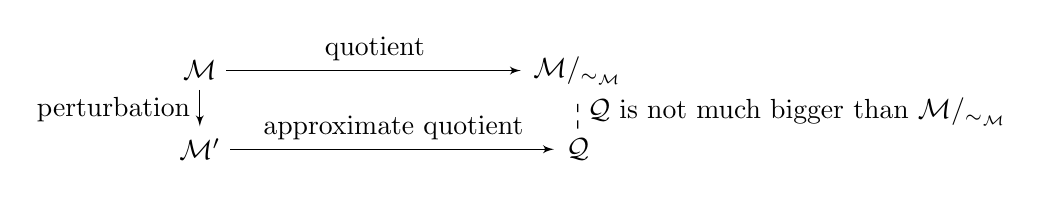
\begin{tikzpicture}[xscale=.6,>=latex',shorten >=1pt,node distance=3cm,on grid,auto]
	
	\node[label] (M) at (0,0) {$\M$};
	\node[label] (MQ) at (8,0) {$\M /_{\sim_{\M}}$};
	\node[label] (Me) at (0,-1) {$\Hyp$};
	\node[label] (MeQ) at (8,-1) {$\Q$};
	
	\path[->] (M) edge node [midway, above] {quotient} (MQ);
	\path[->] (M) edge node [midway, left] {perturbation} (Me);
	\path[->] (Me) edge node [midway, above] {approximate quotient} (MeQ);		
	\path[dashed] (MeQ) edge node [midway, right] {$\Q$ is not much bigger than $\M /_{\sim_{\M}}$} (MQ);		
	%\path[->] (Meq) edge node [midway, below] {minimisation} (MOut);				
	\end{tikzpicture}
	\caption{Problem setup.}\label{fig:problem-setup}
\end{figure}
%NP-hard to obtain minimum approximate quotient

Recall from the introduction that we are given an LMC $\Hyp$, which is a slightly perturbed version of an (unknown) LMC $\M$. By slightly perturbed we mean that for each state the successor distributions in $\Hyp$ and~$\M$ have small (say, less than~$\epsilon$) $L_1$-distance. For example, with sampling we can obtain with high probability a perturbed system that has small distance with $\M$. Assume there are many symmetries, that is, lots of probabilistic bisimilar states in $\M$. The state space of $\M$ can then be compressed a lot by (exact) quotienting. Since the transition probabilities are perturbed in $\Hyp$, the states that are probabilistic bisimilar in $\M$ might become inequivalent in $\Hyp$; as a result, the (exact) bisimulation quotient of $\Hyp$ is much larger than that of $\M$. Given a small compression parameter $\errorParam \gr 0$, we aim to compute an approximate quotient $\Q$, an $\epsilon'$-quotient of $\Hyp$ that satisfies two conditions: \modify{(1) $\epsilon'$ should be small, so that little precision is
sacrificed; and (2) the state space of the quotient should be small, to speed up
verification algorithms. Our contribution consists of approximate quotienting algorithms with (a) theoretical guarantees on goal (1) in \cref{theorem:bounding-global-distance} and
\cref{corollary:bounding-quotient-error}, applying to both algorithms: $\epsilon'$ is bounded (and can be controlled) by a compression parameter $\epsilon_2$ and
the number of iterations $i$; (b) empirical results on goal (2): the experiments show that our algorithms produce small quotients.} %(1) $\epsilon'$ is not much bigger than $\errorParam$; and (2) $\Q$ is not much bigger than $\M/_{\sim_{\M}}$, the quotient of $\M$. \cref{fig:problem-setup} shows the setup of our problem.

We first show that it is hard to find an $\errorParam$-quotient of $\Hyp$ with minimum number of states: $\Q^{*}= \arg\min\{|\Q| : \Q \text{ is an } \errorParam\text{-quotient of }\Hyp\}.$ If there are several $\errorParam$-quotients of $\Hyp$ of minimum size, $\Q^{*}$ can be taken to be any one of them. Unfortunately, this problem is unlikely to have an efficient (polynomial-time) solution, as we will see from the next theorem that the decision version of this problem is $\sf NP$-complete.


\begin{figure}[h]
	\begin{minipage}{0.45\linewidth}
		\centering
		
		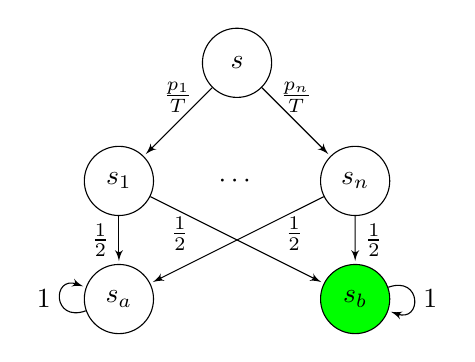
\begin{tikzpicture}[xscale=.6,>=latex',shorten >=1pt,node distance=3cm,on grid,auto]
		
		\node[state] (us) at (3,4) {$s$};
		\node[state] (u1) at (0.5,2.5) {$s_{1}$};
		\node[label] at (3,2.5) {$\cdots$};
		\node[state] (un) at (5.5,2.5) {$s_{n}$};
		
		
		\node[state] (qb) at (0.5,1) {$s_a$};
		\node[state, fill=green] (qc) at (5.5,1) {$s_b$};
		
		\path[->] (us) edge node  [midway,above] {$\frac{p_1}{T}$} (u1);
		\path[->] (us) edge node  [midway,above] {$\frac{p_n}{T}$} (un);
		
		
		\path[->] (qc) edge  [loop right] node [right] {$1$} (qc);
		\path[->] (qb) edge [loop left] node [left]{$1$} (qb);
		
		\path[->] (u1) edge node  [midway,left] {$\frac{1}{2}$} (qb);
		\path[->] (u1) edge node  [very near start, below,xshift=0.1cm] {$\frac{1}{2}$} (qc);
		\path[->] (un) edge node [very near start, below,xshift=-0.1cm] {$\frac{1}{2}$} (qb);
		\path[->] (un) edge node [midway,right] {$\frac{1}{2}$} (qc);
		
		\end{tikzpicture}
		
	\end{minipage}
	\hspace{0.5cm}
	\begin{minipage}{0.45\linewidth}
		\centering
		
		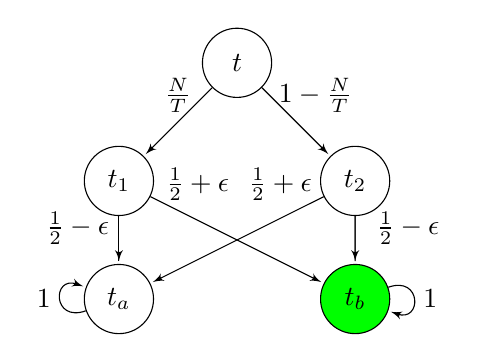
\begin{tikzpicture}[xscale=.6,>=latex',shorten >=1pt,node distance=3cm,on grid,auto]
		
		\node[state] (t) at (2,4) {$t$};
		
		\node[state] (t1) at (-0.5,2.5) {$t_1$};
		\node[state] (t2) at (4.5,2.5) {$t_2$};
		
		\node[state] (qb) at (-0.5,1) {$t_a$};
		\node[state, fill=green] (qc) at (4.5,1) {$t_b$};
		
		\path[->] (t) edge node [midway, above] {$\frac{N}{T}$} (t1);
		\path[->] (t) edge node [midway, above, xshift=0.25cm] {$1-\frac{N}{T}$} (t2);
		
		\path[-] (t1) edge node [midway, right] {} (qb);
		\path[->] (t1) edge node [near start, left] {$\frac{1}{2} - \epsilon$} (qb);
		\path[->] (t1) edge node [near start, above,xshift=0.05cm,yshift=0.1cm] {$\frac{1}{2} + \epsilon$} (qc);
		
		\path[-] (t2) edge node [midway, right] {} (qc);		
		\path[->] (t2) edge node [near start, above, yshift=0.1cm] {$\frac{1}{2}+ \epsilon$} (qb);
		\path[->] (t2) edge node [near start, right,xshift=0.15cm] {$\frac{1}{2} - \epsilon$} (qc);
		
		\path[->] (qc) edge [loop right] node [midway, right] {$1$} (qc);
		\path[->] (qb) edge [loop left]   node [midway, left]{$1$} (qb);
		
		\end{tikzpicture}
	\end{minipage}
	\caption{The LMC in the reduction for {\sf NP}-hardness. All states have the same label $a$ except $s_b$ and $t_b$ which have label $b$.
	}\label{fig:reductionfromSubsset}
\end{figure}

Given an LMC $\Hyp$, a compression parameter $\errorParam \gr 0$ and a constant $k \in \integer^{+}$, it is {\sf NP}-complete to decide whether there exists an $\errorParam$-quotient of $\Hyp$ of size $k$. The hardness result is by reduction from the Subset Sum problem. Given a set $P =\{p_1, \ldots, p_n\}$ and $N \in \nat$, Subset Sum asks whether there exists a set $Q \subseteq P$ such that $\sum_{p_i \in Q} p_i = N$. Given an instance of Subset Sum $<P, N>$ where $P =\{p_1, \ldots, p_n\}$ and $N \in \nat$, we construct an LMC; see \cref{fig:reductionfromSubsset}. Let $T = \sum_{p_i \in P} p_i$, $\epsilon = \frac{1}{2T}$ and $k = 5$. \modify{In the LMC, state $s$ transitions to state $s_i$ with probability $p_i / T$ for all $1 \le  i \le n$. Each state $s_i$ transitions to $s_a$ and $s_b$ with equal probabilities. State $t$ transitions to $t_1$ and $t_2$ with probability $N / T$ and $1 - N / T$, respectively. State $t_1$ (resp. $t_2$) transitions to $t_a$ (resp. $t_b$) and $t_b$ (resp. $t_a$) with probability $\frac{1}{2} - \epsilon$ and $\frac{1}{2} + \epsilon$, respectively. All the remaining states transition to the successor state with probability one. States $s_b$ and $t_b$ have label $b$ and all other states have label $a$.} We can show that $<P, N> \in {\mbox{Subset Sum}} \iff$ there exists an $\frac{1}{2T}$-quotient of $\Hyp$ of size $5$.

\begin{restatable}{theorem}{theoremMinimumApproximateQuotientNPComplete}\label{theorem: minimum-approximate-quotient-NP-complete}
	Given an LMC $\Hyp$, $\errorParam \in (0, 1]$ and $k \in \integer^{+}$. The problem whether there exists an $\errorParam$-quotient of $\Hyp$ of size $k$ is $\sf NP$-complete. It is $\sf NP$-hard even for (fixed) $k=5$.
\end{restatable}

Due to the $\sf NP$-hardness result, we hope to develop practical algorithms to compute approximate quotients of $\Hyp$ that are small but not necessarily of minimum size. To do that, an intuitive idea is to merge ``similar'' states. As we have discussed in the introduction, merging states with small probabilistic bisimilarity distances might be insufficient. Consider the LMC shown in \cref{fig:intro3}. Assume $\epsilon \gr 0$. The states $s_1$ and $t_1$ ($s_2$ and $t_2$) have probabilistic bisimilarity distance one. Thus, to merge $s_1$, $t_1$ or $s_2$, $t_2$, one needs to merge states with probabilistic bisimilarity distance one. Alternatively, we explore the relation of approximate quotient and $\epsilon$-bisimulation. It is not hard to prove the following proposition:%that if $\Q$ is an $\errorParam$-quotient of $\Hyp$, in the LMC $\Hyp \oplus \Q$, for all $s$ from $\Hyp$ we have $s \sim_{\frac{\errorParam}{2}} [s]^{\errorParam}$. %We will see later by examples that the idea of merging states with small approximate probabilistic bisimilar distances does not work.


\begin{restatable}{proposition}{propositionApproximateGlobalRelationSubset}\label{proposition:approximate-quotient-implies-approximate-bisimulation}
	Let $\Q$ be an $\errorParam$-quotient of $\Hyp$. Then in the LMC $\Hyp \oplus \Q$, we have $s \sim_{\frac{\errorParam}{2}} [s]^{\errorParam}_{\Q}$ for all $s$ from $\Hyp$.
\end{restatable}

\begin{figure}[t]
	\centering
	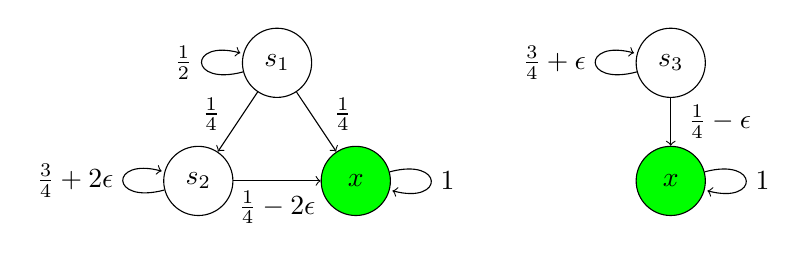
\begin{tikzpicture}
	\tikzstyle{BoxStyle} = [draw, circle, fill=black, scale=0.05,minimum width = 0.001pt, minimum height = 0.001pt]
	\node[state] (s) at (3,4) {$s_1$};
	\node[state] (s1) at (2,2.5) {$s_{2}$};
	\node[state, fill=green] (x) at (4,2.5) {$x$};
	\path[->] (s) edge [loop left] node  [midway,left] {$\frac{1}{2}$} (s);
	\path[->] (s) edge node  [midway,left,xshift=-0.1cm,yshift=0.1cm] {$\frac{1}{4}$} (s1);
	\path[->] (s) edge node  [midway,right,xshift=0.1cm,yshift=0.1cm] {$\frac{1}{4}$} (x);
	\path[->] (x) edge [loop right] node [midway, right] {$1$} (x);
	\path[->] (s1) edge node  [midway,below] {$\frac{1}{4}-2\epsilon$} (x);
	\path[->] (s1) edge [loop left] node [midway, left] {$\frac{3}{4} + 2\epsilon$} (s1);
	
	\node[state] (t) at (8,4) {$s_3$};
	\node[state, fill=green] (y) at (8,2.5) {$x$};
	\path[->] (t) edge [loop left] node  [midway,left] {$\frac{3}{4}+\epsilon$} (t);
	\path[->] (t) edge node  [midway,right,xshift=0.1cm] {$\frac{1}{4}-\epsilon$} (y);
	\path[->] (y) edge [loop right] node [midway, right] {$1$} (y);
	
	%	\node[state] (ss1) at (7,4) {$s_1$};
	%	\node[state, fill=green] (z) at (7,2.5) {$x$};
	%	\path[->] (ss1) edge [loop left] node  [midway,left] {$\frac{3}{4}+2\epsilon$} (ss1);
	%	\path[->] (ss1) edge node  [midway,right,xshift=0.1cm] {$\frac{1}{4}-2\epsilon$} (z);
	%	\path[->] (z) edge [loop right] node [midway, right] {$1$} (z);
	\end{tikzpicture}
	\caption{An LMC in which $s_1 \sim_{\epsilon} s_3 \sim_{\epsilon} s_2$.}
	\label{fig:exampleGlobal}
\end{figure}
\begin{figure}[t]
	\centering
	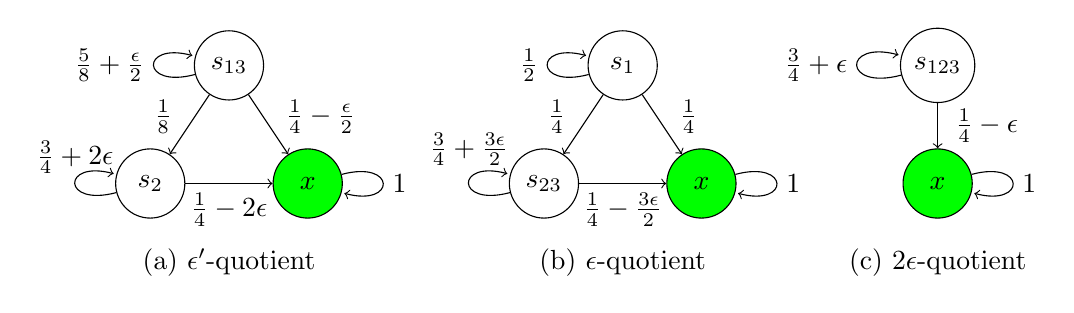
\begin{tikzpicture}
	\tikzstyle{BoxStyle} = [draw, circle, fill=black, scale=0.05,minimum width = 0.001pt, minimum height = 0.001pt]
	\node[state] (s) at (3,4) {$s_{13}$};
	\node[state] (s1) at (2,2.5) {$s_{2}$};
	\node[state, fill=green] (x) at (4,2.5) {$x$};
	\path[->] (s) edge [loop left] node  [midway,left] {$\frac{5}{8}+\frac{\epsilon}{2}$} (s);
	\path[->] (s) edge node  [midway,left,xshift=-0.1cm,yshift=0.1cm] {$\frac{1}{8}$} (s1);
	\path[->] (s) edge node  [midway,right,xshift=0.1cm,yshift=0.1cm] {$\frac{1}{4}-\frac{\epsilon}{2}$} (x);
	\path[->] (x) edge [loop right] node [midway, right] {$1$} (x);
	\path[->] (s1) edge node  [midway,below] {$\frac{1}{4}-2\epsilon$} (x);
	\path[->] (s1) edge [loop left] node [midway, above] {$\frac{3}{4} + 2\epsilon$} (s1);
	\node at (3, 1.5) {(a) $\epsilon'$-quotient};
	
	\node[state] (s) at (8,4) {$s_1$};
	\node[state] (s1) at (7,2.5) {$s_{23}$};
	\node[state, fill=green] (x) at (9,2.5) {$x$};
	\path[->] (s) edge [loop left] node  [midway,left] {$\frac{1}{2}$} (s);
	\path[->] (s) edge node  [midway,left,xshift=-0.1cm,yshift=0.1cm] {$\frac{1}{4}$} (s1);
	\path[->] (s) edge node  [midway,right,xshift=0.1cm,yshift=0.1cm] {$\frac{1}{4}$} (x);
	\path[->] (x) edge [loop right] node [midway, right] {$1$} (x);
	\path[->] (s1) edge node  [midway,below] {$\frac{1}{4}-\frac{3\epsilon}{2}$} (x);
	\path[->] (s1) edge [loop left] node [midway, above,yshift=0.1cm] {$\frac{3}{4} + \frac{3\epsilon}{2}$} (s1);	
	\node at (8, 1.5) {(b) $\epsilon$-quotient};
	
	\node[state] (t) at (12,4) {$s_{123}$};
	\node[state, fill=green] (y) at (12,2.5) {$x$};
	\path[->] (t) edge [loop left] node  [midway,left] {$\frac{3}{4}+\epsilon$} (t);
	\path[->] (t) edge node  [midway,right,xshift=0.1cm] {$\frac{1}{4}-\epsilon$} (y);
	\path[->] (y) edge [loop right] node [midway, right] {$1$} (y);
	\node at (12, 1.5) {(c) $2\epsilon$-quotient};	
	%	\node[state] (ss1) at (7,4) {$s_1$};
	%	\node[state, fill=green] (z) at (7,2.5) {$x$};
	%	\path[->] (ss1) edge [loop left] node  [midway,left] {$\frac{3}{4}+2\epsilon$} (ss1);
	%	\path[->] (ss1) edge node  [midway,right,xshift=0.1cm] {$\frac{1}{4}-2\epsilon$} (z);
	%	\path[->] (z) edge [loop right] node [midway, right] {$1$} (z);
	\end{tikzpicture}
	\caption{(a) An $\epsilon'$-quotient obtained by merging $s_1$ and $s_3$ where $\epsilon'$ is at least $\frac{1}{4}+\epsilon$; (b) An $\epsilon$-quotient obtained by merging $s_2$ and $s_3$; (b) A $2\epsilon$-quotient obtained by merging $s_1$, $s_2$ and $s_3$.}
	\label{fig:exampleMerge}
\end{figure}

\cref{proposition:approximate-quotient-implies-approximate-bisimulation} suggests that $\epsilon_2$-quotients and $\epsilon_2$-bisimulation are related.  The runtime of the algorithm to compute the $\epsilon_2$-bisimulation in \cite{DesharnaisLavoletteTracol2008} is $O(|S|^7)$ which makes it not practical for large systems. Furthermore, the algorithms based on merging states that are $\epsilon_2$-bisimilar may produce an $\epsilon'$-quotient where $\epsilon'$ is large, violating the first condition of a satisfying approximate quotient. Assume the positive number $\epsilon$ is much smaller than $\frac{1}{8}$. Let us choose the compression parameter $\epsilon_2$ to be the same as $\epsilon$. We compute the $\epsilon$-bisimulation of the LMC shown in \cref{fig:exampleGlobal} and get $s_1 \sim_{\epsilon} s_3 \sim_{\epsilon} s_2$.  Since $\epsilon$-bisimulation is not an equivalence relation, $s_1  \sim_{\epsilon} s_2$ does not necessarily follow. Indeed, in this LMC, we have $s_1  \sim_{2\epsilon} s_2$ but not $s_1  \sim_{\epsilon} s_2$. If $s_2$ and $s_3$, related by $\sim_{\epsilon}$, are chosen to be merged, the resulting LMC in \cref{fig:exampleMerge}(b) is an $\epsilon$-quotient. However, if $s_1$ and $s_3$ are (unfortunately) chosen to be merged, the resulting LMC, shown in \cref{fig:exampleMerge}(a), is an $\epsilon'$-quotient where $\epsilon'$ cannot be smaller than $\frac{1}{4}+\epsilon$. This $\epsilon'$, much bigger than $\epsilon$ under the assumption that $\epsilon$ is much smaller than $\frac{1}{8}$, makes the resulting LMC undesirable. This example shows that arbitrarily merging states that are $\epsilon$-bisimilar may not work. The LMC in \cref{fig:exampleMerge}(c) is obtained by merging $s_1$, $s_2$ and $s_3$, the states that are related by the transitive closure of $\sim_{\epsilon}$. We show in the appendix that for any $n \in \integer^{+}$ there exists an LMC $\M(n)$ such that merging all states in $\M(n)$  that are related by the transitive closure of $\sim_{\epsilon}$ results in an $\epsilon'$-quotient where $\epsilon'$ is at least $n\epsilon$.

%Since $s R_{\epsilon'} s_1$ does not hold for $\epsilon' \ls 2\epsilon$, we have $s R_{\epsilon'} t$ does not hold for $\epsilon' \ls 2\epsilon$, that is, $s \mathord{R_{\epsilon}} t$ does not hold. This implies that $\mathord{\sim_{\epsilon}} \not\subseteq \mathord{R_{\epsilon}}$. %Together with the previous proposition, we have $R_{\epsilon} \subset \sim_{\epsilon}$.



\cref{lemma:additivity-property}, the additivity lemma, asserts an additivity property of approximate quotients. In \cref{section:minimisation-algorithms}, this lemma will be applied as the two minimisation algorithms successively compute a sequence of approximate quotients.



%TODO parameter continuous

\begin{restatable}{lemma}{lemmaAdditivityProperty}\label{lemma:additivity-property}
		Consider three LMCs $\M_1$, $\M_2$ and $\M_3$. Let $\epsilon_1 \ge 0$ and $\M_2$ be an $\epsilon_1$-quotient of $\M_1$. Let $\epsilon_2 \ge 0$ and $\M_3$ be an $\epsilon_2$-quotient of $\M_2$. Then $\M_3$ is an $(\epsilon_1+\epsilon_2)$-quotient of $\M_1$. %= <S_i, L, \tau_i, \ell_i>$ where $i \in \{1,2,3\}$ and the $S_i$ are pairwise disjoint sets.
\end{restatable}



\section{Approximate Minimisation Algorithms}\label{section:minimisation-algorithms}

\begin{figure}[h]
	\centering
	
	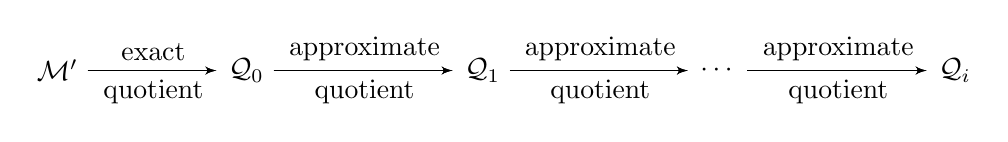
\begin{tikzpicture}[xscale=.6,>=latex',shorten >=1pt,node distance=3cm,on grid,auto]
	
	\node[label] (Me) at (0,0) {$\Hyp$};
	\node[label] (Q0) at (4,0) {$\Q_{0}$};
	\node[label] (Q1) at (9,0) {$\Q_{1}$};
	\node[label] (Qd) at (14,0) {$\cdots$};
	\node[label] (Qi) at (19,0) {$\Q_{i}$};
	
	\path[->] (Me) edge node [midway, above] {exact} (Q0);
	\path[->] (Me) edge node [midway, below] {quotient} (Q0);	
	\path[->] (Q0) edge node [midway, above] {approximate} (Q1);
	\path[->] (Q0) edge node [midway, below] {quotient} (Q1);	
	\path[->] (Q1) edge node [midway, above] {approximate} (Qd);	
	\path[->] (Q1) edge node [midway, below] {quotient} (Qd);				
	\path[->] (Qd) edge node [midway, above] {approximate} (Qi);		
	\path[->] (Qd) edge node [midway, below] {quotient} (Qi);		
	%\path[->] (Meq) edge node [midway, below] {minimisation} (MOut);				
	\end{tikzpicture}
	\caption{Overview of the minimisation algorithms. \cref{lemma:additivity-property} applies to $\Hyp$, $\Q_{0}$, $\Q_{1}, \cdots, \Q_{i}$.}\label{fig:algorithms}
\end{figure}

In this section, we present two practical minimisation algorithms that compute approximate quotients of $\Hyp$. Given an LMC $\Hyp = <S, L, \tauHyp, \ell>$ with perturbed transition probabilities and a small compression parameter $\epsilon_2$. Both algorithms start by computing $\Q_0$, the exact quotient of $\Hyp$.  They proceed in iterations and compute a sequence of approximate quotients where the approximate quotient ($\Q_{i}$) computed at the end of the $i$th iteration is an $\epsilon_2$-quotient of the quotient ($\Q_{i-1}$) given at the beginning of that iteration. Using the additivity lemma, we can show that the (approximate) quotient $\Q_i$ after the $i$th iteration is an $i\epsilon_2$-quotient of $\Hyp$. See \cref{fig:algorithms} for an overview of this approach. Each iteration computes a partition of the state space, lumps the states that are together in the partition and concludes with taking the exact quotient.

%In this section, we present two practical minimisation algorithms that compute approximate quotients of $\Hyp$. Both algorithms proceed in iterations and compute a sequence of approximate quotients. In each iteration, the algorithms first compute a partition of the state space of an approximate quotient and then lump the states that are together in the partition. The exact quotient of the LMC after lumping is used as the new approximate quotient. The first approximate quotient $\Q_0$ is obtained by (exact) quotienting $\Hyp$ and it is guaranteed that the new approximate quotient obtained after lumping is an $\epsilon_2$-approximate quotient of the LMC before lumping. Using the additivity lemma, we can show that the approximate quotient generated by either algorithm after the $i$'s iteration is an $i\epsilon_2$-quotient of $\Hyp$. See \cref{fig:algorithms} for an overview of the algorithms.

\subsection{Local Bisimilarity Distance}\label{subsection:local-bisimilarity-distances}

We define the notion of \emph{local bisimilarity distance}, denoted by $d_{\local}^{\M}$ (or $d_{\local}$ when $\M$ is clear). Intuitively, two states $s$ and $t$ are at small local bisimilarity distance if they are probabilistic bisimilar in an LMC which is slightly perturbed only at the successor distributions of $s$ and~$t$. We provide a polynomial-time algorithm to compute the local bisimilarity distance. Given an LMC $\Hyp = <S, L, \tauHyp, \ell>$ (with perturbed transition probabilities) and a small compression parameter $\epsilon_2$, we propose an iterative minimisation algorithm to compute approximate quotients of $\Hyp$ by merging state pairs with small local bisimilarity distances. In each iteration of the algorithm, we select the state pair with the same label and the minimum local bisimilarity distance if such distance is at most $\epsilon_2$. We compute a partition in which this state pair are together and lump together the states that are together in the partition. The algorithm terminates when no pairs can be lumped, that is, all state pairs have local bisimilarity distances greater than $\epsilon_2$. %The LMC after lumping a state pair is an $\epsilon_2$-approximate quotient of the LMC before merging. Using the additivity lemma, the approximate quotient obtained by this algorithm after the $i$'s iteration is an $i\epsilon_2$-quotient of $\Hyp$.

% We then merge the states for which this distance is small. For the remainder of the section, we fix an approximation LMC $\Hyp = <S, L, \tauHyp, \ell>$ and a small error parameter $\epsilon_2$. The minimisation algorithm runs in iterations. In each iteration, we compute the local bisimilarity distances for all pairs of states with the same label. We merge the pair of states $s$ and $t$ with the same label such that it has the minimum local bisimilarity distance at most $\epsilon_2$. The algorithm terminates when no pairs can be merged, that is, all pairs of states have local bisimilarity distance greater than $\epsilon_2$.

 \paragraph*{Computing Local Bisimilarity Distances}\label{subsubsection:computeLocalBisimilarityDistances}
Given two different states $s, t \in S$ with the same label. We want to compute a new transition function $\tauHyp'$ by only changing the successor distributions of $s$ and $t$ ($\tauHyp(s)$ and $\tauHyp(t)$, respectively) such that $\{s, t\}$ belongs to an $\R$-induced partition where $\R$ is a probabilistic bisimulation of the LMC $\Hyp' = <S, L, \tauHyp', \ell>$. Let ${\rm T}$ be the set of the all transition functions that satisfy this condition, more precisely, we define ${\rm T} = \{\tauHyp' \suchthat \tauHyp'(x) = \tauHyp(x) \; \forall x \not\in \{s, t\}  \land \{s, t\} \in S /_{\R} \text{ where } \R \text{ is a probabilistic bisimulation of the LMC } \Hyp' = <S, L, \tauHyp', \ell>\}$. The local bisimilarity distance is defined as $d_{\local}^{\Hyp}(s, t) = \textstyle\inf_{\tau' \in {\rm T}} \max\{\|\tau'(s) - \tauHyp(s)\|_1, \|\tau'(t) - \tauHyp(t)\|_1 \}$. It is not immediately clear how to compute it. %Since for all $\tau' \in {\rm T}$, we have $s \sim t$ in the LMC $<S, T, \tau', \ell>$, it is not hard to see that $d^{\Hyp}_{\glob}(s, t) \le d_{\local}^{\Hyp}(s, t)$, that is, $d_{\local}^{\Hyp}(s, t)$ is an upper bound of $d^{\Hyp}_{\glob}(s, t)$.

%[not working] the required partition can be obtained simply by the following three steps: (1) construct a new LMS M’ from M by making both s and t absorbing; (2) compute the equivalence classes Y of M’ according to probabilistic bisimilarity; (3) delete s and t from Y and put back a new equivalence class {s, t}.
By the definition of ${\rm T}$, the probabilistic bisimulation $\R$ is the same for any LMC $<S, L, \tauHyp', \ell>$ with $\tauHyp' \in {\rm T}$. Let us define the partition $X = S /_\R$ where $\R$ is the common probabilistic bisimulation. The local bisimilarity distance can be computed by using $X$:
%Let us fix a transition function $\tauHyp' \in {\rm T}$ and fix an LMC $\Hyp' = <S, L, \tauHyp', \ell>$. To compute the local bisimilarity distance, we first compute the partition $X$ containing $\{s, t\}$ which is induced by the probabilistic bisimulation $\R$ of the LMC $\Hyp'$. It is noted that by the definition of ${\rm T}$, the probabilistic bisimulation $\R$ is the same for any LMC $<S, L, \tau', \ell>$ with $\tau' \in {\rm T}$. We then show that the local bisimilarity distance is half of the $L_1$-distance between $(\tau_{\epsilon}(s)(E))_{E \in X}$ and $(\tau_{\epsilon}(t)(E))_{E \in X}$: %, that is, $d_{\local}^{\Hyp}(s, t) = \frac{1}{2} |(\tau_{\epsilon}(s)(E))_{E \in X} -(\tau_{\epsilon}(s)(E))_{E \in X}|$.

%The partition $X = S /_{\R}$ can simply be computed by the following two steps: (1) construct a new LMC from $\Hyp$ by introducing a new label, labelling both $s$ and $t$ with the new label and making both $s$ and $t$ absorbing; (2) compute the equivalence classes of this new LMC according to probabilistic bisimilarity. The resulting equivalence classes is $X$.  %by \cref{alg:s-t-partition-refinement}. Given a partition $Y$, we say $u \equiv_{Y} v$ in the LMC $<S, L, \tauHyp, \ell>$ if and only if $\ell(u) = \ell(v)$ and $\tauHyp(u)(E) = \tauHyp(v)(E)$ for all $E \in Y$.


%By definition of the set $\rm T$, the probabilistic bisimulation which contains $\{s, t\}$ of an LMC $\Hyp' = <S, L, \tauHyp', \ell>$ is the same for any $\tauHyp' \in {\rm T}$. This common probabilistic bisimulation induces a common partition over $S$, denoted by $X$, which is computed by \cref{alg:s-t-partition-refinement}.



%\begin{algorithm}[h]
%	\DontPrintSemicolon
%	
%	$i = 0; Y_0 := \big\{ \{s, t\}, S \setminus \{s, t\} \big\}$\;
%	\Repeat{$Y_i = Y_{i-1}$}{
%		$i := i+1$\;
%		$Y_{i} :=S/\mathord{\equiv_{Y_{i-1}}}$ \;
%		$Y_{i} := \big( (Y_{i} \setminus \{s\} ) \setminus \{t\} \big)  \cup \{\{s, t\}\}$\;
%	}
%	\caption{Partition refinement with $\{s, t\}$ in the final partition.}
%	\label{alg:s-t-partition-refinement}
%\end{algorithm}


\begin{restatable}{proposition}{propositionAdjustTransitionFunction}\label{proposition:adjust-transition-function-s-t}
%We have $d_{\local}^{\Hyp}(s, t) = \max\{|\tauHyp'(s) - \tauHyp(s)|, |\tauHyp'(t) - \tauHyp(t)| \} $ where $\tauHyp' \in {\rm T}$ is defined as \[
%\tauHyp'(x) = \left \{
%\begin{array}{ll}
%\tauHyp(x)& \mbox{if $x \not\in \{s, t\}$}\\
%\nu_x & \mbox{otherwise}
%\end{array}
%\right .
%\]
%Furthermore,
We have $d_{\local}^{\Hyp}(s, t) =	 \frac{1}{2} \|(\tau_{\epsilon}(s)(E))_{E \in X} -(\tau_{\epsilon}(t)(E))_{E \in X}\|_1$.
%We have $d_{\local}^{\Hyp}(s, t) = \max\{ |\tauHyp'(s) - \tauHyp(s)| , |\tauHyp'(t) - \tauHyp(t)|\}$ where
%$\tauHyp' \in {\rm T}$ is defined as $\tauHyp'(x) = \tauHyp(x)$ for all $x \not\in \{s, t\}$ and $\tauHyp'(x) = \nu_x$ if $x \in \{s, t\}$.
\end{restatable}

It turns out that $X$ can simply be computed by \cref{alg:local-distance-partition}. As this algorithm is basically taking the (exact) quotient of the LMC constructed on line~1, it runs in polynomial time. It follows from \cref{proposition:adjust-transition-function-s-t} that the local bisimilarity distance can be computed in polynomial time.

%The partition $X = S /_{\R}$ can simply be computed by the following two steps: (1) construct a new LMC from $\Hyp$ by introducing a new label, labelling both $s$ and $t$ with the new label and making both $s$ and $t$ absorbing; (2) compute the equivalence classes of this new LMC according to probabilistic bisimilarity. The resulting equivalence classes constitute $X$.  %by \cref{alg:s-t-partition-refinement}. Given a partition $Y$, we say $u \equiv_{Y} v$ in the LMC $<S, L, \tauHyp, \ell>$ if and only if $\ell(u) = \ell(v)$ and $\tauHyp(u)(E) = \tauHyp(v)(E)$ for all $E \in Y$.

\begin{algorithm}[h]
	\DontPrintSemicolon
	\KwIn{An LMC $\Hyp = <S, L, \tauHyp, \ell>$, a state pair $(s, t) \in S \times S$}
	\KwOut{A partition $X$ over $S$ containing $\{s, t\}$}
	Construct a new LMC $\Hyp'$ from $\Hyp$ by introducing a new label, labelling both $s$ and $t$ with the new label and making both $s$ and $t$ absorbing\footnotemark\;
	$X := S /_{\sim_{\Hyp'}}$\;
	\caption{Compute Partition for Local Bisimilarity Distances}
	\label{alg:local-distance-partition}
\end{algorithm}
\footnotetext{\modify{An absorbing state is a state that, once entered, cannot be left; that is, a state with self-loop.}}

\begin{example}\label{example:intro3}
 Assume $\epsilon \ls \frac{1}{2}$. Consider the LMC shown in \cref{fig:intro3}. Let $\tauHyp$ denote its transition function. To compute the local bisimilarity distance of $s_1$ and $t_1$, we first compute the partition containing $\{s_1, t_1\}$: $X = \big\{ \{ s_1, t_1\}, \{ s_2\},\{ t_2\} \big\}$. We have $(\tauHyp(s_1)(E))_{E \in X} = (\frac{1}{2}, \frac{1}{2}, 0)$ and $(\tauHyp(t_1)(E))_{E \in X} = (\frac{1}{2}+\epsilon, 0, \frac{1}{2}-\epsilon)$. By \cref{proposition:adjust-transition-function-s-t}, the local bisimilarity distance is $d_{\local}(s_1, t_1) = \frac{1}{2}\|(\tauHyp(s_1)(E))_{E \in X} -(\tauHyp(t_1)(E))_{E \in X}\|_1 = \frac{1}{2}$. Similarly, we have~$d_{\local}(s_2, t_2) =~\frac{1}{2}$.%~\qed
\end{example}

\begin{algorithm}[h]
	\DontPrintSemicolon
	\KwIn{An LMC $\Hyp = <S, L, \tauHyp, \ell>$, a compression parameter $\epsilon_2$}
	\KwOut{An LMC $\Q_{i}$}
	$i := 0$\\
	%$\M^{i}: = <S, L, \tau', \ell>$ \\	
	%Compute $\sim_{\Hyp}$\\
	$\Q_{i} := \Hyp/_{\sim_{\Hyp}}$ and $\Q_{i} = <S^{\Q_{i}}, L, \tau^{\Q_{i}}, \ell^{\Q_{i}}>$\;
	%$\Q_{i} = <S^{\Q_{i}}, L, \tau^{\Q_{i}}, \ell^{\Q_{i}}> := \M^{i}/_{\sim_{\M^{i}}}$ where $\M^{i} = \Hyp$\\	
	%$\Hyp^{i} = <S^{\Hyp^{i}}, L, \tau^{\Hyp^{i}}, \ell^{\Hyp^{i}}> := \M^{i}/_{\sim_{\M^{i}}}$ where $\M^{i} = \Hyp$\\
	\While{$\exists u, v \in S^{\Q_{i}} \text{ such that }  u \not= v \text{ and }  \ell^{\Q_{i}}(u) = \ell^{\Q_{i}}(v) \text{ and }  d_{\local}^{\Q_{i}} (u, v) \le \epsilon_2$ }{
		$(s, t) = \arg\min \{d_{\local}^{\Q_{i}} (u, v) \suchthat (u ,v) \in S^{\Q_{i}} \times S^{\Q_{i}} \land u \not= v \land   \ell^{\Q_{i}}(u) = \ell^{\Q_{i}}(v)\}$\\
		%Select two states $s, t \in S^{\Hyp^{i}}$ where $\ell^{\Hyp^{i}}(s) = \ell^{\Hyp^{i}}(t)$ and $d_{\local}^{\Hyp^{i}} (s, t) = \min\limits_{u ,v \in S^{\Hyp^{i}} \text{ and } \ell^{\Hyp^{i}}(u) = \ell^{\Hyp^{i}}(v)} d_{\local}^{\Hyp^{i}} (u, v)$\\
		%Compute $\sim_{\Hyp^{i}}$\\
		%		Compute $X$ by Algorithm~\ref{alg:s-t-partition-refinement} with the input LMC $\Hyp^{i}$ and $\{s, t\}$\;
		%		$\gamma := \frac{(\tau^{\Hyp^{i}}(s))_{E \in X} + (\tau^{\Hyp^{i}}(t))_{E \in X}}{2}$ \;
		%		$\nu_s$ (resp. $\nu_t$) is obtained by running \cref{alg:adjust-transition-probability} with $X$, $\tau^{\Hyp^{i}}(s)$ (resp. $\tau^{\Hyp^{i}}(t)$) and $\gamma$\;
		%		$
		%		\tau'(x) := \left \{
		%		\begin{array}{ll}
		%		\tau^{\Hyp^{i}}(x)& \mbox{if $x \not\in \{s, t\}$}\\
		%		\nu_x & \mbox{otherwise}
		%		\end{array}
		%		\right .
		%		$\;
		%		$\M^{i+1} := <S^{\Hyp^{i}}, L, \tau', \ell^{\Hyp^{i}}>$ \;
		%Construct an LMC $\Q_{i}'$ from $\Q_{i}$ by adding a new label, labelling $s$ and $t$ with this new label and making $s$ and $t$ absorbing \; %$\M_{i+1}$
		%Compute $\M_{i+1}: = \Q_{i}'/_{\sim_{\Q_{i}'}}$ with state space $X_i := S^{\Q_{i}'} /_{\sim_{\Q_{i}'}}$\;
		Compute $X_i$ by running \cref{alg:local-distance-partition} with input $Q_i$ and $(s, t)$\;
		Construct an LMC $\M_{i+1}:= <X_i, L, \tau^{\M_{i+1}}, \ell^{\M_{i+1}}>$ from $\Q_{i}$ where
		$
		\tau^{\M_{i+1}}(E) := \left \{
		\begin{array}{l}
		 (\tau^{\Q_{i}}(u)(E'))_{E' \in X_i}  \mbox{ for any $u \in E$ if $E \in X_i$  and $E \not= \{s, t\}$}\\
		\frac{(\tau^{\Q_{i}}(s)(E'))_{E' \in X_i} + (\tau^{\Q_{i}}(t)(E'))_{E' \in X_i}}{2} \;\; \mbox{if $E = \{s, t\}$}\\
		\end{array}
		\right .
		$ and $\ell^{\M_{i+1}} (E) := \ell^{\Q_i}(u)$ for $E \in X_i$ and any $u \in E$\;
		
		%from $\Q_{i}$ by restoring the labels of $\{s, t\}$ and setting the probability distribution from $\{s, t\}$ as $\frac{(\tau^{\Q_{i}}(s))_{E \in X_i} + (\tau^{\Q_{i}}(t))_{E \in X_i}}{2}$\;
		%Obtain the new approximate quotient LMC $\Q_{i+1}$ by quotienting $\M_{i+1}'$, that is,
		$\Q_{i+1} := \M_{i+1} /_{\sim_{\M_{i+1}}}$\;
		$i := i+1$\;
	}
	\caption{LMC Minimisation Using Local Bisimilarity Distances}
	\label{alg:local-distance-merge-algorithm}
\end{algorithm}

\paragraph*{Minimisation Algorithm Using Local Bisimilarity Distances}
\label{subsubsection:minimisation-algorithm-local-bisimilarity-distances}
\cref{alg:local-distance-merge-algorithm} shows the minimisation algorithm using local bisimilarity distances. The input is an LMC $\Hyp$ and a compression parameter $\epsilon_2$. We start by initializing an index $i$ to $0$ and building the quotient LMC $\Q_{0} = \Hyp /_{\sim_{\Hyp}}$. If there are no states in $\Q_{i}$ with local bisimilarity distance less than $\epsilon_2$, the algorithm terminates. Otherwise, it steps into the $i$'th iteration of the loop and computes the local bisimilarity distances for all pairs of states in $\Q_{i}$ with the same label. It selects the state pair $(s, t)$ which has the smallest local bisimilarity distance on line~4. It then computes the new approximate quotient by merging states $s$ and $t$ on line~$5$-$7$. This computation is in three steps where the first step is to compute the partition $X_i$ (line~5) by running \cref{alg:local-distance-partition} with input $\Q_i$ and the state pair $(s, t)$. The second step is to construct a new LMC $\M_{i+1}$ by setting $X_i$ as its state space (line~6). The final step is to compute a new approximate quotient $\Q_{i+1}$ by taking the exact quotient of the LMC $\M_{i+1}$ obtained from the previous step.
%A new transition function $\tau'$ (line~5-8) as described by \cref{proposition:adjust-transition-function-s-t} and a new LMC $\M^{i+1}$ with $\tau'$ as its transition function is constructed on line~9. We then compute its quotient $\Hyp^{i+1} = \M^{i+1} /_{\sim_{\M^{i+1}}}$. The size of the state space of $\Hyp^{i+1}$ will decrease by at least one as $s \sim_{\M^{i+1}} t$.
We increment $i$ at the end of the iteration and continue with another iteration if there are states in $\Q_{i+1}$ with local bisimilarity distance at most $\epsilon_2$. Since there are finitely many states and it is polynomial time to compute the local bisimilarity distances, the algorithm always terminates and runs in polynomial time.
%The first minimisation algorithm is shown in Algorithm~\ref{alg:local-distance-merge-algorithm} . The input is a hypothesis LMC $\Hyp$ and an error parameter $\epsilon_2$. We start by building the quotient LMC $\Hyp^{i} = \Hyp /_{\sim_{\Hyp}}$ with $i$ initialized to $0$. It then steps into a loop with incrementing $i$ at the beginning. In the $i$'th iteration of the loop, it computes the local bisimilarity distances for all pairs of states in $\Hyp^{i-1}$ with the same label and selects the pair $s$ and $t$ which have the least local bisimilarity distance. We obtain a new LMC $\M^{i}$ by adjusting the transition probability distribution at $s$ and $t$. It is done by replacing the transition function $\tau^{\Hyp^{i-1}}$ of $\Hyp^{i-1}$ with $\tau'' = \adjust(\tau^{\Hyp^{i-1}}, s, t, u)$ where $\tau''$ yields the local bisimilarity distance of $s$ and $t$, that is, $d_{\local}^{\Hyp^{i-1}} (s, t) = \max\{|\tau^{\Hyp^{i-1}}(s) - \tau''(s) |, |\tau^{\Hyp^{i-1}}(t) - \tau''(t)|\}$. We then build the new quotient LMC $\Hyp^{i} = \M^{i} /_{\sim_{\M^{i}}}$. If the size of the state space of $\Hyp^{i}$ decreases we continue the iteration. Otherwise, the algorithm terminates since there are no states in $\Hyp^{i}$ with local bisimilarity distance less than $\epsilon_2$. Since there are finitely many states, the algorithm always terminates.

%%$\Pr(d_{\glob}^{\M \oplus \Hyp^{i}} (x, x') \le \epsilon + i \epsilon_2) \ge (1-\delta)^{|S|}$
%\begin{restatable}{theorem}{theoremBoundingGlobalDistance}\label{theorem:bounding-global-distance} Let $d_{\glob}^{\M \oplus \Hyp} (x, x') \le \epsilon$ for all state $x$ in $\M$ and the corresponding state $x'$ in $\Hyp$. For all $i \in \nat$, we have $d_{\glob}^{\M \oplus \Hyp^{i}} (x, x') \le \epsilon + i \epsilon_2$ where $x$ is a state in $\M$ and $x'$ is the corresponding state in $\Hyp^{i}$.
%\end{restatable}
%
%
%\begin{corollary}\label{corollary:bounding-global-distance-local-distance}
%	For all $i \in \nat$, we have $\Pr(d_{\glob}^{\M \oplus \Hyp^{i}} (x, x') \le \epsilon + i \epsilon_2) \ge (1-\delta)^{|S|}$ where $x$ is a state in $\M$ and $x'$ is the corresponding state in $\Hyp^{i}$.
%\end{corollary}
%\begin{proof}
%Let $i \in \nat$. Let $x$ be a state from $\M$ and $x'$ be the corresponding state from $\Hyp^{i}$. Let $x_h$ of $\Hyp$ correspond to $x$ of $\M$. By $\Pr(d_{\glob}^{\M \oplus \Hyp} (x, x_h) \le \epsilon ) \ge (1-\delta)^{|S|}$ and \cref{theorem:bounding-global-distance}, we have $\Pr(d_{\glob}^{\M \oplus \Hyp^{i}} (x, x') \le \epsilon + i \epsilon_2) \ge (1-\delta)^{|S|}$.
%\end{proof}

%Merging by approximate partition refinement
\subsection{Minimisation by Approximate Partition Refinement}\label{subsection:approximate-partition-refinement}
%an example LMC that could not be merged by the previous algorithm
Consider the LMC in \cref{fig:intro3}. Assume $\epsilon \ls \frac{1}{2}$ and $\epsilon_2 \ls \frac{1}{2}$. The minimisation algorithm using local bisimilarity distance (Algorithm~\ref{alg:local-distance-merge-algorithm}) cannot merge states $s_1, t_1$ (or $s_2, t_2$) as $d_{\local}(s_1, t_1) = d_{\local}(s_2, t_2)  =\frac{1}{2} \gr \epsilon_2$ as shown by \cref{example:intro3}.

We introduce an approximate partition refinement, a polynomial algorithm similar to the exact partition refinement, which can fix this problem. In the exact partition refinement algorithm, the states will only remain in the same set in an iteration if they have the same label and their probability distributions over the previous partition are the same. Similarly, we design the approximate partition refinement such that states only remain in the same set in an iteration if they have the same label and the $L_1$-distance between the probability distributions over the previous partition is small, say, at most $\epsilon_2$. Given an LMC $\Hyp = <S, L, \tauHyp, \ell>$ with perturbed transition probabilities, the minimisation algorithm using the approximate partition refinement also proceeds in iterations. In each iteration, the approximate partition refinement computes a partition $X$ and then the states which are together in $X$ are  lumped to form a new LMC. To make sure the new LMC is a quotient, we take the (exact) quotient of this LMC as our new approximate quotient. The algorithm continues when there are states that could be lumped, and it terminates when all sets in the partition computed by the approximate partition refinement are singletons, that is, no states can be lumped. %We prove that the LMC after merging is an $\epsilon_2$-approximate quotient of the LMC before merging. Similar to the previous minimisation algorithm, using the additivity lemma, the approximate quotient obtained by this algorithm after the $i$'s iteration is an $i\epsilon_2$-quotient of $\Hyp$.%Using the additivity lemma, we can then bound the error of the final approximate quotient obtained by this algorithm.% guarantees that states in an equivalence class of the final partition have small global bisimilarity distances and thus can be merged.

\modify{
	\begin{example}\label{example:approximate-partition-intro}	
	Consider again the LMC in \cref{fig:intro3}. Assume $\epsilon \ls \frac{1}{2}$ and the compression parameter $\epsilon_2 \ge 2\epsilon$.  We run the above-mentioned minimisation algorithm using the approximate partition refinement. It will only run for one iteration of approximate partition refinement, as we will see in the following. \Cref{fig:example-intro-approximate-partition-refinement}(a) shows the partitions of this iteration. At the beginning of the approximate partition refinement, we have partition $X_0$ as all states are in the same set. The states are then split by the labels and we get partition $X_1$. There is no further split since the $L_1$-distance between the probability distributions over $X_1$ from $s_1$ and $t_1$ (resp. $s_2$ and $t_2$) is $2\epsilon$ which is bounded by the compression parameter $\epsilon_2$, that is, $\|(\tau(s_1)(E))_{E \in X_1}  - (\tau(t_1)(E))_{E \in X_1}\|_1 = \|(\tau(s_2)(E))_{E \in X_1}  - (\tau(t_2)(E))_{E \in X_1}\|_1 = 2\epsilon \le \epsilon_2$. The states together in $X_1$ are then lumped to form the new LMC shown in \cref{fig:example-intro-approximate-partition-refinement}(b). The algorithm terminates as no states in the new LMC can be lumped.
	\end{example}
}

\begin{figure}
\begin{minipage}{0.45\textwidth}
	\centering	\vspace{0.2cm}
	\begin{tabular}{l}
		\\\\\\
		\hline%wd{0.5pt}
		$X_0 = \{S\}$ \\
		$X_1 = \big\{  \{s_1,t_1\} , \{s_2,t_2\} \big\}$\\
		\hline
		\\\\
		(a) The partitions.
	\end{tabular}
	%\captionof{table}{The partitions.} \label{tab:example-intro-approximate-partition-refinement}
\end{minipage}
\hfill
\begin{minipage}{0.45\textwidth}
	\centering
\tikzstyle{BoxStyle} = [draw, circle, fill=black, scale=0.4,minimum width = 1pt, minimum height = 1pt]

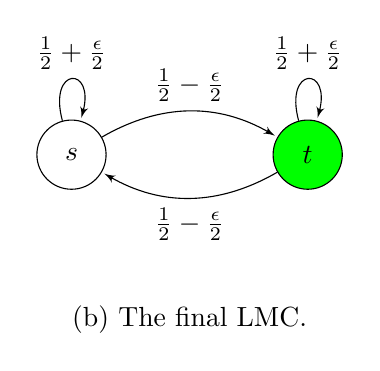
\begin{tikzpicture}[scale=.6,>=latex',shorten >=1pt,node distance=3cm,on grid,auto]

%\node[label]  at (2,2.7) {the MC~$\C$};

\node[state] (s) at (-1,0) {$s$};
\node[state, fill=green] (s2) at (4,0) {$t$};


%	\node[state] (u) at (19,0) {$u_1$};
%	\node[state, fill=green] (u2) at (24,0) {$u_2$};

\path[->] (s) edge [out=30,in=150] node [midway, above] {$\frac{1}{2}-\frac{\epsilon}{2}$} (s2);
\path[->] (s2) edge [out=210,in=-30] node [midway, below] {$\frac{1}{2}-\frac{\epsilon}{2}$} (s);

	\path[->] (s) edge [loop above]node [midway, above] {$\frac{1}{2} +\frac{\epsilon}{2}$} (s);
\path[->] (s2) edge [loop above] node [midway, above] {$\frac{1}{2} +\frac{\epsilon}{2} $} (s2);

\node at (1.5,-3.5) {(b) The final LMC.};
\end{tikzpicture}
%	\captionof{figure}{The final LMC.} \label{fig:example-intro-approximate-partition-refinement}
\end{minipage}
\caption{Example of running the minimisation algorithm using approximate partition refinement (Algorithm~\ref{alg:polynomial-optimistic-partition-refinement}) on the LMC in \cref{fig:intro3}.} \label{fig:example-intro-approximate-partition-refinement}
\end{figure}

%the approximate partition refinement
\paragraph*{Approximate Partition Refinement}
\begin{algorithm}[h]
	%		\setstretch{1.12}
	\DontPrintSemicolon
	\KwIn{An LMC $\Hyp = <S, L, \tauHyp, \ell>$, a compression parameter $\errorParam$}
	\KwOut{A partition $X$ over $S$}	
	$i := 0; X_0 := \{S\}$\;
	\Repeat{$X_i = X_{i-1}$}{
		$i := i+1$; $X_i := \emptyset$\;
		\ForEach{$E \in X_{i-1}$}{
			$X_E := \emptyset$\;
			%add $E': = \{s\}$ to $X_E$ where $s \in E$ \;		
			\For{$s \in E$}{
				$ESet := \{E'\in X_{E} \suchthat \text{for all } t\in E' \text{ we have } \ell(s)=\ell(t) \text{ and}\linebreak \|(\tauHyp(s)(E))_{E \in X_{i-1}} - (\tauHyp(t)(E))_{E \in X_{i-1}}\|_1 \le \epsilon_2 \}$\;
				\lIf{$ESet = \emptyset$}{
					$E': = \{s\}$
				}\Else{
					$E' := \arg\min\limits_{E' \in ESet}\big\{ \frac{\sum_{t \in  E'} \|(\tauHyp(s)(E))_{E \in X_{i-1}} - (\tauHyp(t)(E))_{E \in X_{i-1}}\|_1}{|E'|} \big\}$\;
					remove $E'$ from $X_E$; $E' := E' \cup \{ s \}$\;
				}
				add $E'$ to $X_E$ \;
			}
			$X_i := X_i \cup X_E$\;
		}
	}
	\caption{\mbox{Approximate Partition Refinement}}
	\label{alg:polynomial-optimistic-partition-refinement}
\end{algorithm}

Given a compression parameter $\epsilon_{2}$, the approximate partition refinement is shown in Algorithm~\ref{alg:polynomial-optimistic-partition-refinement}. At the beginning, an index $i$ is initialized to zero and we have $X_0 = \{S\}$, that is, all states are in the same set. In a refinement step, we increment $i$ and split each set $E \in X_{i-1}$ into one or more sets. We iterate though all $E \in X_{i-1}$ and for each $E$ we construct a set $X_E$, a partition of $E$. Starting with $X_E = \emptyset$, we iterate over all $s \in E$ (line~6). After each iteration, the current $s \in E$ appears in one set in $X_E$: either as a singleton or as an additional state in an already existing set in $X_E$. We give more details on this loop (lines~6-14) below.
After having partitioned~$E$ into~$X_E$, we add all sets in~$X_E$ to the new partition~$X_i$.
The way we split the sets ensures that for any two states from the same set in~$X_i$ the $L_1$-distance between the successor distributions over $X_{i-1}$ is at most $\epsilon_2$. The algorithm terminates when no splitting can be done.
Let $X$ be the final partition produced by the approximate partition refinement. For any two states $s, t \in E$ where $E \in X$, we have $\ell(s) = \ell(t)$ and $\|(\tauHyp(s)(E'))_{E' \in X} - (\tauHyp(t)(E'))_{E' \in X}\|_1 \le \epsilon_2$.

Let us give more details on the loop (lines~6-14) that partitions an $E \in X_i$.
For a state $s \in E$, a candidate set $\mathit{ESet}$ is computed such that for all $E' \in \mathit{ESet}$ the state $s$ and all $x \in E'$ have the same label and the $L_1$-distance between the successor distributions over $X_{i-1}$ of $s$ and any $x \in E'$ is at most $\epsilon_2$ (line~7). If $\mathit{ESet}$ is empty, we add the singleton $\{s\}$ into $X_E$ (line~8 and~13). If there is only one set $E'$ in $\mathit{ESet}$, we add $s$ to the set $E'$. Otherwise, if there are multiple elements in $\mathit{ESet}$ that satisfy the condition, we select the one as $E'$ such that the average $L_1$-distance between the successor distributions of $s$ and $x \in E'$ is the smallest (line~10). We add $s$ to the selected set $E'$ and include $E'$ in $X_{E}$ (line~10-13).


%which is also a set of $X_E$ by adding $s$

%If such $\mathit{ESet}$ is not empty, we select a set $E'$ from $\mathit{ESet}$ such that the average $L_1$-distance between $s$ and $x \in E'$ is the smallest (line~12). We then update $E'$ which is also a set of $X_E$ by adding $s$ (line~13-16).

\paragraph*{Minimisation Algorithm Using Approximate Partition Refinement}


\begin{algorithm}[h]
	\DontPrintSemicolon
	\KwIn{An LMC $\Hyp = <S, L, \tauHyp, \ell>$, a compression parameter $\epsilon_2$}
	\KwOut{An LMC $\Q_{i}$}
	$i := 0$\\
	%$\M^{i}: = <S, L, \tau', \ell>$ \\	
	%Compute $\sim_{\Hyp}$\\
	$\Q_{i} := \M_{i}/_{\sim_{\M_{i}}}$ where $\M_{i} = \Hyp$ and $\Q_{i} = <S^{\Q_{i}}, L, \tau^{\Q_{i}}, \ell^{\Q_{i}}>$ \;
	%$\omega' = \omega$\\
	%$d_{u, v} = 0 \forall u, v$ \\
	\Repeat{$|S^{\Q_{i}}| = |S^{\Q_{i-1}}|$}{
		Compute $X_i$ by running Algorithm~\ref{alg:polynomial-optimistic-partition-refinement} with $\Q_{i} $ and $\epsilon_2$ as input\;
		Construct an LMC $\M_{i+1} :=  <X_i, L , \tau^{\M_{i+1}}, \ell^{\M_{i+1}} >$ from $\Q_i$ where $\tau^{\M_{i+1}}(E) := \sum_{u \in  E}  \frac{(\tau^{\Q_{i}}(u)(E'))_{E' \in X_i}}{|E|}$ and $\ell^{\M_{i+1}}(E) := \ell^{\Q_{i}}(x)$ for all $E \in X_i$ and any $x \in E$\;
		% such that $\M_{i+1} :=  <X_i, L , \tau^{\M_{i+1}}, \ell^{\M_{i+1}} >$
		%		\ForEach{$x \in S^{\Hyp^{i-1}}$}{
		%			$\gamma_x := \sum_{u \in  E_x} \frac{(\tau^{\Hyp^{i-1}}(u)(E))_{E \in X}}{|E_x|}$ where $x \in E_x$ and $E_x \in X$\;
		%			$\nu_x$ is obtained by running \cref{alg:adjust-transition-probability} with $X$, $\tau^{\Hyp^{i-1}}(x)$ and $\gamma_x$\;
		%			$\tau'(x) = \nu_x$ \;
		%		}
		%		$\M^{i}: = <S^{\Hyp^{i-1}}, L, \tau', \ell^{\Hyp^{i-1}}>$\;
		%		$\Hyp^{i} :=\M^{i} / \sim_{\M^{i}}$ and $\Hyp^{i} = <S^{\Hyp^{i}}, L, \tau^{\Hyp^{i}}, \ell^{\Hyp^{i}}>$ \;
		%Obtain the new approximate quotient $\Q_{i+1}$ by exact quotienting $\M_{i+1}$, that is,
		$\Q_{i+1} := \M_{i+1} /_{\sim_{\M_{i+1}}}$\;
		$i := i+1$ \;
	}
	\caption{LMC Minimisation by Approximate Partition Refinement}
	\label{alg:approximate-partition-refinement-merge-algorithm}
\end{algorithm}

The minimisation algorithm using approximate partition refinement is shown in \cref{alg:approximate-partition-refinement-merge-algorithm}. The input is the same as the first minimisation algorithm: an LMC $\Hyp$ and a compression parameter $\epsilon_2$. An index $i$ is initialised to $0$. Similar to the approximate minimisation algorithm using local bisimilarity distances, we also start by computing the quotient LMC $\Q_{0} = \Hyp/_{\sim_{\Hyp}}$. It then steps into a loop. We compute the approximate partition $X_i$ of $\Q_{i}$ on line~4 and construct a new LMC $\M_{i+1}$ by setting $X_i$ as its state space on line~5. For any state $E \in X_i$, we set the probability distribution as the average probability distribution over $X_i$ from all $u \in E$. The label of any $E \in X$ is set to $\ell^{\Q_{i}}(u)$ where $u$ can be any state from $E$. A new approximate quotient $\Q_{i+1} $ is obtained by taking the exact quotient of $\M_{i+1}$. We increment $i$ at the end of the iteration and continue another iteration if the size of the state space of the new approximate quotient decreases. Otherwise, the algorithm terminates as we have no states to merge. As there are finitely many states, the algorithm always terminates.

%On line~5-10, we construct a new transition function $\tau'$ as described by \cref{proposition:transition-function-small-difference} and obtain a new LMC $\M^{i}$ by using $\tau'$ as its transition function.


Let $i \in \nat$. The following theorem applies to both the LMCs $\Q_{i}$ from \cref{alg:local-distance-merge-algorithm} and those from \cref{alg:approximate-partition-refinement-merge-algorithm}.
\begin{restatable}{theorem}{theoremBoundGlobalDistanceApproximatePartitionRefinement}\label{theorem:bounding-global-distance}
 %Let $d_{\glob}^{\M \oplus \Hyp} (x, x') \le \epsilon$ for all state $x$ in $\M$ and the corresponding state $x'$ in $\Hyp$.
 For all $i \in \nat$, we have that $\Q_{i+1}$ is an $\epsilon_2$-quotient of $\Q_i$. Furthermore, by the additivity lemma, we have that $\Q_i$ is an $i\epsilon_2$-quotient of $\Hyp$. %$d_{\glob}^{\Hyp^{0} \oplus \Hyp^{i}} (x, x_i) \le i \epsilon_2$ where $x$ is a state from $\Hyp^{0}$ and $x_i$ is the corresponding state in $\Hyp^{i}$.
\end{restatable}

In the case that $\Hyp=<S, L, \tauHyp, \ell>$ is a slightly perturbed version of $\M = <S, L,\tau,\ell>$, that is, for all $s \in S$ we have $\|\tau(s) - \tauHyp(s)\|_1 \le \epsilon$, the following corollary holds:
\begin{restatable}{corollary}{corollaryBoundQuotientError}\label{corollary:bounding-quotient-error}
 For all $i \in \nat$, we have that $\Q_i$ is an $(\epsilon + i\epsilon_2)$-quotient of $\M$.
\end{restatable}

 %with possibly imprecise transition probabilities.
%Let $\epsilon \gr 0$ be an error parameter. By slightly perturbed we mean that for each state the successor distributions in $\M_\epsilon$ and~$\M$ have small $L_1$-distance, i.e., at most $\epsilon$.	
%Since we have $R_{\epsilon} \subseteq \mathord{\sim_{\epsilon}}$ by \cref{proposition:approximate-global-relation-subset}, it follows from \cref{theorem:bounding-global-distance} that for all $i \in \nat$, $x \mathord{\sim_{i \epsilon_2}} x_i$ where $x$ is a state from $\Hyp^{0}$ and $x_i$ is the corresponding state in $\Hyp^{i}$.



\section{Active LMC Learning}
\label{section:active-LMC-learning}
%SETUP
%\begin{figure}[h]
%	\centering
%	
%	\begin{tikzpicture}[xscale=.6,>=latex',shorten >=1pt,node distance=3cm,on grid,auto]
%	
%	\node[label] (M) at (0,0) {$\M$};
%	\node[label] (Me) at (6,0) {$\Hyp$};
%	\node[label] (Meq) at (12,0) {$\Q_{0}$};
%	\node[label] (MOut) at (18,0) {$\Q_{i}$};
%	
%	\path[->] (M) edge node [midway, above] {perturbation} (Me);
%	\path[->] (M) edge node [midway, below] {(e.g., sampling)} (Me);
%	\path[->] (Me) edge node [midway, above] {exact quotient} (Meq);		
%	\path[->] (Meq) edge node [midway, above] {approximate} (MOut);		
%	\path[->] (Meq) edge node [midway, below] {minimisation} (MOut);				
%	\end{tikzpicture}
%	\caption{Workflow. \cref{lemma:additivity-property} is applied to $\M$, $\Q_{0}$ and $\Q_{i}$.}\label{fig:workflow}
%\end{figure}

%\subsection{Overall Approach}\label{subsection:learning-overall-approach}
%TODO In the first one (say "4A" for now), we describe our overall approach. I think we should say that we have an imprecise version of a (usually unknown) system. These two systems have small distance. For example, with sampling we can get this distance small with a high probability. (Notice that "high probability" only makes sense in the sampling context, not in general.) We also put the description of sampling in Section 4A.

%Let us assume that we do not have access to the transition probabilities of an LMC~$\M$. Rather, we have a slightly perturbed version $\Hyp=<S, L, \tauHyp, \ell>$ of $\M$. %with possibly imprecise transition probabilities.
%Let $\epsilon \gr 0$ be an error parameter. By slightly perturbed we mean that for each state the successor distributions in $\M_\epsilon$ and~$\M$ have small $L_1$-distance, i.e., at most $\epsilon$. For example, with sampling we can obtain with high probability a perturbed system that has small distance with $\M$.
%
%%TODO Then, still in 4A, we say that in the next section, say "4B" for now, we will present approximate minimisation algorithms. They produce a minimised system (i.e., a 3rd system) which has small distance from the perturbed system. We might give forward references to the theorems in 4B that claim this small distance.
%
%To compute an approximate quotient system of $\Hyp$, our first idea is to compute and merge states with small global bisimilarity distances. As it is $\sf NP$-complete to compute the global bisimilarity distances by \cref{theorem: global-epsilon-bisimulation-NP-complete}, this approach is not straightforward. Instead, in \cref{section:minimisation-algorithms}, we present two polynomial-time approximate minimisation algorithms. These two algorithms start by computing an LMC $\Hyp^{0}$, the exact quotient of $\Hyp$. With a compression parameter $\epsilon_2$ as input, they produce a minimised system $\Hyp^{i}$ where $i$ is the number of loop iterations of the two minimisation algorithms, respectively. From \cref{theorem:bounding-global-distance}, $\Hyp^{i}$ has global bisimilarity distance at most $i\epsilon_2$ from $\Hyp^{0}$, the exact quotient of the perturbed system.
%
%Together with the fact that $\M$ and $\Hyp$ (or its exact quotient $\Hyp^{0}$) have global bisimilarity distance at most $\epsilon$, it follows from \cref{lemma:additivity-property} that the minimised system $\Hyp^{i}$ and $\M$ have small global bisimilarity distance $\epsilon + i\epsilon_2$. \cref{fig:workflow} shows the workflow of our approach.

%TODO Then, still in 4A, we say that putting these two things together, by the triangle inequality (does it hold?), it follows that the unknown system has small distance to the minimised one. This holds with high probability if the imprecise chain has been obtained by sampling, and I think we can state that as a corollary (of the sampling theorem and the forward references).


%Let $\epsilon \gr 0$ be an error parameter and $\delta \gr 0$ be an error bound. Given a labelled Markov chain~$\M$ with possibly imprecise transition probabilities and a slightly perturbed version $\Hyp=<S, L, \tauHyp, \ell>$ of $\M$,  we hope to compute a compressed version of $\M$. By slightly perturbed we mean that for each state the successor distributions in $\Hyp$ and~$\M$ have $L_1$-distance which is at most~$\epsilon$ with probability at least $1 - \delta$. Next, we present how to obtain such approximation LMC by sampling.

%Our first idea is to merge states which have small global bisimilarity distances. However, as we have shown in \cref{theorem: global-epsilon-bisimulation-NP-complete} that it is $\sf NP$-complete to decide the global $\epsilon$-bisimulation, directly computing the global bisimilarity distances is highly inefficient. Alternatively, in \cref{subsection:local-bisimilarity-distances}, we provide a polynomial-time algorithm to compute an upper bound of the global bisimilarity distance. We can then merge the states for which this upper bound is small. In \cref{subsection:approximate-partition-refinement}, we introduce an approximate partition refinement, a polynomial algorithm similar to the exact partition refinement, which guarantees that states in an equivalence class of the final partition have small global bisimilarity distances and thus can be merged.

%\paragraph*{Approximation LMC by Sampling} \label{subsubsection:sampling}
We apply our approximate minimisation algorithms in a setting of active learning. Before that, we first describe how to obtain a perturbed LMC $\Hyp$ by sampling. Assume that we want to learn the transition probabilities of an LMC $\M$, that is, the state space, the labelling and the transitions are known. We also assume the system under learning (SUL) $\M$ could answer the query $\nxt$ which takes a state $s$ as input and returns a successor state of $s$ according to the transition probability distribution $\tau(s)$.

%Sampling
%We can approximate the transition probabilities via sampling.
Given a state $s$ of the LMC. We denote by $x_s$ the number of successor states of $s$ and by~$n_s$ the number of times we query the SUL on $\nxt(s)$. Let $N_{s,t}$ be the frequency counts of the query result $t$, that is, the number of times a successor state $t$ appears as the result returned by the queries. We approximate the transition probability distribution by $\tauHyp(s)$ where $\tauHyp(s)(t) = \frac{N_{s, t}}{n_s}$ for all successor states $t$ of $s$. (Such an estimator is called an empirical estimator in the literature.)

Intuitively, the more queries we ask the SUL, the more accurate the approximate probability distribution $\tauHyp(s)$ would be. In fact, the following theorem holds~\cite[Section~6.4]{BazilleGenestJegourelSun2020},~\cite{Chen2015}.

\begin{theorem}\label{theorem:sampling-size} Let $\epsilon \gr 0$ be an error parameter and $\delta \gr 0$ be an error bound. Let $s \in S$. We have $\Pr(\|\tau(s) - \tauHyp(s)\|_1 \le \epsilon) \ge 1 -\delta$ for $n_s \ge \frac{1}{2 \epsilon^{2}}\ln(\frac{2x_s}{\delta})$.
\end{theorem}

%Equivalently, for any $s \in S$, we have $\Pr(|\tau(s) - \tauHyp(s)| \le \epsilon) \ge (1-\delta)$ for $n_s \ge \frac{1}{2 \epsilon^{2}}\ln(\frac{2x_s}{\delta})$.
For each state $s \in S$, we query the SUL on $\nxt(s)$ for $n_s \ge \frac{1}{2 \epsilon^{2}}\ln(\frac{2x_s}{\delta})$ times. We can make $\delta$ small since it appears in the logarithmic term. We then approximate the transition function by $\tauHyp$ and construct a hypothesis LMC $\Hyp = <S, L, \tauHyp, \ell>$. Since the queries $\nxt(s)$ and $\nxt(t)$ for all $s,t \in S$ and $s \not= t$ are mutually independent, by Theorem~\ref{theorem:sampling-size}, we have that $\Pr(\forall s\in S: \|\tau(s) - \tauHyp(s)\|_1 \le \epsilon) \ge (1-\delta)^{|S|} $.
%%make delta small as it is in log

We then apply the minimisation algorithms with compression parameter $\epsilon_2$ on $\Hyp$ and obtain a minimised system $\Q_{i}$ which is an $i\epsilon_2$-quotient of $\Hyp$, the LMC constructed by sampling. Since with high probability the LMC $\Hyp$ (or its exact quotient $\Q_{0}$) has small distance $\epsilon$ with the SUL $\M$, it follows from \cref{corollary:bounding-quotient-error} that with high probability the minimised system $\Q_{i}$ is an $\epsilon'$-quotient of $\M$ where $\epsilon'$ is small:  for all $i \in \nat$, we have $\Pr(\Q_i \text{ is an }\epsilon'\text{-quotient of } \M \text{ with } \epsilon' \le \epsilon + i \epsilon_2) \ge (1-\delta)^{|S|}$. The probability does not come from our minimisation algorithms and depends solely on the sampling procedure.% and \cref{theorem:bounding-global-distance} holds that $\Q_i$ is an $i \epsilon_2$-quotient of $\Hyp$ for all $i \in \nat$.

%\cancel{
%	\begin{restatable}{corollary}{corollaryBoundGlobalDistance}\label{corollary:bounding-global-distance}
%		For all $i \in \nat$, we have $\Pr(d_{\glob}^{\M \oplus \Hyp^{i}} (x, x_i) \le \epsilon + i \epsilon_2) \ge (1-\delta)^{|S|}$ where $x$ is a state from the SUL $\M$ and $x_i$ is the corresponding state in $\Hyp^{i}$.
%	\end{restatable}
%}
%Assume we have constructed a hypothesis LMC  $\Hyp = <S, L, \tauHyp, \ell>$.

%After a hypothesis LMC  $\Hyp$ has been constructed, suppose we want to minimise $\Hyp$ such that with high probability the difference between the new LMC after minimisation and the SUL is small. We use the global bisimilarity distance to measure the difference between the hypothesis LMC and the SUL. It suffices to compute and merge states with small global bisimilarity distances. As it is $\sf NP$-complete to compute the global bisimilarity distances by \cref{theorem: global-epsilon-bisimulation-NP-complete}, it is not straightforward. Instead, we propose two polynomial-time algorithms to minimise the hypothesis LMC.




\section{Experiments}
\label{section:experiments}
In this section, we evaluate the performance of approximate minimisation algorithms on a number of LMCs. These LMCs model randomised algorithms and probabilistic protocols that are part of the probabilistic model checker PRISM \cite{KNP11}. The LMCs we run experiments on have less than $100,000$ states and model the following protocols or randomised algorithms: Herman's self-stabilisation algorithm \cite{Her90}, the synchronous leader election protocol by Itai and Rodeh \cite{ItaiR90}, the bounded retransmission protocol \cite{DarhenioJJL01}, the Crowds protocol \cite{ReiterR98} and the contract signing protocol by Even, Goldreich and Lempel \cite{EvenGL85}.

We implemented algorithms to obtain the slightly perturbed LMCs $\Hyp$. We call LMCs with fewer than $300$ states small; otherwise we call them large. For small LMCs, we sample the successor distribution for each state and obtain an approximation of it with error parameter $\epsilon$ and error bound $\delta$. For large LMCs, sampling is not practical as the sample size required by \cref{theorem:sampling-size} is very large. For these LMCs, we perturb the successor distribution by adding small noise to the successor transition probabilities so that for each state with at least probability $1-\delta$ the $L_1$-distance of the successor distributions in the perturbed and unperturbed systems is at most $\epsilon$ and otherwise the $L_1$-distance is $2\epsilon$. We vary the error parameter $\epsilon$ in the range of $\{0.00001, 0.0001, 0.001, 0.01\}$ and fix the error bound $\delta = 0.01$. For each unperturbed LMC and a pair of $\epsilon$ and $\delta$, we generate $5$ perturbed LMCs.

We also implemented the two minimisation algorithms in Java: \cref{alg:local-distance-merge-algorithm} and \cref{alg:approximate-partition-refinement-merge-algorithm}. The source code is publicly available\footnote{\url{https://github.com/qiyitang71/approximate-quotienting}}. We show some representative results in \cref{appendix:more-results}. The full experimental results are publicly available\footnote{\url{https://bit.ly/3vcpblY}}.

\begin{table}[t]
\begin{tabularx}{\textwidth}{@{}X@{}X@{}}
	\noindent\begin{tabular}{|c|c|c|c|}
			\hline %\\$\epsilon = 0.0001$
			\multirow{1}{*}{\shortstack[l]{Herman5}}&
			\# states&	\# trans&	\# iter\\
			\hline 						
			$\M$ \& $\Hyp$	&		 		32	  &			244				&\\
			$\M/_{\sim_{\M}}$	&		 		4	  &			11				&\\		
			$\Hyp/_{\sim_{\Hyp}}$      & 		23  &	       167             & \\
			\hline
			\multicolumn{4}{|c|}{Perturbed LMC \#1}\\
			\hline
			\multicolumn{4}{|c|}{$\epsilon_2 = 0.00001$}\\
			\hline
			local \& apr     & 23 & 167 & 0  \\
			%apr		  & 23 & 167 & 0  \\
			\hline
			\multicolumn{4}{|c|}{$\epsilon_2 = 0.0001$}\\
			\hline
			local \& apr     & 22 & 143 & 1  \\
			%apr		  & 22 & 143 & 1  \\
			\hline
			\multicolumn{4}{|c|}{$\epsilon_2 \in \{0.001, 0.01, 0.1\}$}\\
			\hline
			local    & 22 & 143 & 1    \\
			\rowcolor{yellow}
			apr		   & 4 & 11 & 1   \\
			\hline
			\rowcolor{white}
			\multicolumn{4}{c}{}\\			
		\end{tabular}
	~
		\noindent\begin{tabular}{|c|c|c|c|}
		\hline
		\multirow{1}{*}{\shortstack[l]{BRP32-2%\\$\epsilon = 0.0001$
		}} &
		\# states&	\# trans&	\# iter\\
		\hline
		$\M$ \& $\Hyp$ &	1349	 &			1731    & \\
		$\M/_{\sim_{\M}}$	&		 		647	  &			903				&\\								
		$\Hyp/_{\sim_{\Hyp}}$     & 		961	   & 	   	  1343        & \\
		\hline
		\multicolumn{4}{|c|}{Perturbed LMC \#1}\\
		\hline
		\multicolumn{4}{|c|}{$\epsilon_2 = 0.00001$}\\
		\hline
		apr		&   879 & 1230 & 2 \\
		\hline
		\multicolumn{4}{|c|}{$\epsilon_2 =  0.0001$}\\
		\hline
		apr		 &  705 & 986 & 2 \\
		\hline
		\multicolumn{4}{|c|}{$\epsilon_2 \in \{0.001, 0.01\}$}\\
		\hline
		\rowcolor{yellow}
		apr		 &  647 & 903 & 1\\
		\rowcolor{white}
		\hline
		\multicolumn{4}{|c|}{$\epsilon_2 = 0.1$}\\
		\hline
		\rowcolor{red!40}
		apr		 & 196  & 387 & 1 \\
		\hline
%		\rowcolor{white}
%		\multicolumn{4}{c}{}\\
	\end{tabular}	
\end{tabularx}
\caption{In the tables, local and apr stand for the minimisation algorithms using local bisimilarity distance and approximate partition refinement, respectively. The tables show the results for the first perturbed LMC (labeled with \#1) among the five perturbed LMCs generated by sampling or perturbing with $\epsilon =  0.0001$. (Left) Results of running the two minimisation algorithms on the LMC that models Herman's self-stabilisation algorithm with $5$ processes. (Right) Results of running apr on the LMC that models the bounded retransmission protocol with $N =32$ and $\mathit{MAX} = 2$. } \label{table:results}%\belowcaptionskip
\end{table}


%Due to the page limit, we only show partial results.

For the small LMCs, we apply both approximate minimisation algorithms to the perturbed LMCs with $\epsilon_2 \in \{0.00001, 0.0001, 0.001, 0.01, 0.1\}$. The results for a small LMC which models the Herman's self-stabilisation algorithm is shown on the left of \cref{table:results}. For the large LMCs, we only apply the approximate minimisation algorithm using approximate partition refinement to the perturbed LMCs, since the other minimisation algorithm could not finish on the large LMCs with timeout of two hours. The results for a large LMC which models the bounded retransmission protocol is shown on the right of \cref{table:results}.   %The rows are highlighted in red when $\epsilon_2$ is too big, i.e, the minimisation algorithms wrongly merge some states in the quotient of the original model. %when the structure of the quotient of the original model is successfully recovered.

For almost all models, given a perturbed LMC, we are able to recover the structure of the quotient of the unperturbed LMC when $\epsilon_2$ is appropriately chosen, that is, $\epsilon_2$ is no less than $\epsilon$ and is not too big; for example, see \cref{table:results} where the rows are highlighted in yellow. However, when $\epsilon_2$ is too big, the approximate minimisation algorithms may aggressively merge some states in the perturbed LMC and result in a quotient \modify{whose size is even smaller than that of the quotient of the unperturbed LMC}, as highlighted in red in \cref{table:results}. Also, we find that,  as expected, the exact partition refinement in general could not recover the structure of quotient of the original LMCs, except for the LMCs which model the synchronous leader election protocol by Itai and Rodeh. Furthermore, compared to the other approximate minimisation algorithm using the local bisimilarity distance, the one using approximate partition refinement performs much better in terms of running time and the ability to recover the structure of the quotient of the original model.

%The rows are highlighted in yellow when the structure of the quotient of the original model is successfully recovered. The rows are highlighted in red when $\epsilon_2$ is too big, i.e, the minimisation algorithms wrongly merge some states in the quotient of the original model.



One might ask whether the minimisation algorithm using approximate partition refinement always performs better than the one using the local bisimilarity distances. \modify{In general, this is not the case as shown by \cref{example:local-merging-better}. %in the appendix.

\begin{example}\label{example:local-merging-better}	
	Consider the LMC $\M = <S, L, \tau, \ell>$ shown in \cref{fig:example-local-merging-better}. Let $\epsilon_2 = 0.1$. First, we run Algorithm~\ref{alg:local-distance-merge-algorithm}. It proceeds in two iterations. In the first iteration, it computes the local bisimilarity distances for all pairs of states with the same label. We have $d_{\local}(s_1, s_2) = d_{\local}(s_2, s_3)= 0.54$ and $d_{\local}(s_1, s_3) = 0.04$. It then selects the pair $s_1$ and $s_3$ of which the local bisimilarity distance is less than $\epsilon_2$ and is the smallest. These two states are merged into $s_{13}$ in the LMC shown on the left of \cref{fig:example-local-merging-better2}. In the second iteration, the only pair of states with the same label are $s_{13}$ and $s_2$. Since $d_{\local}(s_{13}, s_2) = 0.06 \le \epsilon_2$, they are merged and we arrive at the final LMC shown on the right of \cref{fig:example-local-merging-better2}.
	
	Next, we run \cref{alg:approximate-partition-refinement-merge-algorithm} with the same inputs. In the first iteration, we run approximate partition refinement on line~5 (\cref{alg:polynomial-optimistic-partition-refinement}) and present \cref{tab:example-approximate-partition-refinement} as the possible partitions of the algorithm. At the beginning of the approximate partition refinement, we have partition $X_0$ as all states are in the same set. The states are then split by the labels and we get partition $X_1$. Next, we work on the set $\{s_1, s_2, s_3\}$. Suppose that we see $s_1$ and $s_2$ before $s_3$. We have $s_1$ and $s_2$ remain together as $\|(\tau(s_1)(E))_{E \in X_1}  - (\tau(s_2)(E))_{E \in X_1}\|_1 = 0.08 \le \epsilon_2$. However, since $\|(\tau(s_3)(E))_{E \in X_1}  - (\tau(s_2)(E))_{E \in X_1}\|_1 = 0.16 \gr \epsilon_2$, we have $ESet = \emptyset$ for $s_3$ on line~9 of Algorithm~\ref{alg:polynomial-optimistic-partition-refinement} and it is split out. In the next iteration, since $\|(\tau(s_1)(E))_{E \in X_2}  - (\tau(s_2)(E))_{E \in X_2}\|_1 = 0.54 \gr \epsilon_2$, $\{s_1, s_2\}$ is split into two singleton sets. The final partition $X_3$ in which all sets are singletons suggests no merging can be done and we are left with the original LMC $\M$.
	
	This example also shows that the order of iterating through the states matters for the approximate partition refinement algorithm. Indeed, suppose we iterate though $s_1$ and $s_3$ before $s_2$ after arriving at the partition $X_1$, we will have \cref{tab:example-approximate-partition-refinement2} as the partitions and finally get the  LMC on the right of \cref{fig:example-local-merging-better2} just as the other minimisation algorithm. %. We can then merge $s_1$ and $s_3$ to get the LMC on the left of \cref{fig:example-local-merging-better2}. Moreover, we will proceed into running approximate partition refinement algorithm again and get the final LMC on the right of \cref{fig:example-local-merging-better2} just as the other minimisation algorithm.
	\qed
	
\end{example}
}

\begin{minipage}{0.5\textwidth}
	
	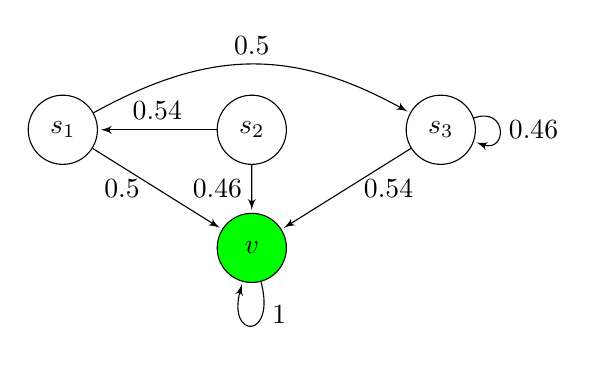
\begin{tikzpicture}[xscale=.6,>=latex',shorten >=1pt,node distance=3cm,on grid,auto]
	
	\node[state] (s) at (-6,0) {$s_1$};
	\node[state] (t) at (-2,0) {$s_2$};
	\node[state] (u) at (2,0) {$s_3$};
	\node[state, fill=green] (v) at (-2,-1.5) {$v$};
	
	\path[->] (s) edge [out=20,in=160] node [midway, above] {$0.5$} (u);
	\path[->] (s) edge node [midway, left, xshift=-0.1cm] {$0.5$} (v);
	
	\path[->] (t) edge node [midway, left] {$0.46$} (v);
	\path[->] (t) edge node [midway, above]  {$0.54$} (s);%[out=160,in=20]
	
	\path[->] (u) edge node [midway, right, xshift=0.1cm] {$0.54$} (v);
	\path[->] (u) edge [loop right] node [midway, right] {$0.46$} (u);
	
	\path[->] (v) edge [out=-70, in=-110, looseness=4] node [near start, right] {$1$} (v);
	\end{tikzpicture}
	\captionof{figure}{The LMC for which Algorithm~\ref{alg:local-distance-merge-algorithm} may perform better than Algorithm~\ref{alg:approximate-partition-refinement-merge-algorithm}.}
	\label{fig:example-local-merging-better}
\end{minipage}
\hfill
\begin{minipage}{0.45\textwidth}
	\centering	\vspace{0.1cm}
	\begin{tabular}{l}
		\\\\\\
		\hline%wd{0.5pt}
		$X_0 = \{S\}$ \\
		$X_1 = \big\{  \{s_1,s_2,s_3\} , \{v\} \big\}$\\
		$X_2 = \big\{  \{s_1, s_2\}, \{s_3\} , \{v\} \big\}$\\
		$X_3 = \big\{  \{s_1\},\{s_2\}, \{s_3\} , \{v\} \big\}$\\
		\hline
		\\\\
	\end{tabular}
	\captionof{table}{Example of running Algorithm~\ref{alg:polynomial-optimistic-partition-refinement} on the LMC in \cref{fig:example-local-merging-better}. (Suppose we iterate through $s_1$ and $s_2$ before $s_3$.)} \label{tab:example-approximate-partition-refinement}
\end{minipage}

\begin{minipage}{0.5\textwidth}
	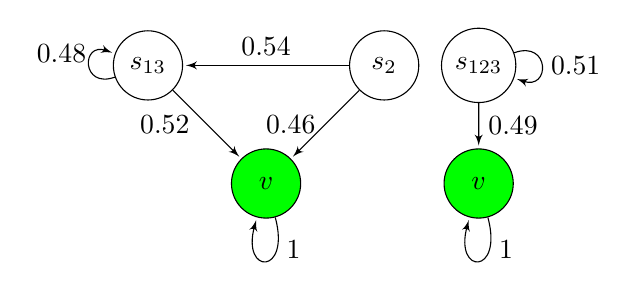
\begin{tikzpicture}[xscale=.6,>=latex',shorten >=1pt,node distance=3cm,on grid,auto]
	
	\node[state] (s13) at (1.5,0) {$s_{13}$};
	\node[state] (s2) at (6.5,0) {$s_2$};
	\node[state, fill=green] (v1) at (4,-1.5) {$v$};
	
	\path[->] (s13) edge node [midway, left, xshift=-0.1cm] {$0.52$} (v1);
	\path[->] (s13) edge [loop left] node [near end, left] {$0.48$} (s13);
	
	\path[->] (s2) edge node [midway, left] {$0.46$} (v1);
	\path[->] (s2) edge node [midway, above]  {$0.54$} (s13);
	
	\path[->] (v1) edge [out=-70, in=-110, looseness=4] node [near start, right] {$1$} (v1);
	
	\node[state] (ss) at (8.5,0) {$s_{123}$};
	\node[state, fill=green] (vv) at (8.5,-1.5) {$v$};
	
	\path[->] (ss) edge node [midway, right] {$0.49$} (vv);
	\path[->] (ss) edge [loop right] node [midway, right] {$0.51$} (ss);
	\path[->] (vv) edge [out=-70, in=-110, looseness=4] node [near start, right] {$1$} (vv);
	
	\end{tikzpicture}
	\captionof{figure}{Two Steps of Running Algorithm~\ref{alg:local-distance-merge-algorithm}.}\label{fig:example-local-merging-better2}
\end{minipage}
\hfill
\begin{minipage}{0.45\textwidth}
	\centering\vspace{0.2cm}
	\begin{tabular}{l}
		\\\\
		\hline%wd{0.5pt}
		$X_0 = \{S\}$ \\
		$X_1 = \big\{  \{s_1,s_3,s_2\} , \{v\} \big\}$\\
		$X_2 = \big\{  \{s_1, s_3\}, \{s_2\} , \{v\} \big\}$\\
		\hline
		\\
	\end{tabular}
	\captionof{table}{Example of running Algorithm~\ref{alg:polynomial-optimistic-partition-refinement} on the LMC in \cref{fig:example-local-merging-better}. (Suppose we iterate through $s_1$ and $s_3$ before $s_2$.)} \label{tab:example-approximate-partition-refinement2}
\end{minipage}


\section{Conclusion}\label{section:conclusion}

We have developed and analysed algorithms for minimising probabilistic systems via approximate bisimulation.
These algorithms are based on $\epsilon$-quotients, a novel yet natural notion of approximate quotients.
We have obtained theoretical bounds on the discrepancy between the minimised and the non-minimised systems.
In our experiments, approximate partition refinement does well in minimising labelled Markov chains with perturbed  transition probabilities,
suggesting that approximate partition refinement is a practical approach for ``recognising'' and exploiting approximate bisimulation.

Future work might consider the following questions: Does approximate minimisation allow for further forms of active learning? Can our techniques be transferred to Markov decision processes?

\bibliography{paper}

\newpage\appendix\label{section:appendix}
\chapter{Supplementary Material}
\label{appendix}

In this appendix, we present supplementary material for the techniques and
experiments presented in the main text.

\section{Baseline Results and Analysis for Informed Sampler}
\label{appendix:chap3}

Here, we give an in-depth
performance analysis of the various samplers and the effect of their
hyperparameters. We choose hyperparameters with the lowest PSRF value
after $10k$ iterations, for each sampler individually. If the
differences between PSRF are not significantly different among
multiple values, we choose the one that has the highest acceptance
rate.

\subsection{Experiment: Estimating Camera Extrinsics}
\label{appendix:chap3:room}

\subsubsection{Parameter Selection}
\paragraph{Metropolis Hastings (\MH)}

Figure~\ref{fig:exp1_MH} shows the median acceptance rates and PSRF
values corresponding to various proposal standard deviations of plain
\MH~sampling. Mixing gets better and the acceptance rate gets worse as
the standard deviation increases. The value $0.3$ is selected standard
deviation for this sampler.

\paragraph{Metropolis Hastings Within Gibbs (\MHWG)}

As mentioned in Section~\ref{sec:room}, the \MHWG~sampler with one-dimensional
updates did not converge for any value of proposal standard deviation.
This problem has high correlation of the camera parameters and is of
multi-modal nature, which this sampler has problems with.

\paragraph{Parallel Tempering (\PT)}

For \PT~sampling, we took the best performing \MH~sampler and used
different temperature chains to improve the mixing of the
sampler. Figure~\ref{fig:exp1_PT} shows the results corresponding to
different combination of temperature levels. The sampler with
temperature levels of $[1,3,27]$ performed best in terms of both
mixing and acceptance rate.

\paragraph{Effect of Mixture Coefficient in Informed Sampling (\MIXLMH)}

Figure~\ref{fig:exp1_alpha} shows the effect of mixture
coefficient ($\alpha$) on the informed sampling
\MIXLMH. Since there is no significant different in PSRF values for
$0 \le \alpha \le 0.7$, we chose $0.7$ due to its high acceptance
rate.


% \end{multicols}

\begin{figure}[h]
\centering
  \subfigure[MH]{%
    \includegraphics[width=.48\textwidth]{figures/supplementary/camPose_MH.pdf} \label{fig:exp1_MH}
  }
  \subfigure[PT]{%
    \includegraphics[width=.48\textwidth]{figures/supplementary/camPose_PT.pdf} \label{fig:exp1_PT}
  }
\\
  \subfigure[INF-MH]{%
    \includegraphics[width=.48\textwidth]{figures/supplementary/camPose_alpha.pdf} \label{fig:exp1_alpha}
  }
  \mycaption{Results of the `Estimating Camera Extrinsics' experiment}{PRSFs and Acceptance rates corresponding to (a) various standard deviations of \MH, (b) various temperature level combinations of \PT sampling and (c) various mixture coefficients of \MIXLMH sampling.}
\end{figure}



\begin{figure}[!t]
\centering
  \subfigure[\MH]{%
    \includegraphics[width=.48\textwidth]{figures/supplementary/occlusionExp_MH.pdf} \label{fig:exp2_MH}
  }
  \subfigure[\BMHWG]{%
    \includegraphics[width=.48\textwidth]{figures/supplementary/occlusionExp_BMHWG.pdf} \label{fig:exp2_BMHWG}
  }
\\
  \subfigure[\MHWG]{%
    \includegraphics[width=.48\textwidth]{figures/supplementary/occlusionExp_MHWG.pdf} \label{fig:exp2_MHWG}
  }
  \subfigure[\PT]{%
    \includegraphics[width=.48\textwidth]{figures/supplementary/occlusionExp_PT.pdf} \label{fig:exp2_PT}
  }
\\
  \subfigure[\INFBMHWG]{%
    \includegraphics[width=.5\textwidth]{figures/supplementary/occlusionExp_alpha.pdf} \label{fig:exp2_alpha}
  }
  \mycaption{Results of the `Occluding Tiles' experiment}{PRSF and
    Acceptance rates corresponding to various standard deviations of
    (a) \MH, (b) \BMHWG, (c) \MHWG, (d) various temperature level
    combinations of \PT~sampling and; (e) various mixture coefficients
    of our informed \INFBMHWG sampling.}
\end{figure}

%\onecolumn\newpage\twocolumn
\subsection{Experiment: Occluding Tiles}
\label{appendix:chap3:tiles}

\subsubsection{Parameter Selection}

\paragraph{Metropolis Hastings (\MH)}

Figure~\ref{fig:exp2_MH} shows the results of
\MH~sampling. Results show the poor convergence for all proposal
standard deviations and rapid decrease of AR with increasing standard
deviation. This is due to the high-dimensional nature of
the problem. We selected a standard deviation of $1.1$.

\paragraph{Blocked Metropolis Hastings Within Gibbs (\BMHWG)}

The results of \BMHWG are shown in Figure~\ref{fig:exp2_BMHWG}. In
this sampler we update only one block of tile variables (of dimension
four) in each sampling step. Results show much better performance
compared to plain \MH. The optimal proposal standard deviation for
this sampler is $0.7$.

\paragraph{Metropolis Hastings Within Gibbs (\MHWG)}

Figure~\ref{fig:exp2_MHWG} shows the result of \MHWG sampling. This
sampler is better than \BMHWG and converges much more quickly. Here
a standard deviation of $0.9$ is found to be best.

\paragraph{Parallel Tempering (\PT)}

Figure~\ref{fig:exp2_PT} shows the results of \PT sampling with various
temperature combinations. Results show no improvement in AR from plain
\MH sampling and again $[1,3,27]$ temperature levels are found to be optimal.

\paragraph{Effect of Mixture Coefficient in Informed Sampling (\INFBMHWG)}

Figure~\ref{fig:exp2_alpha} shows the effect of mixture
coefficient ($\alpha$) on the blocked informed sampling
\INFBMHWG. Since there is no significant different in PSRF values for
$0 \le \alpha \le 0.8$, we chose $0.8$ due to its high acceptance
rate.



\subsection{Experiment: Estimating Body Shape}
\label{appendix:chap3:body}

\subsubsection{Parameter Selection}
\paragraph{Metropolis Hastings (\MH)}

Figure~\ref{fig:exp3_MH} shows the result of \MH~sampling with various
proposal standard deviations. The value of $0.1$ is found to be
best.

\paragraph{Metropolis Hastings Within Gibbs (\MHWG)}

For \MHWG sampling we select $0.3$ proposal standard
deviation. Results are shown in Fig.~\ref{fig:exp3_MHWG}.


\paragraph{Parallel Tempering (\PT)}

As before, results in Fig.~\ref{fig:exp3_PT}, the temperature levels
were selected to be $[1,3,27]$ due its slightly higher AR.

\paragraph{Effect of Mixture Coefficient in Informed Sampling (\MIXLMH)}

Figure~\ref{fig:exp3_alpha} shows the effect of $\alpha$ on PSRF and
AR. Since there is no significant differences in PSRF values for $0 \le
\alpha \le 0.8$, we choose $0.8$.


\begin{figure}[t]
\centering
  \subfigure[\MH]{%
    \includegraphics[width=.48\textwidth]{figures/supplementary/bodyShape_MH.pdf} \label{fig:exp3_MH}
  }
  \subfigure[\MHWG]{%
    \includegraphics[width=.48\textwidth]{figures/supplementary/bodyShape_MHWG.pdf} \label{fig:exp3_MHWG}
  }
\\
  \subfigure[\PT]{%
    \includegraphics[width=.48\textwidth]{figures/supplementary/bodyShape_PT.pdf} \label{fig:exp3_PT}
  }
  \subfigure[\MIXLMH]{%
    \includegraphics[width=.48\textwidth]{figures/supplementary/bodyShape_alpha.pdf} \label{fig:exp3_alpha}
  }
\\
  \mycaption{Results of the `Body Shape Estimation' experiment}{PRSFs and
    Acceptance rates corresponding to various standard deviations of
    (a) \MH, (b) \MHWG; (c) various temperature level combinations
    of \PT sampling and; (d) various mixture coefficients of the
    informed \MIXLMH sampling.}
\end{figure}


\subsection{Results Overview}
Figure~\ref{fig:exp_summary} shows the summary results of the all the three
experimental studies related to informed sampler.
\begin{figure*}[h!]
\centering
  \subfigure[Results for: Estimating Camera Extrinsics]{%
    \includegraphics[width=0.9\textwidth]{figures/supplementary/camPose_ALL.pdf} \label{fig:exp1_all}
  }
  \subfigure[Results for: Occluding Tiles]{%
    \includegraphics[width=0.9\textwidth]{figures/supplementary/occlusionExp_ALL.pdf} \label{fig:exp2_all}
  }
  \subfigure[Results for: Estimating Body Shape]{%
    \includegraphics[width=0.9\textwidth]{figures/supplementary/bodyShape_ALL.pdf} \label{fig:exp3_all}
  }
  \label{fig:exp_summary}
  \mycaption{Summary of the statistics for the three experiments}{Shown are
    for several baseline methods and the informed samplers the
    acceptance rates (left), PSRFs (middle), and RMSE values
    (right). All results are median results over multiple test
    examples.}
\end{figure*}

\subsection{Additional Qualitative Results}

\subsubsection{Occluding Tiles}
In Figure~\ref{fig:exp2_visual_more} more qualitative results of the
occluding tiles experiment are shown. The informed sampling approach
(\INFBMHWG) is better than the best baseline (\MHWG). This still is a
very challenging problem since the parameters for occluded tiles are
flat over a large region. Some of the posterior variance of the
occluded tiles is already captured by the informed sampler.

\begin{figure*}[h!]
\begin{center}
\centerline{\includegraphics[width=0.95\textwidth]{figures/supplementary/occlusionExp_Visual.pdf}}
\mycaption{Additional qualitative results of the occluding tiles experiment}
  {From left to right: (a)
  Given image, (b) Ground truth tiles, (c) OpenCV heuristic and most probable estimates
  from 5000 samples obtained by (d) MHWG sampler (best baseline) and
  (e) our INF-BMHWG sampler. (f) Posterior expectation of the tiles
  boundaries obtained by INF-BMHWG sampling (First 2000 samples are
  discarded as burn-in).}
\label{fig:exp2_visual_more}
\end{center}
\end{figure*}

\subsubsection{Body Shape}
Figure~\ref{fig:exp3_bodyMeshes} shows some more results of 3D mesh
reconstruction using posterior samples obtained by our informed
sampling \MIXLMH.

\begin{figure*}[t]
\begin{center}
\centerline{\includegraphics[width=0.75\textwidth]{figures/supplementary/bodyMeshResults.pdf}}
\mycaption{Qualitative results for the body shape experiment}
  {Shown is the 3D mesh reconstruction results with first 1000 samples obtained
  using the \MIXLMH informed sampling method. (blue indicates small
  values and red indicates high values)}
\label{fig:exp3_bodyMeshes}
\end{center}
\end{figure*}

\clearpage



\section{Additional Results on the Face Problem with CMP}

Figure~\ref{fig:shading-qualitative-multiple-subjects-supp} shows inference results for reflectance maps, normal maps and lights for randomly chosen test images, and Fig.~\ref{fig:shading-qualitative-same-subject-supp} shows reflectance estimation results on multiple images of the same subject produced under different illumination conditions. CMP is able to produce estimates that are closer to the groundtruth across different subjects and illumination conditions.

\begin{figure*}[h]
  \begin{center}
  \centerline{\includegraphics[width=1.0\columnwidth]{figures/face_cmp_visual_results_supp.pdf}}
  \vspace{-1.2cm}
  \end{center}
	\mycaption{A visual comparison of inference results}{(a)~Observed images. (b)~Inferred reflectance maps. \textit{GT} is the photometric stereo groundtruth, \textit{BU} is the Biswas \etal (2009) reflectance estimate and \textit{Forest} is the consensus prediction. (c)~The variance of the inferred reflectance estimate produced by \MTD (normalized across rows).(d)~Visualization of inferred light directions. (e)~Inferred normal maps.}
	\label{fig:shading-qualitative-multiple-subjects-supp}
\end{figure*}


\begin{figure*}[h]
	\centering
	\setlength\fboxsep{0.2mm}
	\setlength\fboxrule{0pt}
	\begin{tikzpicture}

		\matrix at (0, 0) [matrix of nodes, nodes={anchor=east}, column sep=-0.05cm, row sep=-0.2cm]
		{
			\fbox{\includegraphics[width=1cm]{figures/sample_3_4_X.png}} &
			\fbox{\includegraphics[width=1cm]{figures/sample_3_4_GT.png}} &
			\fbox{\includegraphics[width=1cm]{figures/sample_3_4_BISWAS.png}}  &
			\fbox{\includegraphics[width=1cm]{figures/sample_3_4_VMP.png}}  &
			\fbox{\includegraphics[width=1cm]{figures/sample_3_4_FOREST.png}}  &
			\fbox{\includegraphics[width=1cm]{figures/sample_3_4_CMP.png}}  &
			\fbox{\includegraphics[width=1cm]{figures/sample_3_4_CMPVAR.png}}
			 \\

			\fbox{\includegraphics[width=1cm]{figures/sample_3_5_X.png}} &
			\fbox{\includegraphics[width=1cm]{figures/sample_3_5_GT.png}} &
			\fbox{\includegraphics[width=1cm]{figures/sample_3_5_BISWAS.png}}  &
			\fbox{\includegraphics[width=1cm]{figures/sample_3_5_VMP.png}}  &
			\fbox{\includegraphics[width=1cm]{figures/sample_3_5_FOREST.png}}  &
			\fbox{\includegraphics[width=1cm]{figures/sample_3_5_CMP.png}}  &
			\fbox{\includegraphics[width=1cm]{figures/sample_3_5_CMPVAR.png}}
			 \\

			\fbox{\includegraphics[width=1cm]{figures/sample_3_6_X.png}} &
			\fbox{\includegraphics[width=1cm]{figures/sample_3_6_GT.png}} &
			\fbox{\includegraphics[width=1cm]{figures/sample_3_6_BISWAS.png}}  &
			\fbox{\includegraphics[width=1cm]{figures/sample_3_6_VMP.png}}  &
			\fbox{\includegraphics[width=1cm]{figures/sample_3_6_FOREST.png}}  &
			\fbox{\includegraphics[width=1cm]{figures/sample_3_6_CMP.png}}  &
			\fbox{\includegraphics[width=1cm]{figures/sample_3_6_CMPVAR.png}}
			 \\
	     };

       \node at (-3.85, -2.0) {\small Observed};
       \node at (-2.55, -2.0) {\small `GT'};
       \node at (-1.27, -2.0) {\small BU};
       \node at (0.0, -2.0) {\small MP};
       \node at (1.27, -2.0) {\small Forest};
       \node at (2.55, -2.0) {\small \textbf{CMP}};
       \node at (3.85, -2.0) {\small Variance};

	\end{tikzpicture}
	\mycaption{Robustness to varying illumination}{Reflectance estimation on a subject images with varying illumination. Left to right: observed image, photometric stereo estimate (GT)
  which is used as a proxy for groundtruth, bottom-up estimate of \cite{Biswas2009}, VMP result, consensus forest estimate, CMP mean, and CMP variance.}
	\label{fig:shading-qualitative-same-subject-supp}
\end{figure*}

\clearpage

\section{Additional Material for Learning Sparse High Dimensional Filters}
\label{sec:appendix-bnn}

This part of supplementary material contains a more detailed overview of the permutohedral
lattice convolution in Section~\ref{sec:permconv}, more experiments in
Section~\ref{sec:addexps} and additional results with protocols for
the experiments presented in Chapter~\ref{chap:bnn} in Section~\ref{sec:addresults}.

\vspace{-0.2cm}
\subsection{General Permutohedral Convolutions}
\label{sec:permconv}

A core technical contribution of this work is the generalization of the Gaussian permutohedral lattice
convolution proposed in~\cite{adams2010fast} to the full non-separable case with the
ability to perform back-propagation. Although, conceptually, there are minor
differences between Gaussian and general parameterized filters, there are non-trivial practical
differences in terms of the algorithmic implementation. The Gauss filters belong to
the separable class and can thus be decomposed into multiple
sequential one dimensional convolutions. We are interested in the general filter
convolutions, which can not be decomposed. Thus, performing a general permutohedral
convolution at a lattice point requires the computation of the inner product with the
neighboring elements in all the directions in the high-dimensional space.

Here, we give more details of the implementation differences of separable
and non-separable filters. In the following, we will explain the scalar case first.
Recall, that the forward pass of general permutohedral convolution
involves 3 steps: \textit{splatting}, \textit{convolving} and \textit{slicing}.
We follow the same splatting and slicing strategies as in~\cite{adams2010fast}
since these operations do not depend on the filter kernel. The main difference
between our work and the existing implementation of~\cite{adams2010fast} is
the way that the convolution operation is executed. This proceeds by constructing
a \emph{blur neighbor} matrix $K$ that stores for every lattice point all
values of the lattice neighbors that are needed to compute the filter output.

\begin{figure}[t!]
  \centering
    \includegraphics[width=0.6\columnwidth]{figures/supplementary/lattice_construction}
  \mycaption{Illustration of 1D permutohedral lattice construction}
  {A $4\times 4$ $(x,y)$ grid lattice is projected onto the plane defined by the normal
  vector $(1,1)^{\top}$. This grid has $s+1=4$ and $d=2$ $(s+1)^{d}=4^2=16$ elements.
  In the projection, all points of the same color are projected onto the same points in the plane.
  The number of elements of the projected lattice is $t=(s+1)^d-s^d=4^2-3^2=7$, that is
  the $(4\times 4)$ grid minus the size of lattice that is $1$ smaller at each size, in this
  case a $(3\times 3)$ lattice (the upper right $(3\times 3)$ elements).
  }
\label{fig:latticeconstruction}
\end{figure}

The blur neighbor matrix is constructed by traversing through all the populated
lattice points and their neighboring elements.
% For efficiency, we do this matrix construction recursively with shared computations
% since $n^{th}$ neighbourhood elements are $1^{st}$ neighborhood elements of $n-1^{th}$ neighbourhood elements. \pg{do not understand}
This is done recursively to share computations. For any lattice point, the neighbors that are
$n$ hops away are the direct neighbors of the points that are $n-1$ hops away.
The size of a $d$ dimensional spatial filter with width $s+1$ is $(s+1)^{d}$ (\eg, a
$3\times 3$ filter, $s=2$ in $d=2$ has $3^2=9$ elements) and this size grows
exponentially in the number of dimensions $d$. The permutohedral lattice is constructed by
projecting a regular grid onto the plane spanned by the $d$ dimensional normal vector ${(1,\ldots,1)}^{\top}$. See
Fig.~\ref{fig:latticeconstruction} for an illustration of the 1D lattice construction.
Many corners of a grid filter are projected onto the same point, in total $t = {(s+1)}^{d} -
s^{d}$ elements remain in the permutohedral filter with $s$ neighborhood in $d-1$ dimensions.
If the lattice has $m$ populated elements, the
matrix $K$ has size $t\times m$. Note that, since the input signal is typically
sparse, only a few lattice corners are being populated in the \textit{slicing} step.
We use a hash-table to keep track of these points and traverse only through
the populated lattice points for this neighborhood matrix construction.

Once the blur neighbor matrix $K$ is constructed, we can perform the convolution
by the matrix vector multiplication
\begin{equation}
\ell' = BK,
\label{eq:conv}
\end{equation}
where $B$ is the $1 \times t$ filter kernel (whose values we will learn) and $\ell'\in\mathbb{R}^{1\times m}$
is the result of the filtering at the $m$ lattice points. In practice, we found that the
matrix $K$ is sometimes too large to fit into GPU memory and we divided the matrix $K$
into smaller pieces to compute Eq.~\ref{eq:conv} sequentially.

In the general multi-dimensional case, the signal $\ell$ is of $c$ dimensions. Then
the kernel $B$ is of size $c \times t$ and $K$ stores the $c$ dimensional vectors
accordingly. When the input and output points are different, we slice only the
input points and splat only at the output points.


\subsection{Additional Experiments}
\label{sec:addexps}
In this section, we discuss more use-cases for the learned bilateral filters, one
use-case of BNNs and two single filter applications for image and 3D mesh denoising.

\subsubsection{Recognition of subsampled MNIST}\label{sec:app_mnist}

One of the strengths of the proposed filter convolution is that it does not
require the input to lie on a regular grid. The only requirement is to define a distance
between features of the input signal.
We highlight this feature with the following experiment using the
classical MNIST ten class classification problem~\cite{lecun1998mnist}. We sample a
sparse set of $N$ points $(x,y)\in [0,1]\times [0,1]$
uniformly at random in the input image, use their interpolated values
as signal and the \emph{continuous} $(x,y)$ positions as features. This mimics
sub-sampling of a high-dimensional signal. To compare against a spatial convolution,
we interpolate the sparse set of values at the grid positions.

We take a reference implementation of LeNet~\cite{lecun1998gradient} that
is part of the Caffe project~\cite{jia2014caffe} and compare it
against the same architecture but replacing the first convolutional
layer with a bilateral convolution layer (BCL). The filter size
and numbers are adjusted to get a comparable number of parameters
($5\times 5$ for LeNet, $2$-neighborhood for BCL).

The results are shown in Table~\ref{tab:all-results}. We see that training
on the original MNIST data (column Original, LeNet vs. BNN) leads to a slight
decrease in performance of the BNN (99.03\%) compared to LeNet
(99.19\%). The BNN can be trained and evaluated on sparse
signals, and we resample the image as described above for $N=$ 100\%, 60\% and
20\% of the total number of pixels. The methods are also evaluated
on test images that are subsampled in the same way. Note that we can
train and test with different subsampling rates. We introduce an additional
bilinear interpolation layer for the LeNet architecture to train on the same
data. In essence, both models perform a spatial interpolation and thus we
expect them to yield a similar classification accuracy. Once the data is of
higher dimensions, the permutohedral convolution will be faster due to hashing
the sparse input points, as well as less memory demanding in comparison to
naive application of a spatial convolution with interpolated values.

\begin{table}[t]
  \begin{center}
    \footnotesize
    \centering
    \begin{tabular}[t]{lllll}
      \toprule
              &     & \multicolumn{3}{c}{Test Subsampling} \\
       Method  & Original & 100\% & 60\% & 20\%\\
      \midrule
       LeNet &  \textbf{0.9919} & 0.9660 & 0.9348 & \textbf{0.6434} \\
       BNN &  0.9903 & \textbf{0.9844} & \textbf{0.9534} & 0.5767 \\
      \hline
       LeNet 100\% & 0.9856 & 0.9809 & 0.9678 & \textbf{0.7386} \\
       BNN 100\% & \textbf{0.9900} & \textbf{0.9863} & \textbf{0.9699} & 0.6910 \\
      \hline
       LeNet 60\% & 0.9848 & 0.9821 & 0.9740 & 0.8151 \\
       BNN 60\% & \textbf{0.9885} & \textbf{0.9864} & \textbf{0.9771} & \textbf{0.8214}\\
      \hline
       LeNet 20\% & \textbf{0.9763} & \textbf{0.9754} & 0.9695 & 0.8928 \\
       BNN 20\% & 0.9728 & 0.9735 & \textbf{0.9701} & \textbf{0.9042}\\
      \bottomrule
    \end{tabular}
  \end{center}
\vspace{-.2cm}
\caption{Classification accuracy on MNIST. We compare the
    LeNet~\cite{lecun1998gradient} implementation that is part of
    Caffe~\cite{jia2014caffe} to the network with the first layer
    replaced by a bilateral convolution layer (BCL). Both are trained
    on the original image resolution (first two rows). Three more BNN
    and CNN models are trained with randomly subsampled images (100\%,
    60\% and 20\% of the pixels). An additional bilinear interpolation
    layer samples the input signal on a spatial grid for the CNN model.
  }
  \label{tab:all-results}
\vspace{-.5cm}
\end{table}

\subsubsection{Image Denoising}

The main application that inspired the development of the bilateral
filtering operation is image denoising~\cite{aurich1995non}, there
using a single Gaussian kernel. Our development allows to learn this
kernel function from data and we explore how to improve using a \emph{single}
but more general bilateral filter.

We use the Berkeley segmentation dataset
(BSDS500)~\cite{arbelaezi2011bsds500} as a test bed. The color
images in the dataset are converted to gray-scale,
and corrupted with Gaussian noise with a standard deviation of
$\frac {25} {255}$.

We compare the performance of four different filter models on a
denoising task.
The first baseline model (`Spatial' in Table \ref{tab:denoising}, $25$
weights) uses a single spatial filter with a kernel size of
$5$ and predicts the scalar gray-scale value at the center pixel. The next model
(`Gauss Bilateral') applies a bilateral \emph{Gaussian}
filter to the noisy input, using position and intensity features $\f=(x,y,v)^\top$.
The third setup (`Learned Bilateral', $65$ weights)
takes a Gauss kernel as initialization and
fits all filter weights on the train set to minimize the
mean squared error with respect to the clean images.
We run a combination
of spatial and permutohedral convolutions on spatial and bilateral
features (`Spatial + Bilateral (Learned)') to check for a complementary
performance of the two convolutions.

\label{sec:exp:denoising}
\begin{table}[!h]
\begin{center}
  \footnotesize
  \begin{tabular}[t]{lr}
    \toprule
    Method & PSNR \\
    \midrule
    Noisy Input & $20.17$ \\
    Spatial & $26.27$ \\
    Gauss Bilateral & $26.51$ \\
    Learned Bilateral & $26.58$ \\
    Spatial + Bilateral (Learned) & \textbf{$26.65$} \\
    \bottomrule
  \end{tabular}
\end{center}
\vspace{-0.5em}
\caption{PSNR results of a denoising task using the BSDS500
  dataset~\cite{arbelaezi2011bsds500}}
\vspace{-0.5em}
\label{tab:denoising}
\end{table}
\vspace{-0.2em}

The PSNR scores evaluated on full images of the test set are
shown in Table \ref{tab:denoising}. We find that an untrained bilateral
filter already performs better than a trained spatial convolution
($26.27$ to $26.51$). A learned convolution further improve the
performance slightly. We chose this simple one-kernel setup to
validate an advantage of the generalized bilateral filter. A competitive
denoising system would employ RGB color information and also
needs to be properly adjusted in network size. Multi-layer perceptrons
have obtained state-of-the-art denoising results~\cite{burger12cvpr}
and the permutohedral lattice layer can readily be used in such an
architecture, which is intended future work.

\subsection{Additional results}
\label{sec:addresults}

This section contains more qualitative results for the experiments presented in Chapter~\ref{chap:bnn}.

\begin{figure*}[th!]
  \centering
    \includegraphics[width=\columnwidth,trim={5cm 2.5cm 5cm 4.5cm},clip]{figures/supplementary/lattice_viz.pdf}
    \vspace{-0.7cm}
  \mycaption{Visualization of the Permutohedral Lattice}
  {Sample lattice visualizations for different feature spaces. All pixels falling in the same simplex cell are shown with
  the same color. $(x,y)$ features correspond to image pixel positions, and $(r,g,b) \in [0,255]$ correspond
  to the red, green and blue color values.}
\label{fig:latticeviz}
\end{figure*}

\subsubsection{Lattice Visualization}

Figure~\ref{fig:latticeviz} shows sample lattice visualizations for different feature spaces.

\newcolumntype{L}[1]{>{\raggedright\let\newline\\\arraybackslash\hspace{0pt}}b{#1}}
\newcolumntype{C}[1]{>{\centering\let\newline\\\arraybackslash\hspace{0pt}}b{#1}}
\newcolumntype{R}[1]{>{\raggedleft\let\newline\\\arraybackslash\hspace{0pt}}b{#1}}

\subsubsection{Color Upsampling}\label{sec:color_upsampling}
\label{sec:col_upsample_extra}

Some images of the upsampling for the Pascal
VOC12 dataset are shown in Fig.~\ref{fig:Colour_upsample_visuals}. It is
especially the low level image details that are better preserved with
a learned bilateral filter compared to the Gaussian case.

\begin{figure*}[t!]
  \centering
    \subfigure{%
   \raisebox{2.0em}{
    \includegraphics[width=.06\columnwidth]{figures/supplementary/2007_004969.jpg}
   }
  }
  \subfigure{%
    \includegraphics[width=.17\columnwidth]{figures/supplementary/2007_004969_gray.pdf}
  }
  \subfigure{%
    \includegraphics[width=.17\columnwidth]{figures/supplementary/2007_004969_gt.pdf}
  }
  \subfigure{%
    \includegraphics[width=.17\columnwidth]{figures/supplementary/2007_004969_bicubic.pdf}
  }
  \subfigure{%
    \includegraphics[width=.17\columnwidth]{figures/supplementary/2007_004969_gauss.pdf}
  }
  \subfigure{%
    \includegraphics[width=.17\columnwidth]{figures/supplementary/2007_004969_learnt.pdf}
  }\\
    \subfigure{%
   \raisebox{2.0em}{
    \includegraphics[width=.06\columnwidth]{figures/supplementary/2007_003106.jpg}
   }
  }
  \subfigure{%
    \includegraphics[width=.17\columnwidth]{figures/supplementary/2007_003106_gray.pdf}
  }
  \subfigure{%
    \includegraphics[width=.17\columnwidth]{figures/supplementary/2007_003106_gt.pdf}
  }
  \subfigure{%
    \includegraphics[width=.17\columnwidth]{figures/supplementary/2007_003106_bicubic.pdf}
  }
  \subfigure{%
    \includegraphics[width=.17\columnwidth]{figures/supplementary/2007_003106_gauss.pdf}
  }
  \subfigure{%
    \includegraphics[width=.17\columnwidth]{figures/supplementary/2007_003106_learnt.pdf}
  }\\
  \setcounter{subfigure}{0}
  \small{
  \subfigure[Inp.]{%
  \raisebox{2.0em}{
    \includegraphics[width=.06\columnwidth]{figures/supplementary/2007_006837.jpg}
   }
  }
  \subfigure[Guidance]{%
    \includegraphics[width=.17\columnwidth]{figures/supplementary/2007_006837_gray.pdf}
  }
   \subfigure[GT]{%
    \includegraphics[width=.17\columnwidth]{figures/supplementary/2007_006837_gt.pdf}
  }
  \subfigure[Bicubic]{%
    \includegraphics[width=.17\columnwidth]{figures/supplementary/2007_006837_bicubic.pdf}
  }
  \subfigure[Gauss-BF]{%
    \includegraphics[width=.17\columnwidth]{figures/supplementary/2007_006837_gauss.pdf}
  }
  \subfigure[Learned-BF]{%
    \includegraphics[width=.17\columnwidth]{figures/supplementary/2007_006837_learnt.pdf}
  }
  }
  \vspace{-0.5cm}
  \mycaption{Color Upsampling}{Color $8\times$ upsampling results
  using different methods, from left to right, (a)~Low-resolution input color image (Inp.),
  (b)~Gray scale guidance image, (c)~Ground-truth color image; Upsampled color images with
  (d)~Bicubic interpolation, (e) Gauss bilateral upsampling and, (f)~Learned bilateral
  updampgling (best viewed on screen).}

\label{fig:Colour_upsample_visuals}
\end{figure*}

\subsubsection{Depth Upsampling}
\label{sec:depth_upsample_extra}

Figure~\ref{fig:depth_upsample_visuals} presents some more qualitative results comparing bicubic interpolation, Gauss
bilateral and learned bilateral upsampling on NYU depth dataset image~\cite{silberman2012indoor}.

\subsubsection{Character Recognition}\label{sec:app_character}

 Figure~\ref{fig:nnrecognition} shows the schematic of different layers
 of the network architecture for LeNet-7~\cite{lecun1998mnist}
 and DeepCNet(5, 50)~\cite{ciresan2012multi,graham2014spatially}. For the BNN variants, the first layer filters are replaced
 with learned bilateral filters and are learned end-to-end.

\subsubsection{Semantic Segmentation}\label{sec:app_semantic_segmentation}
\label{sec:semantic_bnn_extra}

Some more visual results for semantic segmentation are shown in Figure~\ref{fig:semantic_visuals}.
These include the underlying DeepLab CNN\cite{chen2014semantic} result (DeepLab),
the 2 step mean-field result with Gaussian edge potentials (+2stepMF-GaussCRF)
and also corresponding results with learned edge potentials (+2stepMF-LearnedCRF).
In general, we observe that mean-field in learned CRF leads to slightly dilated
classification regions in comparison to using Gaussian CRF thereby filling-in the
false negative pixels and also correcting some mis-classified regions.

\begin{figure*}[t!]
  \centering
    \subfigure{%
   \raisebox{2.0em}{
    \includegraphics[width=.06\columnwidth]{figures/supplementary/2bicubic}
   }
  }
  \subfigure{%
    \includegraphics[width=.17\columnwidth]{figures/supplementary/2given_image}
  }
  \subfigure{%
    \includegraphics[width=.17\columnwidth]{figures/supplementary/2ground_truth}
  }
  \subfigure{%
    \includegraphics[width=.17\columnwidth]{figures/supplementary/2bicubic}
  }
  \subfigure{%
    \includegraphics[width=.17\columnwidth]{figures/supplementary/2gauss}
  }
  \subfigure{%
    \includegraphics[width=.17\columnwidth]{figures/supplementary/2learnt}
  }\\
    \subfigure{%
   \raisebox{2.0em}{
    \includegraphics[width=.06\columnwidth]{figures/supplementary/32bicubic}
   }
  }
  \subfigure{%
    \includegraphics[width=.17\columnwidth]{figures/supplementary/32given_image}
  }
  \subfigure{%
    \includegraphics[width=.17\columnwidth]{figures/supplementary/32ground_truth}
  }
  \subfigure{%
    \includegraphics[width=.17\columnwidth]{figures/supplementary/32bicubic}
  }
  \subfigure{%
    \includegraphics[width=.17\columnwidth]{figures/supplementary/32gauss}
  }
  \subfigure{%
    \includegraphics[width=.17\columnwidth]{figures/supplementary/32learnt}
  }\\
  \setcounter{subfigure}{0}
  \small{
  \subfigure[Inp.]{%
  \raisebox{2.0em}{
    \includegraphics[width=.06\columnwidth]{figures/supplementary/41bicubic}
   }
  }
  \subfigure[Guidance]{%
    \includegraphics[width=.17\columnwidth]{figures/supplementary/41given_image}
  }
   \subfigure[GT]{%
    \includegraphics[width=.17\columnwidth]{figures/supplementary/41ground_truth}
  }
  \subfigure[Bicubic]{%
    \includegraphics[width=.17\columnwidth]{figures/supplementary/41bicubic}
  }
  \subfigure[Gauss-BF]{%
    \includegraphics[width=.17\columnwidth]{figures/supplementary/41gauss}
  }
  \subfigure[Learned-BF]{%
    \includegraphics[width=.17\columnwidth]{figures/supplementary/41learnt}
  }
  }
  \mycaption{Depth Upsampling}{Depth $8\times$ upsampling results
  using different upsampling strategies, from left to right,
  (a)~Low-resolution input depth image (Inp.),
  (b)~High-resolution guidance image, (c)~Ground-truth depth; Upsampled depth images with
  (d)~Bicubic interpolation, (e) Gauss bilateral upsampling and, (f)~Learned bilateral
  updampgling (best viewed on screen).}

\label{fig:depth_upsample_visuals}
\end{figure*}

\subsubsection{Material Segmentation}\label{sec:app_material_segmentation}
\label{sec:material_bnn_extra}

In Fig.~\ref{fig:material_visuals-app2}, we present visual results comparing 2 step
mean-field inference with Gaussian and learned pairwise CRF potentials. In
general, we observe that the pixels belonging to dominant classes in the
training data are being more accurately classified with learned CRF. This leads to
a significant improvements in overall pixel accuracy. This also results
in a slight decrease of the accuracy from less frequent class pixels thereby
slightly reducing the average class accuracy with learning. We attribute this
to the type of annotation that is available for this dataset, which is not
for the entire image but for some segments in the image. We have very few
images of the infrequent classes to combat this behaviour during training.

\subsubsection{Experiment Protocols}
\label{sec:protocols}

Table~\ref{tbl:parameters} shows experiment protocols of different experiments.

 \begin{figure*}[t!]
  \centering
  \subfigure[LeNet-7]{
    \includegraphics[width=0.7\columnwidth]{figures/supplementary/lenet_cnn_network}
    }\\
    \subfigure[DeepCNet]{
    \includegraphics[width=\columnwidth]{figures/supplementary/deepcnet_cnn_network}
    }
  \mycaption{CNNs for Character Recognition}
  {Schematic of (top) LeNet-7~\cite{lecun1998mnist} and (bottom) DeepCNet(5,50)~\cite{ciresan2012multi,graham2014spatially} architectures used in Assamese
  character recognition experiments.}
\label{fig:nnrecognition}
\end{figure*}

\definecolor{voc_1}{RGB}{0, 0, 0}
\definecolor{voc_2}{RGB}{128, 0, 0}
\definecolor{voc_3}{RGB}{0, 128, 0}
\definecolor{voc_4}{RGB}{128, 128, 0}
\definecolor{voc_5}{RGB}{0, 0, 128}
\definecolor{voc_6}{RGB}{128, 0, 128}
\definecolor{voc_7}{RGB}{0, 128, 128}
\definecolor{voc_8}{RGB}{128, 128, 128}
\definecolor{voc_9}{RGB}{64, 0, 0}
\definecolor{voc_10}{RGB}{192, 0, 0}
\definecolor{voc_11}{RGB}{64, 128, 0}
\definecolor{voc_12}{RGB}{192, 128, 0}
\definecolor{voc_13}{RGB}{64, 0, 128}
\definecolor{voc_14}{RGB}{192, 0, 128}
\definecolor{voc_15}{RGB}{64, 128, 128}
\definecolor{voc_16}{RGB}{192, 128, 128}
\definecolor{voc_17}{RGB}{0, 64, 0}
\definecolor{voc_18}{RGB}{128, 64, 0}
\definecolor{voc_19}{RGB}{0, 192, 0}
\definecolor{voc_20}{RGB}{128, 192, 0}
\definecolor{voc_21}{RGB}{0, 64, 128}
\definecolor{voc_22}{RGB}{128, 64, 128}

\begin{figure*}[t]
  \centering
  \small{
  \fcolorbox{white}{voc_1}{\rule{0pt}{6pt}\rule{6pt}{0pt}} Background~~
  \fcolorbox{white}{voc_2}{\rule{0pt}{6pt}\rule{6pt}{0pt}} Aeroplane~~
  \fcolorbox{white}{voc_3}{\rule{0pt}{6pt}\rule{6pt}{0pt}} Bicycle~~
  \fcolorbox{white}{voc_4}{\rule{0pt}{6pt}\rule{6pt}{0pt}} Bird~~
  \fcolorbox{white}{voc_5}{\rule{0pt}{6pt}\rule{6pt}{0pt}} Boat~~
  \fcolorbox{white}{voc_6}{\rule{0pt}{6pt}\rule{6pt}{0pt}} Bottle~~
  \fcolorbox{white}{voc_7}{\rule{0pt}{6pt}\rule{6pt}{0pt}} Bus~~
  \fcolorbox{white}{voc_8}{\rule{0pt}{6pt}\rule{6pt}{0pt}} Car~~ \\
  \fcolorbox{white}{voc_9}{\rule{0pt}{6pt}\rule{6pt}{0pt}} Cat~~
  \fcolorbox{white}{voc_10}{\rule{0pt}{6pt}\rule{6pt}{0pt}} Chair~~
  \fcolorbox{white}{voc_11}{\rule{0pt}{6pt}\rule{6pt}{0pt}} Cow~~
  \fcolorbox{white}{voc_12}{\rule{0pt}{6pt}\rule{6pt}{0pt}} Dining Table~~
  \fcolorbox{white}{voc_13}{\rule{0pt}{6pt}\rule{6pt}{0pt}} Dog~~
  \fcolorbox{white}{voc_14}{\rule{0pt}{6pt}\rule{6pt}{0pt}} Horse~~
  \fcolorbox{white}{voc_15}{\rule{0pt}{6pt}\rule{6pt}{0pt}} Motorbike~~
  \fcolorbox{white}{voc_16}{\rule{0pt}{6pt}\rule{6pt}{0pt}} Person~~ \\
  \fcolorbox{white}{voc_17}{\rule{0pt}{6pt}\rule{6pt}{0pt}} Potted Plant~~
  \fcolorbox{white}{voc_18}{\rule{0pt}{6pt}\rule{6pt}{0pt}} Sheep~~
  \fcolorbox{white}{voc_19}{\rule{0pt}{6pt}\rule{6pt}{0pt}} Sofa~~
  \fcolorbox{white}{voc_20}{\rule{0pt}{6pt}\rule{6pt}{0pt}} Train~~
  \fcolorbox{white}{voc_21}{\rule{0pt}{6pt}\rule{6pt}{0pt}} TV monitor~~ \\
  }
  \subfigure{%
    \includegraphics[width=.18\columnwidth]{figures/supplementary/2007_001423_given.jpg}
  }
  \subfigure{%
    \includegraphics[width=.18\columnwidth]{figures/supplementary/2007_001423_gt.png}
  }
  \subfigure{%
    \includegraphics[width=.18\columnwidth]{figures/supplementary/2007_001423_cnn.png}
  }
  \subfigure{%
    \includegraphics[width=.18\columnwidth]{figures/supplementary/2007_001423_gauss.png}
  }
  \subfigure{%
    \includegraphics[width=.18\columnwidth]{figures/supplementary/2007_001423_learnt.png}
  }\\
  \subfigure{%
    \includegraphics[width=.18\columnwidth]{figures/supplementary/2007_001430_given.jpg}
  }
  \subfigure{%
    \includegraphics[width=.18\columnwidth]{figures/supplementary/2007_001430_gt.png}
  }
  \subfigure{%
    \includegraphics[width=.18\columnwidth]{figures/supplementary/2007_001430_cnn.png}
  }
  \subfigure{%
    \includegraphics[width=.18\columnwidth]{figures/supplementary/2007_001430_gauss.png}
  }
  \subfigure{%
    \includegraphics[width=.18\columnwidth]{figures/supplementary/2007_001430_learnt.png}
  }\\
    \subfigure{%
    \includegraphics[width=.18\columnwidth]{figures/supplementary/2007_007996_given.jpg}
  }
  \subfigure{%
    \includegraphics[width=.18\columnwidth]{figures/supplementary/2007_007996_gt.png}
  }
  \subfigure{%
    \includegraphics[width=.18\columnwidth]{figures/supplementary/2007_007996_cnn.png}
  }
  \subfigure{%
    \includegraphics[width=.18\columnwidth]{figures/supplementary/2007_007996_gauss.png}
  }
  \subfigure{%
    \includegraphics[width=.18\columnwidth]{figures/supplementary/2007_007996_learnt.png}
  }\\
   \subfigure{%
    \includegraphics[width=.18\columnwidth]{figures/supplementary/2010_002682_given.jpg}
  }
  \subfigure{%
    \includegraphics[width=.18\columnwidth]{figures/supplementary/2010_002682_gt.png}
  }
  \subfigure{%
    \includegraphics[width=.18\columnwidth]{figures/supplementary/2010_002682_cnn.png}
  }
  \subfigure{%
    \includegraphics[width=.18\columnwidth]{figures/supplementary/2010_002682_gauss.png}
  }
  \subfigure{%
    \includegraphics[width=.18\columnwidth]{figures/supplementary/2010_002682_learnt.png}
  }\\
     \subfigure{%
    \includegraphics[width=.18\columnwidth]{figures/supplementary/2010_004789_given.jpg}
  }
  \subfigure{%
    \includegraphics[width=.18\columnwidth]{figures/supplementary/2010_004789_gt.png}
  }
  \subfigure{%
    \includegraphics[width=.18\columnwidth]{figures/supplementary/2010_004789_cnn.png}
  }
  \subfigure{%
    \includegraphics[width=.18\columnwidth]{figures/supplementary/2010_004789_gauss.png}
  }
  \subfigure{%
    \includegraphics[width=.18\columnwidth]{figures/supplementary/2010_004789_learnt.png}
  }\\
       \subfigure{%
    \includegraphics[width=.18\columnwidth]{figures/supplementary/2007_001311_given.jpg}
  }
  \subfigure{%
    \includegraphics[width=.18\columnwidth]{figures/supplementary/2007_001311_gt.png}
  }
  \subfigure{%
    \includegraphics[width=.18\columnwidth]{figures/supplementary/2007_001311_cnn.png}
  }
  \subfigure{%
    \includegraphics[width=.18\columnwidth]{figures/supplementary/2007_001311_gauss.png}
  }
  \subfigure{%
    \includegraphics[width=.18\columnwidth]{figures/supplementary/2007_001311_learnt.png}
  }\\
  \setcounter{subfigure}{0}
  \subfigure[Input]{%
    \includegraphics[width=.18\columnwidth]{figures/supplementary/2010_003531_given.jpg}
  }
  \subfigure[Ground Truth]{%
    \includegraphics[width=.18\columnwidth]{figures/supplementary/2010_003531_gt.png}
  }
  \subfigure[DeepLab]{%
    \includegraphics[width=.18\columnwidth]{figures/supplementary/2010_003531_cnn.png}
  }
  \subfigure[+GaussCRF]{%
    \includegraphics[width=.18\columnwidth]{figures/supplementary/2010_003531_gauss.png}
  }
  \subfigure[+LearnedCRF]{%
    \includegraphics[width=.18\columnwidth]{figures/supplementary/2010_003531_learnt.png}
  }
  \vspace{-0.3cm}
  \mycaption{Semantic Segmentation}{Example results of semantic segmentation.
  (c)~depicts the unary results before application of MF, (d)~after two steps of MF with Gaussian edge CRF potentials, (e)~after
  two steps of MF with learned edge CRF potentials.}
    \label{fig:semantic_visuals}
\end{figure*}


\definecolor{minc_1}{HTML}{771111}
\definecolor{minc_2}{HTML}{CAC690}
\definecolor{minc_3}{HTML}{EEEEEE}
\definecolor{minc_4}{HTML}{7C8FA6}
\definecolor{minc_5}{HTML}{597D31}
\definecolor{minc_6}{HTML}{104410}
\definecolor{minc_7}{HTML}{BB819C}
\definecolor{minc_8}{HTML}{D0CE48}
\definecolor{minc_9}{HTML}{622745}
\definecolor{minc_10}{HTML}{666666}
\definecolor{minc_11}{HTML}{D54A31}
\definecolor{minc_12}{HTML}{101044}
\definecolor{minc_13}{HTML}{444126}
\definecolor{minc_14}{HTML}{75D646}
\definecolor{minc_15}{HTML}{DD4348}
\definecolor{minc_16}{HTML}{5C8577}
\definecolor{minc_17}{HTML}{C78472}
\definecolor{minc_18}{HTML}{75D6D0}
\definecolor{minc_19}{HTML}{5B4586}
\definecolor{minc_20}{HTML}{C04393}
\definecolor{minc_21}{HTML}{D69948}
\definecolor{minc_22}{HTML}{7370D8}
\definecolor{minc_23}{HTML}{7A3622}
\definecolor{minc_24}{HTML}{000000}

\begin{figure*}[t]
  \centering
  \small{
  \fcolorbox{white}{minc_1}{\rule{0pt}{6pt}\rule{6pt}{0pt}} Brick~~
  \fcolorbox{white}{minc_2}{\rule{0pt}{6pt}\rule{6pt}{0pt}} Carpet~~
  \fcolorbox{white}{minc_3}{\rule{0pt}{6pt}\rule{6pt}{0pt}} Ceramic~~
  \fcolorbox{white}{minc_4}{\rule{0pt}{6pt}\rule{6pt}{0pt}} Fabric~~
  \fcolorbox{white}{minc_5}{\rule{0pt}{6pt}\rule{6pt}{0pt}} Foliage~~
  \fcolorbox{white}{minc_6}{\rule{0pt}{6pt}\rule{6pt}{0pt}} Food~~
  \fcolorbox{white}{minc_7}{\rule{0pt}{6pt}\rule{6pt}{0pt}} Glass~~
  \fcolorbox{white}{minc_8}{\rule{0pt}{6pt}\rule{6pt}{0pt}} Hair~~ \\
  \fcolorbox{white}{minc_9}{\rule{0pt}{6pt}\rule{6pt}{0pt}} Leather~~
  \fcolorbox{white}{minc_10}{\rule{0pt}{6pt}\rule{6pt}{0pt}} Metal~~
  \fcolorbox{white}{minc_11}{\rule{0pt}{6pt}\rule{6pt}{0pt}} Mirror~~
  \fcolorbox{white}{minc_12}{\rule{0pt}{6pt}\rule{6pt}{0pt}} Other~~
  \fcolorbox{white}{minc_13}{\rule{0pt}{6pt}\rule{6pt}{0pt}} Painted~~
  \fcolorbox{white}{minc_14}{\rule{0pt}{6pt}\rule{6pt}{0pt}} Paper~~
  \fcolorbox{white}{minc_15}{\rule{0pt}{6pt}\rule{6pt}{0pt}} Plastic~~\\
  \fcolorbox{white}{minc_16}{\rule{0pt}{6pt}\rule{6pt}{0pt}} Polished Stone~~
  \fcolorbox{white}{minc_17}{\rule{0pt}{6pt}\rule{6pt}{0pt}} Skin~~
  \fcolorbox{white}{minc_18}{\rule{0pt}{6pt}\rule{6pt}{0pt}} Sky~~
  \fcolorbox{white}{minc_19}{\rule{0pt}{6pt}\rule{6pt}{0pt}} Stone~~
  \fcolorbox{white}{minc_20}{\rule{0pt}{6pt}\rule{6pt}{0pt}} Tile~~
  \fcolorbox{white}{minc_21}{\rule{0pt}{6pt}\rule{6pt}{0pt}} Wallpaper~~
  \fcolorbox{white}{minc_22}{\rule{0pt}{6pt}\rule{6pt}{0pt}} Water~~
  \fcolorbox{white}{minc_23}{\rule{0pt}{6pt}\rule{6pt}{0pt}} Wood~~ \\
  }
  \subfigure{%
    \includegraphics[width=.18\columnwidth]{figures/supplementary/000010868_given.jpg}
  }
  \subfigure{%
    \includegraphics[width=.18\columnwidth]{figures/supplementary/000010868_gt.png}
  }
  \subfigure{%
    \includegraphics[width=.18\columnwidth]{figures/supplementary/000010868_cnn.png}
  }
  \subfigure{%
    \includegraphics[width=.18\columnwidth]{figures/supplementary/000010868_gauss.png}
  }
  \subfigure{%
    \includegraphics[width=.18\columnwidth]{figures/supplementary/000010868_learnt.png}
  }\\[-2ex]
  \subfigure{%
    \includegraphics[width=.18\columnwidth]{figures/supplementary/000006011_given.jpg}
  }
  \subfigure{%
    \includegraphics[width=.18\columnwidth]{figures/supplementary/000006011_gt.png}
  }
  \subfigure{%
    \includegraphics[width=.18\columnwidth]{figures/supplementary/000006011_cnn.png}
  }
  \subfigure{%
    \includegraphics[width=.18\columnwidth]{figures/supplementary/000006011_gauss.png}
  }
  \subfigure{%
    \includegraphics[width=.18\columnwidth]{figures/supplementary/000006011_learnt.png}
  }\\[-2ex]
    \subfigure{%
    \includegraphics[width=.18\columnwidth]{figures/supplementary/000008553_given.jpg}
  }
  \subfigure{%
    \includegraphics[width=.18\columnwidth]{figures/supplementary/000008553_gt.png}
  }
  \subfigure{%
    \includegraphics[width=.18\columnwidth]{figures/supplementary/000008553_cnn.png}
  }
  \subfigure{%
    \includegraphics[width=.18\columnwidth]{figures/supplementary/000008553_gauss.png}
  }
  \subfigure{%
    \includegraphics[width=.18\columnwidth]{figures/supplementary/000008553_learnt.png}
  }\\[-2ex]
   \subfigure{%
    \includegraphics[width=.18\columnwidth]{figures/supplementary/000009188_given.jpg}
  }
  \subfigure{%
    \includegraphics[width=.18\columnwidth]{figures/supplementary/000009188_gt.png}
  }
  \subfigure{%
    \includegraphics[width=.18\columnwidth]{figures/supplementary/000009188_cnn.png}
  }
  \subfigure{%
    \includegraphics[width=.18\columnwidth]{figures/supplementary/000009188_gauss.png}
  }
  \subfigure{%
    \includegraphics[width=.18\columnwidth]{figures/supplementary/000009188_learnt.png}
  }\\[-2ex]
  \setcounter{subfigure}{0}
  \subfigure[Input]{%
    \includegraphics[width=.18\columnwidth]{figures/supplementary/000023570_given.jpg}
  }
  \subfigure[Ground Truth]{%
    \includegraphics[width=.18\columnwidth]{figures/supplementary/000023570_gt.png}
  }
  \subfigure[DeepLab]{%
    \includegraphics[width=.18\columnwidth]{figures/supplementary/000023570_cnn.png}
  }
  \subfigure[+GaussCRF]{%
    \includegraphics[width=.18\columnwidth]{figures/supplementary/000023570_gauss.png}
  }
  \subfigure[+LearnedCRF]{%
    \includegraphics[width=.18\columnwidth]{figures/supplementary/000023570_learnt.png}
  }
  \mycaption{Material Segmentation}{Example results of material segmentation.
  (c)~depicts the unary results before application of MF, (d)~after two steps of MF with Gaussian edge CRF potentials, (e)~after two steps of MF with learned edge CRF potentials.}
    \label{fig:material_visuals-app2}
\end{figure*}


\begin{table*}[h]
\tiny
  \centering
    \begin{tabular}{L{2.3cm} L{2.25cm} C{1.5cm} C{0.7cm} C{0.6cm} C{0.7cm} C{0.7cm} C{0.7cm} C{1.6cm} C{0.6cm} C{0.6cm} C{0.6cm}}
      \toprule
& & & & & \multicolumn{3}{c}{\textbf{Data Statistics}} & \multicolumn{4}{c}{\textbf{Training Protocol}} \\

\textbf{Experiment} & \textbf{Feature Types} & \textbf{Feature Scales} & \textbf{Filter Size} & \textbf{Filter Nbr.} & \textbf{Train}  & \textbf{Val.} & \textbf{Test} & \textbf{Loss Type} & \textbf{LR} & \textbf{Batch} & \textbf{Epochs} \\
      \midrule
      \multicolumn{2}{c}{\textbf{Single Bilateral Filter Applications}} & & & & & & & & & \\
      \textbf{2$\times$ Color Upsampling} & Position$_{1}$, Intensity (3D) & 0.13, 0.17 & 65 & 2 & 10581 & 1449 & 1456 & MSE & 1e-06 & 200 & 94.5\\
      \textbf{4$\times$ Color Upsampling} & Position$_{1}$, Intensity (3D) & 0.06, 0.17 & 65 & 2 & 10581 & 1449 & 1456 & MSE & 1e-06 & 200 & 94.5\\
      \textbf{8$\times$ Color Upsampling} & Position$_{1}$, Intensity (3D) & 0.03, 0.17 & 65 & 2 & 10581 & 1449 & 1456 & MSE & 1e-06 & 200 & 94.5\\
      \textbf{16$\times$ Color Upsampling} & Position$_{1}$, Intensity (3D) & 0.02, 0.17 & 65 & 2 & 10581 & 1449 & 1456 & MSE & 1e-06 & 200 & 94.5\\
      \textbf{Depth Upsampling} & Position$_{1}$, Color (5D) & 0.05, 0.02 & 665 & 2 & 795 & 100 & 654 & MSE & 1e-07 & 50 & 251.6\\
      \textbf{Mesh Denoising} & Isomap (4D) & 46.00 & 63 & 2 & 1000 & 200 & 500 & MSE & 100 & 10 & 100.0 \\
      \midrule
      \multicolumn{2}{c}{\textbf{DenseCRF Applications}} & & & & & & & & &\\
      \multicolumn{2}{l}{\textbf{Semantic Segmentation}} & & & & & & & & &\\
      \textbf{- 1step MF} & Position$_{1}$, Color (5D); Position$_{1}$ (2D) & 0.01, 0.34; 0.34  & 665; 19  & 2; 2 & 10581 & 1449 & 1456 & Logistic & 0.1 & 5 & 1.4 \\
      \textbf{- 2step MF} & Position$_{1}$, Color (5D); Position$_{1}$ (2D) & 0.01, 0.34; 0.34 & 665; 19 & 2; 2 & 10581 & 1449 & 1456 & Logistic & 0.1 & 5 & 1.4 \\
      \textbf{- \textit{loose} 2step MF} & Position$_{1}$, Color (5D); Position$_{1}$ (2D) & 0.01, 0.34; 0.34 & 665; 19 & 2; 2 &10581 & 1449 & 1456 & Logistic & 0.1 & 5 & +1.9  \\ \\
      \multicolumn{2}{l}{\textbf{Material Segmentation}} & & & & & & & & &\\
      \textbf{- 1step MF} & Position$_{2}$, Lab-Color (5D) & 5.00, 0.05, 0.30  & 665 & 2 & 928 & 150 & 1798 & Weighted Logistic & 1e-04 & 24 & 2.6 \\
      \textbf{- 2step MF} & Position$_{2}$, Lab-Color (5D) & 5.00, 0.05, 0.30 & 665 & 2 & 928 & 150 & 1798 & Weighted Logistic & 1e-04 & 12 & +0.7 \\
      \textbf{- \textit{loose} 2step MF} & Position$_{2}$, Lab-Color (5D) & 5.00, 0.05, 0.30 & 665 & 2 & 928 & 150 & 1798 & Weighted Logistic & 1e-04 & 12 & +0.2\\
      \midrule
      \multicolumn{2}{c}{\textbf{Neural Network Applications}} & & & & & & & & &\\
      \textbf{Tiles: CNN-9$\times$9} & - & - & 81 & 4 & 10000 & 1000 & 1000 & Logistic & 0.01 & 100 & 500.0 \\
      \textbf{Tiles: CNN-13$\times$13} & - & - & 169 & 6 & 10000 & 1000 & 1000 & Logistic & 0.01 & 100 & 500.0 \\
      \textbf{Tiles: CNN-17$\times$17} & - & - & 289 & 8 & 10000 & 1000 & 1000 & Logistic & 0.01 & 100 & 500.0 \\
      \textbf{Tiles: CNN-21$\times$21} & - & - & 441 & 10 & 10000 & 1000 & 1000 & Logistic & 0.01 & 100 & 500.0 \\
      \textbf{Tiles: BNN} & Position$_{1}$, Color (5D) & 0.05, 0.04 & 63 & 1 & 10000 & 1000 & 1000 & Logistic & 0.01 & 100 & 30.0 \\
      \textbf{LeNet} & - & - & 25 & 2 & 5490 & 1098 & 1647 & Logistic & 0.1 & 100 & 182.2 \\
      \textbf{Crop-LeNet} & - & - & 25 & 2 & 5490 & 1098 & 1647 & Logistic & 0.1 & 100 & 182.2 \\
      \textbf{BNN-LeNet} & Position$_{2}$ (2D) & 20.00 & 7 & 1 & 5490 & 1098 & 1647 & Logistic & 0.1 & 100 & 182.2 \\
      \textbf{DeepCNet} & - & - & 9 & 1 & 5490 & 1098 & 1647 & Logistic & 0.1 & 100 & 182.2 \\
      \textbf{Crop-DeepCNet} & - & - & 9 & 1 & 5490 & 1098 & 1647 & Logistic & 0.1 & 100 & 182.2 \\
      \textbf{BNN-DeepCNet} & Position$_{2}$ (2D) & 40.00  & 7 & 1 & 5490 & 1098 & 1647 & Logistic & 0.1 & 100 & 182.2 \\
      \bottomrule
      \\
    \end{tabular}
    \mycaption{Experiment Protocols} {Experiment protocols for the different experiments presented in this work. \textbf{Feature Types}:
    Feature spaces used for the bilateral convolutions. Position$_1$ corresponds to un-normalized pixel positions whereas Position$_2$ corresponds
    to pixel positions normalized to $[0,1]$ with respect to the given image. \textbf{Feature Scales}: Cross-validated scales for the features used.
     \textbf{Filter Size}: Number of elements in the filter that is being learned. \textbf{Filter Nbr.}: Half-width of the filter. \textbf{Train},
     \textbf{Val.} and \textbf{Test} corresponds to the number of train, validation and test images used in the experiment. \textbf{Loss Type}: Type
     of loss used for back-propagation. ``MSE'' corresponds to Euclidean mean squared error loss and ``Logistic'' corresponds to multinomial logistic
     loss. ``Weighted Logistic'' is the class-weighted multinomial logistic loss. We weighted the loss with inverse class probability for material
     segmentation task due to the small availability of training data with class imbalance. \textbf{LR}: Fixed learning rate used in stochastic gradient
     descent. \textbf{Batch}: Number of images used in one parameter update step. \textbf{Epochs}: Number of training epochs. In all the experiments,
     we used fixed momentum of 0.9 and weight decay of 0.0005 for stochastic gradient descent. ```Color Upsampling'' experiments in this Table corresponds
     to those performed on Pascal VOC12 dataset images. For all experiments using Pascal VOC12 images, we use extended
     training segmentation dataset available from~\cite{hariharan2011moredata}, and used standard validation and test splits
     from the main dataset~\cite{voc2012segmentation}.}
  \label{tbl:parameters}
\end{table*}

\clearpage

\section{Parameters and Additional Results for Video Propagation Networks}

In this Section, we present experiment protocols and additional qualitative results for experiments
on video object segmentation, semantic video segmentation and video color
propagation. Table~\ref{tbl:parameters_supp} shows the feature scales and other parameters used in different experiments.
Figures~\ref{fig:video_seg_pos_supp} show some qualitative results on video object segmentation
with some failure cases in Fig.~\ref{fig:video_seg_neg_supp}.
Figure~\ref{fig:semantic_visuals_supp} shows some qualitative results on semantic video segmentation and
Fig.~\ref{fig:color_visuals_supp} shows results on video color propagation.

\newcolumntype{L}[1]{>{\raggedright\let\newline\\\arraybackslash\hspace{0pt}}b{#1}}
\newcolumntype{C}[1]{>{\centering\let\newline\\\arraybackslash\hspace{0pt}}b{#1}}
\newcolumntype{R}[1]{>{\raggedleft\let\newline\\\arraybackslash\hspace{0pt}}b{#1}}

\begin{table*}[h]
\tiny
  \centering
    \begin{tabular}{L{3.0cm} L{2.4cm} L{2.8cm} L{2.8cm} C{0.5cm} C{1.0cm} L{1.2cm}}
      \toprule
\textbf{Experiment} & \textbf{Feature Type} & \textbf{Feature Scale-1, $\Lambda_a$} & \textbf{Feature Scale-2, $\Lambda_b$} & \textbf{$\alpha$} & \textbf{Input Frames} & \textbf{Loss Type} \\
      \midrule
      \textbf{Video Object Segmentation} & ($x,y,Y,Cb,Cr,t$) & (0.02,0.02,0.07,0.4,0.4,0.01) & (0.03,0.03,0.09,0.5,0.5,0.2) & 0.5 & 9 & Logistic\\
      \midrule
      \textbf{Semantic Video Segmentation} & & & & & \\
      \textbf{with CNN1~\cite{yu2015multi}-NoFlow} & ($x,y,R,G,B,t$) & (0.08,0.08,0.2,0.2,0.2,0.04) & (0.11,0.11,0.2,0.2,0.2,0.04) & 0.5 & 3 & Logistic \\
      \textbf{with CNN1~\cite{yu2015multi}-Flow} & ($x+u_x,y+u_y,R,G,B,t$) & (0.11,0.11,0.14,0.14,0.14,0.03) & (0.08,0.08,0.12,0.12,0.12,0.01) & 0.65 & 3 & Logistic\\
      \textbf{with CNN2~\cite{richter2016playing}-Flow} & ($x+u_x,y+u_y,R,G,B,t$) & (0.08,0.08,0.2,0.2,0.2,0.04) & (0.09,0.09,0.25,0.25,0.25,0.03) & 0.5 & 4 & Logistic\\
      \midrule
      \textbf{Video Color Propagation} & ($x,y,I,t$)  & (0.04,0.04,0.2,0.04) & No second kernel & 1 & 4 & MSE\\
      \bottomrule
      \\
    \end{tabular}
    \mycaption{Experiment Protocols} {Experiment protocols for the different experiments presented in this work. \textbf{Feature Types}:
    Feature spaces used for the bilateral convolutions, with position ($x,y$) and color
    ($R,G,B$ or $Y,Cb,Cr$) features $\in [0,255]$. $u_x$, $u_y$ denotes optical flow with respect
    to the present frame and $I$ denotes grayscale intensity.
    \textbf{Feature Scales ($\Lambda_a, \Lambda_b$)}: Cross-validated scales for the features used.
    \textbf{$\alpha$}: Exponential time decay for the input frames.
    \textbf{Input Frames}: Number of input frames for VPN.
    \textbf{Loss Type}: Type
     of loss used for back-propagation. ``MSE'' corresponds to Euclidean mean squared error loss and ``Logistic'' corresponds to multinomial logistic loss.}
  \label{tbl:parameters_supp}
\end{table*}

% \begin{figure}[th!]
% \begin{center}
%   \centerline{\includegraphics[width=\textwidth]{figures/video_seg_visuals_supp_small.pdf}}
%     \mycaption{Video Object Segmentation}
%     {Shown are the different frames in example videos with the corresponding
%     ground truth (GT) masks, predictions from BVS~\cite{marki2016bilateral},
%     OFL~\cite{tsaivideo}, VPN (VPN-Stage2) and VPN-DLab (VPN-DeepLab) models.}
%     \label{fig:video_seg_small_supp}
% \end{center}
% \vspace{-1.0cm}
% \end{figure}

\begin{figure}[th!]
\begin{center}
  \centerline{\includegraphics[width=0.7\textwidth]{figures/video_seg_visuals_supp_positive.pdf}}
    \mycaption{Video Object Segmentation}
    {Shown are the different frames in example videos with the corresponding
    ground truth (GT) masks, predictions from BVS~\cite{marki2016bilateral},
    OFL~\cite{tsaivideo}, VPN (VPN-Stage2) and VPN-DLab (VPN-DeepLab) models.}
    \label{fig:video_seg_pos_supp}
\end{center}
\vspace{-1.0cm}
\end{figure}

\begin{figure}[th!]
\begin{center}
  \centerline{\includegraphics[width=0.7\textwidth]{figures/video_seg_visuals_supp_negative.pdf}}
    \mycaption{Failure Cases for Video Object Segmentation}
    {Shown are the different frames in example videos with the corresponding
    ground truth (GT) masks, predictions from BVS~\cite{marki2016bilateral},
    OFL~\cite{tsaivideo}, VPN (VPN-Stage2) and VPN-DLab (VPN-DeepLab) models.}
    \label{fig:video_seg_neg_supp}
\end{center}
\vspace{-1.0cm}
\end{figure}

\begin{figure}[th!]
\begin{center}
  \centerline{\includegraphics[width=0.9\textwidth]{figures/supp_semantic_visual.pdf}}
    \mycaption{Semantic Video Segmentation}
    {Input video frames and the corresponding ground truth (GT)
    segmentation together with the predictions of CNN~\cite{yu2015multi} and with
    VPN-Flow.}
    \label{fig:semantic_visuals_supp}
\end{center}
\vspace{-0.7cm}
\end{figure}

\begin{figure}[th!]
\begin{center}
  \centerline{\includegraphics[width=\textwidth]{figures/colorization_visuals_supp.pdf}}
  \mycaption{Video Color Propagation}
  {Input grayscale video frames and corresponding ground-truth (GT) color images
  together with color predictions of Levin et al.~\cite{levin2004colorization} and VPN-Stage1 models.}
  \label{fig:color_visuals_supp}
\end{center}
\vspace{-0.7cm}
\end{figure}

\clearpage

\section{Additional Material for Bilateral Inception Networks}
\label{sec:binception-app}

In this section of the Appendix, we first discuss the use of approximate bilateral
filtering in BI modules (Sec.~\ref{sec:lattice}).
Later, we present some qualitative results using different models for the approach presented in
Chapter~\ref{chap:binception} (Sec.~\ref{sec:qualitative-app}).

\subsection{Approximate Bilateral Filtering}
\label{sec:lattice}

The bilateral inception module presented in Chapter~\ref{chap:binception} computes a matrix-vector
product between a Gaussian filter $K$ and a vector of activations $\bz_c$.
Bilateral filtering is an important operation and many algorithmic techniques have been
proposed to speed-up this operation~\cite{paris2006fast,adams2010fast,gastal2011domain}.
In the main paper we opted to implement what can be considered the
brute-force variant of explicitly constructing $K$ and then using BLAS to compute the
matrix-vector product. This resulted in a few millisecond operation.
The explicit way to compute is possible due to the
reduction to super-pixels, e.g., it would not work for DenseCRF variants
that operate on the full image resolution.

Here, we present experiments where we use the fast approximate bilateral filtering
algorithm of~\cite{adams2010fast}, which is also used in Chapter~\ref{chap:bnn}
for learning sparse high dimensional filters. This
choice allows for larger dimensions of matrix-vector multiplication. The reason for choosing
the explicit multiplication in Chapter~\ref{chap:binception} was that it was computationally faster.
For the small sizes of the involved matrices and vectors, the explicit computation is sufficient and we had no
GPU implementation of an approximate technique that matched this runtime. Also it
is conceptually easier and the gradient to the feature transformations ($\Lambda \mathbf{f}$) is
obtained using standard matrix calculus.

\subsubsection{Experiments}

We modified the existing segmentation architectures analogous to those in Chapter~\ref{chap:binception}.
The main difference is that, here, the inception modules use the lattice
approximation~\cite{adams2010fast} to compute the bilateral filtering.
Using the lattice approximation did not allow us to back-propagate through feature transformations ($\Lambda$)
and thus we used hand-specified feature scales as will be explained later.
Specifically, we take CNN architectures from the works
of~\cite{chen2014semantic,zheng2015conditional,bell2015minc} and insert the BI modules between
the spatial FC layers.
We use superpixels from~\cite{DollarICCV13edges}
for all the experiments with the lattice approximation. Experiments are
performed using Caffe neural network framework~\cite{jia2014caffe}.

\begin{table}
  \small
  \centering
  \begin{tabular}{p{5.5cm}>{\raggedright\arraybackslash}p{1.4cm}>{\centering\arraybackslash}p{2.2cm}}
    \toprule
		\textbf{Model} & \emph{IoU} & \emph{Runtime}(ms) \\
    \midrule

    %%%%%%%%%%%% Scores computed by us)%%%%%%%%%%%%
		\deeplablargefov & 68.9 & 145ms\\
    \midrule
    \bi{7}{2}-\bi{8}{10}& \textbf{73.8} & +600 \\
    \midrule
    \deeplablargefovcrf~\cite{chen2014semantic} & 72.7 & +830\\
    \deeplabmsclargefovcrf~\cite{chen2014semantic} & \textbf{73.6} & +880\\
    DeepLab-EdgeNet~\cite{chen2015semantic} & 71.7 & +30\\
    DeepLab-EdgeNet-CRF~\cite{chen2015semantic} & \textbf{73.6} & +860\\
  \bottomrule \\
  \end{tabular}
  \mycaption{Semantic Segmentation using the DeepLab model}
  {IoU scores on the Pascal VOC12 segmentation test dataset
  with different models and our modified inception model.
  Also shown are the corresponding runtimes in milliseconds. Runtimes
  also include superpixel computations (300 ms with Dollar superpixels~\cite{DollarICCV13edges})}
  \label{tab:largefovresults}
\end{table}

\paragraph{Semantic Segmentation}
The experiments in this section use the Pascal VOC12 segmentation dataset~\cite{voc2012segmentation} with 21 object classes and the images have a maximum resolution of 0.25 megapixels.
For all experiments on VOC12, we train using the extended training set of
10581 images collected by~\cite{hariharan2011moredata}.
We modified the \deeplab~network architecture of~\cite{chen2014semantic} and
the CRFasRNN architecture from~\cite{zheng2015conditional} which uses a CNN with
deconvolution layers followed by DenseCRF trained end-to-end.

\paragraph{DeepLab Model}\label{sec:deeplabmodel}
We experimented with the \bi{7}{2}-\bi{8}{10} inception model.
Results using the~\deeplab~model are summarized in Tab.~\ref{tab:largefovresults}.
Although we get similar improvements with inception modules as with the
explicit kernel computation, using lattice approximation is slower.

\begin{table}
  \small
  \centering
  \begin{tabular}{p{6.4cm}>{\raggedright\arraybackslash}p{1.8cm}>{\raggedright\arraybackslash}p{1.8cm}}
    \toprule
    \textbf{Model} & \emph{IoU (Val)} & \emph{IoU (Test)}\\
    \midrule
    %%%%%%%%%%%% Scores computed by us)%%%%%%%%%%%%
    CNN &  67.5 & - \\
    \deconv (CNN+Deconvolutions) & 69.8 & 72.0 \\
    \midrule
    \bi{3}{6}-\bi{4}{6}-\bi{7}{2}-\bi{8}{6}& 71.9 & - \\
    \bi{3}{6}-\bi{4}{6}-\bi{7}{2}-\bi{8}{6}-\gi{6}& 73.6 &  \href{http://host.robots.ox.ac.uk:8080/anonymous/VOTV5E.html}{\textbf{75.2}}\\
    \midrule
    \deconvcrf (CRF-RNN)~\cite{zheng2015conditional} & 73.0 & 74.7\\
    Context-CRF-RNN~\cite{yu2015multi} & ~~ - ~ & \textbf{75.3} \\
    \bottomrule \\
  \end{tabular}
  \mycaption{Semantic Segmentation using the CRFasRNN model}{IoU score corresponding to different models
  on Pascal VOC12 reduced validation / test segmentation dataset. The reduced validation set consists of 346 images
  as used in~\cite{zheng2015conditional} where we adapted the model from.}
  \label{tab:deconvresults-app}
\end{table}

\paragraph{CRFasRNN Model}\label{sec:deepinception}
We add BI modules after score-pool3, score-pool4, \fc{7} and \fc{8} $1\times1$ convolution layers
resulting in the \bi{3}{6}-\bi{4}{6}-\bi{7}{2}-\bi{8}{6}
model and also experimented with another variant where $BI_8$ is followed by another inception
module, G$(6)$, with 6 Gaussian kernels.
Note that here also we discarded both deconvolution and DenseCRF parts of the original model~\cite{zheng2015conditional}
and inserted the BI modules in the base CNN and found similar improvements compared to the inception modules with explicit
kernel computaion. See Tab.~\ref{tab:deconvresults-app} for results on the CRFasRNN model.

\paragraph{Material Segmentation}
Table~\ref{tab:mincresults-app} shows the results on the MINC dataset~\cite{bell2015minc}
obtained by modifying the AlexNet architecture with our inception modules. We observe
similar improvements as with explicit kernel construction.
For this model, we do not provide any learned setup due to very limited segment training
data. The weights to combine outputs in the bilateral inception layer are
found by validation on the validation set.

\begin{table}[t]
  \small
  \centering
  \begin{tabular}{p{3.5cm}>{\centering\arraybackslash}p{4.0cm}}
    \toprule
    \textbf{Model} & Class / Total accuracy\\
    \midrule

    %%%%%%%%%%%% Scores computed by us)%%%%%%%%%%%%
    AlexNet CNN & 55.3 / 58.9 \\
    \midrule
    \bi{7}{2}-\bi{8}{6}& 68.5 / 71.8 \\
    \bi{7}{2}-\bi{8}{6}-G$(6)$& 67.6 / 73.1 \\
    \midrule
    AlexNet-CRF & 65.5 / 71.0 \\
    \bottomrule \\
  \end{tabular}
  \mycaption{Material Segmentation using AlexNet}{Pixel accuracy of different models on
  the MINC material segmentation test dataset~\cite{bell2015minc}.}
  \label{tab:mincresults-app}
\end{table}

\paragraph{Scales of Bilateral Inception Modules}
\label{sec:scales}

Unlike the explicit kernel technique presented in the main text (Chapter~\ref{chap:binception}),
we didn't back-propagate through feature transformation ($\Lambda$)
using the approximate bilateral filter technique.
So, the feature scales are hand-specified and validated, which are as follows.
The optimal scale values for the \bi{7}{2}-\bi{8}{2} model are found by validation for the best performance which are
$\sigma_{xy}$ = (0.1, 0.1) for the spatial (XY) kernel and $\sigma_{rgbxy}$ = (0.1, 0.1, 0.1, 0.01, 0.01) for color and position (RGBXY)  kernel.
Next, as more kernels are added to \bi{8}{2}, we set scales to be $\alpha$*($\sigma_{xy}$, $\sigma_{rgbxy}$).
The value of $\alpha$ is chosen as  1, 0.5, 0.1, 0.05, 0.1, at uniform interval, for the \bi{8}{10} bilateral inception module.


\subsection{Qualitative Results}
\label{sec:qualitative-app}

In this section, we present more qualitative results obtained using the BI module with explicit
kernel computation technique presented in Chapter~\ref{chap:binception}. Results on the Pascal VOC12
dataset~\cite{voc2012segmentation} using the DeepLab-LargeFOV model are shown in Fig.~\ref{fig:semantic_visuals-app},
followed by the results on MINC dataset~\cite{bell2015minc}
in Fig.~\ref{fig:material_visuals-app} and on
Cityscapes dataset~\cite{Cordts2015Cvprw} in Fig.~\ref{fig:street_visuals-app}.


\definecolor{voc_1}{RGB}{0, 0, 0}
\definecolor{voc_2}{RGB}{128, 0, 0}
\definecolor{voc_3}{RGB}{0, 128, 0}
\definecolor{voc_4}{RGB}{128, 128, 0}
\definecolor{voc_5}{RGB}{0, 0, 128}
\definecolor{voc_6}{RGB}{128, 0, 128}
\definecolor{voc_7}{RGB}{0, 128, 128}
\definecolor{voc_8}{RGB}{128, 128, 128}
\definecolor{voc_9}{RGB}{64, 0, 0}
\definecolor{voc_10}{RGB}{192, 0, 0}
\definecolor{voc_11}{RGB}{64, 128, 0}
\definecolor{voc_12}{RGB}{192, 128, 0}
\definecolor{voc_13}{RGB}{64, 0, 128}
\definecolor{voc_14}{RGB}{192, 0, 128}
\definecolor{voc_15}{RGB}{64, 128, 128}
\definecolor{voc_16}{RGB}{192, 128, 128}
\definecolor{voc_17}{RGB}{0, 64, 0}
\definecolor{voc_18}{RGB}{128, 64, 0}
\definecolor{voc_19}{RGB}{0, 192, 0}
\definecolor{voc_20}{RGB}{128, 192, 0}
\definecolor{voc_21}{RGB}{0, 64, 128}
\definecolor{voc_22}{RGB}{128, 64, 128}

\begin{figure*}[!ht]
  \small
  \centering
  \fcolorbox{white}{voc_1}{\rule{0pt}{4pt}\rule{4pt}{0pt}} Background~~
  \fcolorbox{white}{voc_2}{\rule{0pt}{4pt}\rule{4pt}{0pt}} Aeroplane~~
  \fcolorbox{white}{voc_3}{\rule{0pt}{4pt}\rule{4pt}{0pt}} Bicycle~~
  \fcolorbox{white}{voc_4}{\rule{0pt}{4pt}\rule{4pt}{0pt}} Bird~~
  \fcolorbox{white}{voc_5}{\rule{0pt}{4pt}\rule{4pt}{0pt}} Boat~~
  \fcolorbox{white}{voc_6}{\rule{0pt}{4pt}\rule{4pt}{0pt}} Bottle~~
  \fcolorbox{white}{voc_7}{\rule{0pt}{4pt}\rule{4pt}{0pt}} Bus~~
  \fcolorbox{white}{voc_8}{\rule{0pt}{4pt}\rule{4pt}{0pt}} Car~~\\
  \fcolorbox{white}{voc_9}{\rule{0pt}{4pt}\rule{4pt}{0pt}} Cat~~
  \fcolorbox{white}{voc_10}{\rule{0pt}{4pt}\rule{4pt}{0pt}} Chair~~
  \fcolorbox{white}{voc_11}{\rule{0pt}{4pt}\rule{4pt}{0pt}} Cow~~
  \fcolorbox{white}{voc_12}{\rule{0pt}{4pt}\rule{4pt}{0pt}} Dining Table~~
  \fcolorbox{white}{voc_13}{\rule{0pt}{4pt}\rule{4pt}{0pt}} Dog~~
  \fcolorbox{white}{voc_14}{\rule{0pt}{4pt}\rule{4pt}{0pt}} Horse~~
  \fcolorbox{white}{voc_15}{\rule{0pt}{4pt}\rule{4pt}{0pt}} Motorbike~~
  \fcolorbox{white}{voc_16}{\rule{0pt}{4pt}\rule{4pt}{0pt}} Person~~\\
  \fcolorbox{white}{voc_17}{\rule{0pt}{4pt}\rule{4pt}{0pt}} Potted Plant~~
  \fcolorbox{white}{voc_18}{\rule{0pt}{4pt}\rule{4pt}{0pt}} Sheep~~
  \fcolorbox{white}{voc_19}{\rule{0pt}{4pt}\rule{4pt}{0pt}} Sofa~~
  \fcolorbox{white}{voc_20}{\rule{0pt}{4pt}\rule{4pt}{0pt}} Train~~
  \fcolorbox{white}{voc_21}{\rule{0pt}{4pt}\rule{4pt}{0pt}} TV monitor~~\\


  \subfigure{%
    \includegraphics[width=.15\columnwidth]{figures/supplementary/2008_001308_given.png}
  }
  \subfigure{%
    \includegraphics[width=.15\columnwidth]{figures/supplementary/2008_001308_sp.png}
  }
  \subfigure{%
    \includegraphics[width=.15\columnwidth]{figures/supplementary/2008_001308_gt.png}
  }
  \subfigure{%
    \includegraphics[width=.15\columnwidth]{figures/supplementary/2008_001308_cnn.png}
  }
  \subfigure{%
    \includegraphics[width=.15\columnwidth]{figures/supplementary/2008_001308_crf.png}
  }
  \subfigure{%
    \includegraphics[width=.15\columnwidth]{figures/supplementary/2008_001308_ours.png}
  }\\[-2ex]


  \subfigure{%
    \includegraphics[width=.15\columnwidth]{figures/supplementary/2008_001821_given.png}
  }
  \subfigure{%
    \includegraphics[width=.15\columnwidth]{figures/supplementary/2008_001821_sp.png}
  }
  \subfigure{%
    \includegraphics[width=.15\columnwidth]{figures/supplementary/2008_001821_gt.png}
  }
  \subfigure{%
    \includegraphics[width=.15\columnwidth]{figures/supplementary/2008_001821_cnn.png}
  }
  \subfigure{%
    \includegraphics[width=.15\columnwidth]{figures/supplementary/2008_001821_crf.png}
  }
  \subfigure{%
    \includegraphics[width=.15\columnwidth]{figures/supplementary/2008_001821_ours.png}
  }\\[-2ex]



  \subfigure{%
    \includegraphics[width=.15\columnwidth]{figures/supplementary/2008_004612_given.png}
  }
  \subfigure{%
    \includegraphics[width=.15\columnwidth]{figures/supplementary/2008_004612_sp.png}
  }
  \subfigure{%
    \includegraphics[width=.15\columnwidth]{figures/supplementary/2008_004612_gt.png}
  }
  \subfigure{%
    \includegraphics[width=.15\columnwidth]{figures/supplementary/2008_004612_cnn.png}
  }
  \subfigure{%
    \includegraphics[width=.15\columnwidth]{figures/supplementary/2008_004612_crf.png}
  }
  \subfigure{%
    \includegraphics[width=.15\columnwidth]{figures/supplementary/2008_004612_ours.png}
  }\\[-2ex]


  \subfigure{%
    \includegraphics[width=.15\columnwidth]{figures/supplementary/2009_001008_given.png}
  }
  \subfigure{%
    \includegraphics[width=.15\columnwidth]{figures/supplementary/2009_001008_sp.png}
  }
  \subfigure{%
    \includegraphics[width=.15\columnwidth]{figures/supplementary/2009_001008_gt.png}
  }
  \subfigure{%
    \includegraphics[width=.15\columnwidth]{figures/supplementary/2009_001008_cnn.png}
  }
  \subfigure{%
    \includegraphics[width=.15\columnwidth]{figures/supplementary/2009_001008_crf.png}
  }
  \subfigure{%
    \includegraphics[width=.15\columnwidth]{figures/supplementary/2009_001008_ours.png}
  }\\[-2ex]




  \subfigure{%
    \includegraphics[width=.15\columnwidth]{figures/supplementary/2009_004497_given.png}
  }
  \subfigure{%
    \includegraphics[width=.15\columnwidth]{figures/supplementary/2009_004497_sp.png}
  }
  \subfigure{%
    \includegraphics[width=.15\columnwidth]{figures/supplementary/2009_004497_gt.png}
  }
  \subfigure{%
    \includegraphics[width=.15\columnwidth]{figures/supplementary/2009_004497_cnn.png}
  }
  \subfigure{%
    \includegraphics[width=.15\columnwidth]{figures/supplementary/2009_004497_crf.png}
  }
  \subfigure{%
    \includegraphics[width=.15\columnwidth]{figures/supplementary/2009_004497_ours.png}
  }\\[-2ex]



  \setcounter{subfigure}{0}
  \subfigure[\scriptsize Input]{%
    \includegraphics[width=.15\columnwidth]{figures/supplementary/2010_001327_given.png}
  }
  \subfigure[\scriptsize Superpixels]{%
    \includegraphics[width=.15\columnwidth]{figures/supplementary/2010_001327_sp.png}
  }
  \subfigure[\scriptsize GT]{%
    \includegraphics[width=.15\columnwidth]{figures/supplementary/2010_001327_gt.png}
  }
  \subfigure[\scriptsize Deeplab]{%
    \includegraphics[width=.15\columnwidth]{figures/supplementary/2010_001327_cnn.png}
  }
  \subfigure[\scriptsize +DenseCRF]{%
    \includegraphics[width=.15\columnwidth]{figures/supplementary/2010_001327_crf.png}
  }
  \subfigure[\scriptsize Using BI]{%
    \includegraphics[width=.15\columnwidth]{figures/supplementary/2010_001327_ours.png}
  }
  \mycaption{Semantic Segmentation}{Example results of semantic segmentation
  on the Pascal VOC12 dataset.
  (d)~depicts the DeepLab CNN result, (e)~CNN + 10 steps of mean-field inference,
  (f~result obtained with bilateral inception (BI) modules (\bi{6}{2}+\bi{7}{6}) between \fc~layers.}
  \label{fig:semantic_visuals-app}
\end{figure*}


\definecolor{minc_1}{HTML}{771111}
\definecolor{minc_2}{HTML}{CAC690}
\definecolor{minc_3}{HTML}{EEEEEE}
\definecolor{minc_4}{HTML}{7C8FA6}
\definecolor{minc_5}{HTML}{597D31}
\definecolor{minc_6}{HTML}{104410}
\definecolor{minc_7}{HTML}{BB819C}
\definecolor{minc_8}{HTML}{D0CE48}
\definecolor{minc_9}{HTML}{622745}
\definecolor{minc_10}{HTML}{666666}
\definecolor{minc_11}{HTML}{D54A31}
\definecolor{minc_12}{HTML}{101044}
\definecolor{minc_13}{HTML}{444126}
\definecolor{minc_14}{HTML}{75D646}
\definecolor{minc_15}{HTML}{DD4348}
\definecolor{minc_16}{HTML}{5C8577}
\definecolor{minc_17}{HTML}{C78472}
\definecolor{minc_18}{HTML}{75D6D0}
\definecolor{minc_19}{HTML}{5B4586}
\definecolor{minc_20}{HTML}{C04393}
\definecolor{minc_21}{HTML}{D69948}
\definecolor{minc_22}{HTML}{7370D8}
\definecolor{minc_23}{HTML}{7A3622}
\definecolor{minc_24}{HTML}{000000}

\begin{figure*}[!ht]
  \small % scriptsize
  \centering
  \fcolorbox{white}{minc_1}{\rule{0pt}{4pt}\rule{4pt}{0pt}} Brick~~
  \fcolorbox{white}{minc_2}{\rule{0pt}{4pt}\rule{4pt}{0pt}} Carpet~~
  \fcolorbox{white}{minc_3}{\rule{0pt}{4pt}\rule{4pt}{0pt}} Ceramic~~
  \fcolorbox{white}{minc_4}{\rule{0pt}{4pt}\rule{4pt}{0pt}} Fabric~~
  \fcolorbox{white}{minc_5}{\rule{0pt}{4pt}\rule{4pt}{0pt}} Foliage~~
  \fcolorbox{white}{minc_6}{\rule{0pt}{4pt}\rule{4pt}{0pt}} Food~~
  \fcolorbox{white}{minc_7}{\rule{0pt}{4pt}\rule{4pt}{0pt}} Glass~~
  \fcolorbox{white}{minc_8}{\rule{0pt}{4pt}\rule{4pt}{0pt}} Hair~~\\
  \fcolorbox{white}{minc_9}{\rule{0pt}{4pt}\rule{4pt}{0pt}} Leather~~
  \fcolorbox{white}{minc_10}{\rule{0pt}{4pt}\rule{4pt}{0pt}} Metal~~
  \fcolorbox{white}{minc_11}{\rule{0pt}{4pt}\rule{4pt}{0pt}} Mirror~~
  \fcolorbox{white}{minc_12}{\rule{0pt}{4pt}\rule{4pt}{0pt}} Other~~
  \fcolorbox{white}{minc_13}{\rule{0pt}{4pt}\rule{4pt}{0pt}} Painted~~
  \fcolorbox{white}{minc_14}{\rule{0pt}{4pt}\rule{4pt}{0pt}} Paper~~
  \fcolorbox{white}{minc_15}{\rule{0pt}{4pt}\rule{4pt}{0pt}} Plastic~~\\
  \fcolorbox{white}{minc_16}{\rule{0pt}{4pt}\rule{4pt}{0pt}} Polished Stone~~
  \fcolorbox{white}{minc_17}{\rule{0pt}{4pt}\rule{4pt}{0pt}} Skin~~
  \fcolorbox{white}{minc_18}{\rule{0pt}{4pt}\rule{4pt}{0pt}} Sky~~
  \fcolorbox{white}{minc_19}{\rule{0pt}{4pt}\rule{4pt}{0pt}} Stone~~
  \fcolorbox{white}{minc_20}{\rule{0pt}{4pt}\rule{4pt}{0pt}} Tile~~
  \fcolorbox{white}{minc_21}{\rule{0pt}{4pt}\rule{4pt}{0pt}} Wallpaper~~
  \fcolorbox{white}{minc_22}{\rule{0pt}{4pt}\rule{4pt}{0pt}} Water~~
  \fcolorbox{white}{minc_23}{\rule{0pt}{4pt}\rule{4pt}{0pt}} Wood~~\\
  \subfigure{%
    \includegraphics[width=.15\columnwidth]{figures/supplementary/000008468_given.png}
  }
  \subfigure{%
    \includegraphics[width=.15\columnwidth]{figures/supplementary/000008468_sp.png}
  }
  \subfigure{%
    \includegraphics[width=.15\columnwidth]{figures/supplementary/000008468_gt.png}
  }
  \subfigure{%
    \includegraphics[width=.15\columnwidth]{figures/supplementary/000008468_cnn.png}
  }
  \subfigure{%
    \includegraphics[width=.15\columnwidth]{figures/supplementary/000008468_crf.png}
  }
  \subfigure{%
    \includegraphics[width=.15\columnwidth]{figures/supplementary/000008468_ours.png}
  }\\[-2ex]

  \subfigure{%
    \includegraphics[width=.15\columnwidth]{figures/supplementary/000009053_given.png}
  }
  \subfigure{%
    \includegraphics[width=.15\columnwidth]{figures/supplementary/000009053_sp.png}
  }
  \subfigure{%
    \includegraphics[width=.15\columnwidth]{figures/supplementary/000009053_gt.png}
  }
  \subfigure{%
    \includegraphics[width=.15\columnwidth]{figures/supplementary/000009053_cnn.png}
  }
  \subfigure{%
    \includegraphics[width=.15\columnwidth]{figures/supplementary/000009053_crf.png}
  }
  \subfigure{%
    \includegraphics[width=.15\columnwidth]{figures/supplementary/000009053_ours.png}
  }\\[-2ex]




  \subfigure{%
    \includegraphics[width=.15\columnwidth]{figures/supplementary/000014977_given.png}
  }
  \subfigure{%
    \includegraphics[width=.15\columnwidth]{figures/supplementary/000014977_sp.png}
  }
  \subfigure{%
    \includegraphics[width=.15\columnwidth]{figures/supplementary/000014977_gt.png}
  }
  \subfigure{%
    \includegraphics[width=.15\columnwidth]{figures/supplementary/000014977_cnn.png}
  }
  \subfigure{%
    \includegraphics[width=.15\columnwidth]{figures/supplementary/000014977_crf.png}
  }
  \subfigure{%
    \includegraphics[width=.15\columnwidth]{figures/supplementary/000014977_ours.png}
  }\\[-2ex]


  \subfigure{%
    \includegraphics[width=.15\columnwidth]{figures/supplementary/000022922_given.png}
  }
  \subfigure{%
    \includegraphics[width=.15\columnwidth]{figures/supplementary/000022922_sp.png}
  }
  \subfigure{%
    \includegraphics[width=.15\columnwidth]{figures/supplementary/000022922_gt.png}
  }
  \subfigure{%
    \includegraphics[width=.15\columnwidth]{figures/supplementary/000022922_cnn.png}
  }
  \subfigure{%
    \includegraphics[width=.15\columnwidth]{figures/supplementary/000022922_crf.png}
  }
  \subfigure{%
    \includegraphics[width=.15\columnwidth]{figures/supplementary/000022922_ours.png}
  }\\[-2ex]


  \subfigure{%
    \includegraphics[width=.15\columnwidth]{figures/supplementary/000025711_given.png}
  }
  \subfigure{%
    \includegraphics[width=.15\columnwidth]{figures/supplementary/000025711_sp.png}
  }
  \subfigure{%
    \includegraphics[width=.15\columnwidth]{figures/supplementary/000025711_gt.png}
  }
  \subfigure{%
    \includegraphics[width=.15\columnwidth]{figures/supplementary/000025711_cnn.png}
  }
  \subfigure{%
    \includegraphics[width=.15\columnwidth]{figures/supplementary/000025711_crf.png}
  }
  \subfigure{%
    \includegraphics[width=.15\columnwidth]{figures/supplementary/000025711_ours.png}
  }\\[-2ex]


  \subfigure{%
    \includegraphics[width=.15\columnwidth]{figures/supplementary/000034473_given.png}
  }
  \subfigure{%
    \includegraphics[width=.15\columnwidth]{figures/supplementary/000034473_sp.png}
  }
  \subfigure{%
    \includegraphics[width=.15\columnwidth]{figures/supplementary/000034473_gt.png}
  }
  \subfigure{%
    \includegraphics[width=.15\columnwidth]{figures/supplementary/000034473_cnn.png}
  }
  \subfigure{%
    \includegraphics[width=.15\columnwidth]{figures/supplementary/000034473_crf.png}
  }
  \subfigure{%
    \includegraphics[width=.15\columnwidth]{figures/supplementary/000034473_ours.png}
  }\\[-2ex]


  \subfigure{%
    \includegraphics[width=.15\columnwidth]{figures/supplementary/000035463_given.png}
  }
  \subfigure{%
    \includegraphics[width=.15\columnwidth]{figures/supplementary/000035463_sp.png}
  }
  \subfigure{%
    \includegraphics[width=.15\columnwidth]{figures/supplementary/000035463_gt.png}
  }
  \subfigure{%
    \includegraphics[width=.15\columnwidth]{figures/supplementary/000035463_cnn.png}
  }
  \subfigure{%
    \includegraphics[width=.15\columnwidth]{figures/supplementary/000035463_crf.png}
  }
  \subfigure{%
    \includegraphics[width=.15\columnwidth]{figures/supplementary/000035463_ours.png}
  }\\[-2ex]


  \setcounter{subfigure}{0}
  \subfigure[\scriptsize Input]{%
    \includegraphics[width=.15\columnwidth]{figures/supplementary/000035993_given.png}
  }
  \subfigure[\scriptsize Superpixels]{%
    \includegraphics[width=.15\columnwidth]{figures/supplementary/000035993_sp.png}
  }
  \subfigure[\scriptsize GT]{%
    \includegraphics[width=.15\columnwidth]{figures/supplementary/000035993_gt.png}
  }
  \subfigure[\scriptsize AlexNet]{%
    \includegraphics[width=.15\columnwidth]{figures/supplementary/000035993_cnn.png}
  }
  \subfigure[\scriptsize +DenseCRF]{%
    \includegraphics[width=.15\columnwidth]{figures/supplementary/000035993_crf.png}
  }
  \subfigure[\scriptsize Using BI]{%
    \includegraphics[width=.15\columnwidth]{figures/supplementary/000035993_ours.png}
  }
  \mycaption{Material Segmentation}{Example results of material segmentation.
  (d)~depicts the AlexNet CNN result, (e)~CNN + 10 steps of mean-field inference,
  (f)~result obtained with bilateral inception (BI) modules (\bi{7}{2}+\bi{8}{6}) between
  \fc~layers.}
\label{fig:material_visuals-app}
\end{figure*}


\definecolor{city_1}{RGB}{128, 64, 128}
\definecolor{city_2}{RGB}{244, 35, 232}
\definecolor{city_3}{RGB}{70, 70, 70}
\definecolor{city_4}{RGB}{102, 102, 156}
\definecolor{city_5}{RGB}{190, 153, 153}
\definecolor{city_6}{RGB}{153, 153, 153}
\definecolor{city_7}{RGB}{250, 170, 30}
\definecolor{city_8}{RGB}{220, 220, 0}
\definecolor{city_9}{RGB}{107, 142, 35}
\definecolor{city_10}{RGB}{152, 251, 152}
\definecolor{city_11}{RGB}{70, 130, 180}
\definecolor{city_12}{RGB}{220, 20, 60}
\definecolor{city_13}{RGB}{255, 0, 0}
\definecolor{city_14}{RGB}{0, 0, 142}
\definecolor{city_15}{RGB}{0, 0, 70}
\definecolor{city_16}{RGB}{0, 60, 100}
\definecolor{city_17}{RGB}{0, 80, 100}
\definecolor{city_18}{RGB}{0, 0, 230}
\definecolor{city_19}{RGB}{119, 11, 32}
\begin{figure*}[!ht]
  \small % scriptsize
  \centering


  \subfigure{%
    \includegraphics[width=.18\columnwidth]{figures/supplementary/frankfurt00000_016005_given.png}
  }
  \subfigure{%
    \includegraphics[width=.18\columnwidth]{figures/supplementary/frankfurt00000_016005_sp.png}
  }
  \subfigure{%
    \includegraphics[width=.18\columnwidth]{figures/supplementary/frankfurt00000_016005_gt.png}
  }
  \subfigure{%
    \includegraphics[width=.18\columnwidth]{figures/supplementary/frankfurt00000_016005_cnn.png}
  }
  \subfigure{%
    \includegraphics[width=.18\columnwidth]{figures/supplementary/frankfurt00000_016005_ours.png}
  }\\[-2ex]

  \subfigure{%
    \includegraphics[width=.18\columnwidth]{figures/supplementary/frankfurt00000_004617_given.png}
  }
  \subfigure{%
    \includegraphics[width=.18\columnwidth]{figures/supplementary/frankfurt00000_004617_sp.png}
  }
  \subfigure{%
    \includegraphics[width=.18\columnwidth]{figures/supplementary/frankfurt00000_004617_gt.png}
  }
  \subfigure{%
    \includegraphics[width=.18\columnwidth]{figures/supplementary/frankfurt00000_004617_cnn.png}
  }
  \subfigure{%
    \includegraphics[width=.18\columnwidth]{figures/supplementary/frankfurt00000_004617_ours.png}
  }\\[-2ex]

  \subfigure{%
    \includegraphics[width=.18\columnwidth]{figures/supplementary/frankfurt00000_020880_given.png}
  }
  \subfigure{%
    \includegraphics[width=.18\columnwidth]{figures/supplementary/frankfurt00000_020880_sp.png}
  }
  \subfigure{%
    \includegraphics[width=.18\columnwidth]{figures/supplementary/frankfurt00000_020880_gt.png}
  }
  \subfigure{%
    \includegraphics[width=.18\columnwidth]{figures/supplementary/frankfurt00000_020880_cnn.png}
  }
  \subfigure{%
    \includegraphics[width=.18\columnwidth]{figures/supplementary/frankfurt00000_020880_ours.png}
  }\\[-2ex]



  \subfigure{%
    \includegraphics[width=.18\columnwidth]{figures/supplementary/frankfurt00001_007285_given.png}
  }
  \subfigure{%
    \includegraphics[width=.18\columnwidth]{figures/supplementary/frankfurt00001_007285_sp.png}
  }
  \subfigure{%
    \includegraphics[width=.18\columnwidth]{figures/supplementary/frankfurt00001_007285_gt.png}
  }
  \subfigure{%
    \includegraphics[width=.18\columnwidth]{figures/supplementary/frankfurt00001_007285_cnn.png}
  }
  \subfigure{%
    \includegraphics[width=.18\columnwidth]{figures/supplementary/frankfurt00001_007285_ours.png}
  }\\[-2ex]


  \subfigure{%
    \includegraphics[width=.18\columnwidth]{figures/supplementary/frankfurt00001_059789_given.png}
  }
  \subfigure{%
    \includegraphics[width=.18\columnwidth]{figures/supplementary/frankfurt00001_059789_sp.png}
  }
  \subfigure{%
    \includegraphics[width=.18\columnwidth]{figures/supplementary/frankfurt00001_059789_gt.png}
  }
  \subfigure{%
    \includegraphics[width=.18\columnwidth]{figures/supplementary/frankfurt00001_059789_cnn.png}
  }
  \subfigure{%
    \includegraphics[width=.18\columnwidth]{figures/supplementary/frankfurt00001_059789_ours.png}
  }\\[-2ex]


  \subfigure{%
    \includegraphics[width=.18\columnwidth]{figures/supplementary/frankfurt00001_068208_given.png}
  }
  \subfigure{%
    \includegraphics[width=.18\columnwidth]{figures/supplementary/frankfurt00001_068208_sp.png}
  }
  \subfigure{%
    \includegraphics[width=.18\columnwidth]{figures/supplementary/frankfurt00001_068208_gt.png}
  }
  \subfigure{%
    \includegraphics[width=.18\columnwidth]{figures/supplementary/frankfurt00001_068208_cnn.png}
  }
  \subfigure{%
    \includegraphics[width=.18\columnwidth]{figures/supplementary/frankfurt00001_068208_ours.png}
  }\\[-2ex]

  \subfigure{%
    \includegraphics[width=.18\columnwidth]{figures/supplementary/frankfurt00001_082466_given.png}
  }
  \subfigure{%
    \includegraphics[width=.18\columnwidth]{figures/supplementary/frankfurt00001_082466_sp.png}
  }
  \subfigure{%
    \includegraphics[width=.18\columnwidth]{figures/supplementary/frankfurt00001_082466_gt.png}
  }
  \subfigure{%
    \includegraphics[width=.18\columnwidth]{figures/supplementary/frankfurt00001_082466_cnn.png}
  }
  \subfigure{%
    \includegraphics[width=.18\columnwidth]{figures/supplementary/frankfurt00001_082466_ours.png}
  }\\[-2ex]

  \subfigure{%
    \includegraphics[width=.18\columnwidth]{figures/supplementary/lindau00033_000019_given.png}
  }
  \subfigure{%
    \includegraphics[width=.18\columnwidth]{figures/supplementary/lindau00033_000019_sp.png}
  }
  \subfigure{%
    \includegraphics[width=.18\columnwidth]{figures/supplementary/lindau00033_000019_gt.png}
  }
  \subfigure{%
    \includegraphics[width=.18\columnwidth]{figures/supplementary/lindau00033_000019_cnn.png}
  }
  \subfigure{%
    \includegraphics[width=.18\columnwidth]{figures/supplementary/lindau00033_000019_ours.png}
  }\\[-2ex]

  \subfigure{%
    \includegraphics[width=.18\columnwidth]{figures/supplementary/lindau00052_000019_given.png}
  }
  \subfigure{%
    \includegraphics[width=.18\columnwidth]{figures/supplementary/lindau00052_000019_sp.png}
  }
  \subfigure{%
    \includegraphics[width=.18\columnwidth]{figures/supplementary/lindau00052_000019_gt.png}
  }
  \subfigure{%
    \includegraphics[width=.18\columnwidth]{figures/supplementary/lindau00052_000019_cnn.png}
  }
  \subfigure{%
    \includegraphics[width=.18\columnwidth]{figures/supplementary/lindau00052_000019_ours.png}
  }\\[-2ex]




  \subfigure{%
    \includegraphics[width=.18\columnwidth]{figures/supplementary/lindau00027_000019_given.png}
  }
  \subfigure{%
    \includegraphics[width=.18\columnwidth]{figures/supplementary/lindau00027_000019_sp.png}
  }
  \subfigure{%
    \includegraphics[width=.18\columnwidth]{figures/supplementary/lindau00027_000019_gt.png}
  }
  \subfigure{%
    \includegraphics[width=.18\columnwidth]{figures/supplementary/lindau00027_000019_cnn.png}
  }
  \subfigure{%
    \includegraphics[width=.18\columnwidth]{figures/supplementary/lindau00027_000019_ours.png}
  }\\[-2ex]



  \setcounter{subfigure}{0}
  \subfigure[\scriptsize Input]{%
    \includegraphics[width=.18\columnwidth]{figures/supplementary/lindau00029_000019_given.png}
  }
  \subfigure[\scriptsize Superpixels]{%
    \includegraphics[width=.18\columnwidth]{figures/supplementary/lindau00029_000019_sp.png}
  }
  \subfigure[\scriptsize GT]{%
    \includegraphics[width=.18\columnwidth]{figures/supplementary/lindau00029_000019_gt.png}
  }
  \subfigure[\scriptsize Deeplab]{%
    \includegraphics[width=.18\columnwidth]{figures/supplementary/lindau00029_000019_cnn.png}
  }
  \subfigure[\scriptsize Using BI]{%
    \includegraphics[width=.18\columnwidth]{figures/supplementary/lindau00029_000019_ours.png}
  }%\\[-2ex]

  \mycaption{Street Scene Segmentation}{Example results of street scene segmentation.
  (d)~depicts the DeepLab results, (e)~result obtained by adding bilateral inception (BI) modules (\bi{6}{2}+\bi{7}{6}) between \fc~layers.}
\label{fig:street_visuals-app}
\end{figure*}

\end{document}